\documentclass[11pt,letterpaper]{article}

\makeatletter
\renewcommand\paragraph{\@startsection{paragraph}{4}{\z@}%
                                      {1ex \@plus1ex \@minus.2ex}%
                                      {-1em}%
                                      {\normalfont\normalsize\bfseries}}
\makeatother

%%%%%%%%%%%%%%%%%%%%%
%  P A C K A G E S  %
%%%%%%%%%%%%%%%%%%%%%

% Authors
\usepackage{authblk}

% Page margins
\usepackage[margin=1in]{geometry}

% Nicer math font
\usepackage{mathpazo}

% More fancy lists
\usepackage{enumerate}

% Microtype
\usepackage{microtype}

% TikZ
\usepackage{tikz}
%\usetikzlibrary{calc,shapes.geometric}
\usetikzlibrary{backgrounds,fit,decorations.pathreplacing,calc}

% Highlights
\usepackage{soul}

% Young Tableaux
\usepackage{ytableau}

% Figure
\usepackage{float}

% Hypertext package
\usepackage[colorlinks = true]{hyperref}
% Title and authors
%\hypersetup{
%  pdftitle = {},
%  pdfauthor = {}
%}
% Color definitions
\definecolor{darkred}  {rgb}{0.5,0,0}
\definecolor{darkblue} {rgb}{0,0,0.5}
\definecolor{darkgreen}{rgb}{0,0.5,0}
% Color links
\hypersetup{
  urlcolor   = blue,         % color of external links
  linkcolor  = darkblue,     % color of internal links
  citecolor  = darkgreen,    % color of links to bibliography
  filecolor  = darkred       % color of file links
}

% AMS
\usepackage{amsmath,amssymb,amsfonts,amsthm,amstext}

%% Restating theorems
%\usepackage{thm-restate}

% Powerful macros
\usepackage{etoolbox}

% Fixes for amsmath
\usepackage{mathtools}
\mathtoolsset{centercolon}
\makeatletter
\protected\def\tikz@nonactivecolon{\ifmmode\mathrel{\mathop\ordinarycolon}\else:\fi}
\makeatother

% Daw boxes
\usepackage{tcolorbox}

% Code
\usepackage{algorithm}
%\usepackage{algorithmic}
\usepackage{algpseudocode}

% Clever references

\usepackage{cleveref}%[nameinlink]


\crefname{lemma}{Lemma}{Lemmas}
\crefname{proposition}{Proposition}{Propositions}
\crefname{definition}{Definition}{Definitions}
\crefname{theorem}{Theorem}{Theorems}
\crefname{conjecture}{Conjecture}{Conjectures}
\crefname{corollary}{Corollary}{Corollaries}
\crefname{claim}{Claim}{Claims}
\crefname{section}{Section}{Sections}
\crefname{appendix}{Appendix}{Appendices}
\crefname{figure}{Fig.}{Figs.}
\crefname{table}{Table}{Tables}


% \crefname{algorithm}{Algorithm}{Algorithms}

% IEEE tools
\usepackage[retainorgcmds]{IEEEtrantools}

% table of contents
\usepackage{tocloft}

% Table with multi-row
\usepackage{multirow}

% TikZ
\usepackage{tikz}	
\usetikzlibrary{backgrounds,fit,decorations.pathreplacing}

%%%%%%%%%%%%%%%%%%%%%%%%%
%  N E W C O M M A N D  %
%%%%%%%%%%%%%%%%%%%%%%%%%

% Standard quantum notation

\newcommand{\ket}[1]{|#1\rangle}
\newcommand{\bra}[1]{\langle#1|}
\newcommand{\braket}[2]{\langle#1|#2\rangle}
\newcommand{\ketbra}[2]{|#1\rangle\langle#2|}
\newcommand{\proj}[1]{|#1\rangle\langle#1|}

\newcommand{\x}{\otimes}
\newcommand{\xp}[1]{^{\otimes #1}}
\newcommand{\op}{\oplus}

\newcommand{\ct}{^{\dagger}}
\newcommand{\tp}{^\intercal}

% Linear algebra

%\newcommand{\1}{\mathbb{1}} % identity matrix
%\DeclareMathOperator{\Hom}{Hom}
\DeclareMathOperator{\End}{End}
%\DeclareMathOperator{\E}{\mathbb{E}}
\DeclareMathOperator{\Lin}{L} % all linear maps
\newcommand{\Mat}[1]{\mathrm{M}(#1)} % all matrices
%\newcommand{\Mat}[1]{\mathrm{M}_{#1}(\C)}

% Paired delimiters

\DeclarePairedDelimiter{\set}{\lbrace}{\rbrace}
\DeclarePairedDelimiter{\abs}{\lvert}{\rvert}
\DeclarePairedDelimiter{\norm}{\lVert}{\rVert}
\DeclarePairedDelimiter{\of}{\lparen}{\rparen}
\DeclarePairedDelimiter{\sof}{\lbrack}{\rbrack}
\DeclarePairedDelimiter{\ip}{\langle}{\rangle}
\DeclarePairedDelimiter{\floor}{\lfloor}{\rfloor}

% Operators

\renewcommand{\Re}{\operatorname{Re}}
\renewcommand{\Im}{\operatorname{Im}}
\DeclareMathOperator{\vc}{vec}
\DeclareMathOperator{\spn}{span}
\DeclareMathOperator{\rank}{rank}
\DeclareMathOperator{\diag}{diag}
\DeclareMathOperator{\spec}{spec}
\DeclareMathOperator{\Tr}{Tr}
\DeclareMathOperator{\sgn}{sgn}
\DeclareMathOperator{\hook}{hook}
\DeclareMathOperator{\E}{\mathbb{E}}
\DeclareMathOperator{\supp}{supp}


% Sets

\newcommand{\C}{\mathbb{C}}
\newcommand{\R}{\mathbb{R}}
\newcommand{\N}{\mathbb{N}}
\newcommand{\Z}{\mathbb{Z}}
\newcommand{\calH}{\mathcal{H}}
\newcommand{\calX}{\mathcal{X}}
\newcommand{\calY}{\mathcal{Y}}
\newcommand{\calA}{\mathcal{A}}
\newcommand{\calB}{\mathcal{B}}

% Group
\newcommand{\Zd}{\Z_d^{\times}}


% Identity operator
\newcommand{\1}{\mathbb{1}}

% Pauli Group
\newcommand{\Pg}{\mathcal{P}}
\newcommand{\J}{\mathcal{J}}

% Special notation

\newcommand{\CHSH}{CHSH^{(d)}}
\newcommand{\MS}{MS}
\newcommand{\SVT}{SVT}
\newcommand{\EPR}[1]{\Sigma^{(#1)}}
\newcommand{\paulix}{\sigma_x}
\newcommand{\pauliz}{\sigma_z}
\newcommand{\G}{G}
\newcommand{\LS}{LS}
\newcommand{\tM}{\tilde{M}}
\newcommand{\tN}{\tilde{N}}
\newcommand{\tA}{\tilde{A}}
\newcommand{\tB}{\tilde{B}}
\newcommand{\tX}{\tilde{X}}
\newcommand{\tZ}{\tilde{Z}}
\newcommand{\tU}{\tilde{U}}
\newcommand{\tW}{\tilde{W}}
\newcommand{\tx}{\tilde{x}}
\newcommand{\tpsi}{\tilde{\psi}}
\newcommand{\tri}{\Delta}
\newcommand{\lB}{\overline{B}}
\newcommand{\dr}[1]{d^{(#1)}}
\newcommand{\nr}{n(r)}
\newcommand{\mr}{m(r)}
\newcommand{\ux}{\underline{x}}
\newcommand{\uc}{\underline{c}}
\newcommand{\ua}{\underline{a}}
\newcommand{\ub}{\underline{b}}

\newcommand{\fC}{\mathfrak{C}}


% Probabilities
\newcommand{\pr}[2]{P(#1|#2)}
\newcommand{\pa}[2]{P_A(#1|#2)}
\newcommand{\pb}[2]{P_B(#1|#2)}
\newcommand{\tpr}[2]{\tilde{P}(#1|#2)}

% Bell Ineqaulities
\newcommand{\I}{\mathcal{I}}

% Square root of epsilon
\newcommand{\ep}{\epsilon}
\newcommand{\se}{\sqrt{\epsilon}}
\newcommand{\qe}{\epsilon^{1/4}}
\newcommand{\sd}{\sqrt{d}}
\newcommand{\sr}{\sqrt{r}}
\newcommand{\qd}{d^{1/4}}

% Approximately equatli
\newcommand{\appd}[1]{\simeq_{#1}}

% Comments
\def\carl#1{{\color{blue} #1 -Carl}}
\newcommand{\hf}[1]{\textcolor{red}{#1}}
\newcommand{\hfc}[1]{\textcolor{red}{#1 -H.F.}}

%%%%%%%%%%%%%%%%%%%%%%%%%
%  N E W T H E O R E M  %
%%%%%%%%%%%%%%%%%%%%%%%%%

\newtheorem{theorem}{Theorem}[section]
\newtheorem{lemma}[theorem]{Lemma}
\newtheorem{proposition}[theorem]{Proposition}
\newtheorem{definition}[theorem]{Definition}
\newtheorem{corollary}[theorem]{Corollary}
\newtheorem{conjecture}[theorem]{Conjecture}
\newtheorem{claim}[theorem]{Claim}
\newtheorem*{conjecture*}{Conjecture}
\newtheorem*{problem}{Problem}
\newtheorem*{example}{Example}

\theoremstyle{definition}
\newtheorem*{remark}{Remark}



%%%%%%%%%%%%%%%%
%   Document   %
%%%%%%%%%%%%%%%%

\begin{document}

\title{Constant-sized correlations are sufficient for 
robust self-testing of maximally entangled states with unbounded dimension}

\author[1]{Honghao Fu}
\author[1,2]{Carl Miller}

\renewcommand\Affilfont{\itshape\small}



\affil[1]{Department of Computer Science, Institute for Advanced Computer Studies, and Joint Center for Quantum \break Information and Computer Science, University of Maryland, College Park, MD 20742, USA}
\affil[2]{National Institute of Standards and Technology, 100 Bureau Dr., Gaithersbug, MD 20899, USA}
\maketitle

\begin{abstract}
	We show that for any prime odd integer $d$ with primitive $r$, there exists a correlation of size
	$\Theta(r^2)$ that can robustly self-test a maximally entangled state of dimension $4d-4$. Our result is
	inspired by the robust self-testing result by Bamps and Pironio (\textit{Physical Review A} $91.5$ $(2015)$) and
	techniques introduced by Slofstra (\textit{Forum of Mathematics, Pi}. Vol. $7$, $2019$). Since there are
	infinitely many prime numbers with primitive root at most $5$ (\textit{The Mathematical Intelligencer} $10.4$ ($1988$)), 
	our result implies that constant-sized correlations are sufficient for robust self-testing of maximally entangled states
	with unbounded local dimension.
\end{abstract}
%========================================
\section{Introduction}
\label{sec:intro}
%========================================
Self-testing is a unique phenomenon of quantum mechanics. It has many applications in quantum
delegated computation \cite{ruv2013,cgsv2017} and device independent quantum cryptography
\cite{qkd2011,qkd2014,miller2016,fu2018,eat2018}.

The case of self-testing $2$-dimensional EPR pair is fully understood. One can robustly self-test
one copy of it by the CHSH inequality \cite{bamps2015}. and self-test many copies of the $2$-dimensional EPR
pair in parallel \cite{mckague2016, coladan2017parallel}. 
Self-testing general $d$-dimensional EPR pairs is a harder task.
Proving robustness is harder.


At a high level, general $d$-dimensional maximally entangled states are self-tested by
modifying the correlation and enlarging the size of the correlation.
A natural question to ask is whether maximally entangled state with large local dimension
can be self-tested with fixed-sized correlation. 
An equivalent question to ask is whether it is possible to self-test maximally
entangled state of some local dimension more efficiently, with constant correlation size. 
In this report, we give an affirmative answer to this question by proving the following theorem.
\begin{theorem}[Informal]
\label{thm:inf}
	There exists an infinite-sized set $D$ of odd prime numbers such that, for any $d \in D$, 
	the maximally entangled state of local dimension $d-1$ can be self-tested 
	with constant-sized question and answer alphabets.
\end{theorem}

The set $D$ is easily characterizable as it contains all the odd prime numbers with smallest
primitive root $2$, $3$ or $5$. It has been shown that there are infinitely many prime numbers
with smallest primitive root in the set $\{2,3,5\}$ \cite{murty1988}, so the set $D$ has infinitely many elements.
To prove \cref{thm:inf}, we give explicit self-testing proof of 
the maximally entangled state with local dimension $d-1$ where the primitive root of $d$ is $2$,$3$, or $5$, 
by explicitly giving the correlation that achieves self-testing. 
%Then the self-testing property of this correlation is 
%given in the following theorem.
%\begin{theorem}[Informal]
%\label{thm:pr_2}
%	All maximally entangled state with local dimension $d-1$, where $d$ is prime and has
%	primitive root $r \in \{2, 3, 5\}$, can be self-tested by a constant-sized correlation.
%\end{theorem}
Our correlation is denoted by $C(\dr{r})$ for prime $d$.
We use the superscript $(r)$ to denote the primitive root of $d$.
Note that although the size of $C(\dr{r})$ does not depend on $d$, the optimal correlation does.


In order to accomplish our goal, we introduce new techniques for self-testing.
First of all, we use a different variant of the weighted CHSH inequality, \hf{which was first introduced in \cite{acin2012}}, to enforce the eigenvalue of
some unknown operator which is the product of two binary observables used in the weighted CHSH test.
The variant of the CHSH inequality that we use is not used in the self-testing literature before.
Secondly, we give a new way to decompose unitaries of arbitrary order into binary observables which maintains
certain commutation relations. Such decomposition is different from what Slofstra used in his work \cite{slofstra2017}.
\carl{Our work is heavily based on \cite{slofstra2017}, and we need to make that clearer.}
Intuitively, such decomposition can be seen as the inverse of the Jordan's lemma decomposition.
The third contribution is that we prove self-testing without using anti-commutation relations between Pauli operators, 
which is the core idea in \hf{most of} the previous self-testing results.
\carl{Are we sure about that ("all")?}
Instead, we find a new pair of operators that can generate the ring of matrices over complex numbers.


\textbf{Structure of the paper}.
We start with notations and background information in \cref{sec:prelim}.
Since the correlation we designed can win a special linear system game and satisfy
an extended weighted CHSH test, we introduce the linear system game
in \cref{sec:lsg} and the extended weighted CHSH test in \cref{sec:chsh}. 
Our main result is based on the combination of the two tests and presented in \cref{sec:main}. 

%========================================
\section{Preliminaries and notations}
\label{sec:prelim}
%========================================
%-----------------------------------
\subsection{Notations}
%-----------------------------------
The maximally entangled state of local dimension $d-1$ for some odd prime $d$ that we are interested in is denoted by
\begin{align}
\ket{\EPR{d-1}} = \frac{1}{\sqrt{d-1}} \sum_{j = 1}^{d-1} \ket{j}\ket{d-j}.
\end{align}
The superscript $(d-1)$ stresses the dimension of the local Hilbert space and we follow this convention through this paper.
Usually, we denote a \hf{general} Hilbert space by $\calH$.  
\carl{That last sentence is too vague.  Does $\calH$ refer to a specific Hilbert space?}
\hfc{How about now?}
Note that we only work with finite Hilbert spaces in this work.
When there are multiple Hilbert spaces, we label them with subscripts, for example, $\calH_A$ and
$\calH_B$.
The $d$-th root of unity is denoted by $\omega_d:=e^{2\pi i/d}$. In the qubit case, 
the maximally entangled state is denoted by 
\begin{align}
	\ket{\EPR{2}} = \frac{1}{\sqrt{2}}(\ket{00} + \ket{11}),
\end{align}
and the Pauli operators are given by
\begin{align}
	\paulix = \ketbra{0}{1}+\ketbra{1}{0} && \pauliz = \ketbra{0}{0} - \ketbra{1}{1}.
\end{align}

For quantum states and operators on different Hilbert spaces, we use subscripts to label them.
For example, $O_A$ is an operator on Alice's side and $\ket{0}_{B}$ is a state on Bob's side. 
The only exception is for projectors used in a quantum strategy defined below, where the subscript 
is the input and the superscript is the output. For example, $M_x^a$ is Alice's projector for input $x$ and output $a$.
Operators defined by the projectors follow the same convention, for example, $M_x := M_x^0 - M_x^1$.

We use the following notation for the closeness between quantum states.
\begin{align}
	\ket{u} \appd{\epsilon} \ket{v} \iff \norm{\ket{u} - \ket{v}} \leq \epsilon. 
\end{align}
Similarly, for numbers $a,b \in \C$, the closeness is denoted by
$a \appd{\epsilon} b \iff \norm{a-b} \leq \epsilon$.

We use some basic number theory in our work. 
\begin{definition}
A primitive root of a prime number
$d$ is \hf{an integer} $r$ such that $r \pmod{d}$ has multiplicative order $d-1$
in the multiplicative group of integers modulo $d$, $\Zd$.  \carl{I'm skeptical about whether that's the standard definition.  (For example, the definition on wikipedia doesn't include that ``smallest integer'' part.)}
\hfc{How about now?}
\end{definition}
In other words,
$r$ is the generator of $\Zd$.
\hf{In our work, we always pick $r$ to be the smallest primitive root of $d$.}



%We self-test $\ket{\EPR{d-1}}$ by verify that Alice and Bob has operators
%\begin{align}
%	X = \sum_{k=1}^{d-1} \omega_d^k\ketbra{k}{k} && U = \sum_{k=1}^{d-1} \ketbra{k/r}{k},
%\end{align}
%where $\omega_d = e^{i2\pi/d}$ is the primitive $d$-th root of unity,
%and $r$ is the primitive root of $d$.  \carl{That sentence is jumping ahead --- you should just stick to
%definitions and notation for now.}
%Through out this paper, any operation on the label of the eigenvector $\ket{k}$ is taken modulo $d$,
%unless otherwise specified, for example, the $k/r$ above.
%-----------------------------------------
\subsection{Nonlocal games}
%-----------------------------------------
In a nonlocal game, there are two players, Alice and Bob and each of them is requested
to give an answer for a randomly chosen question. We denote Alice's question set by $\calX$ and her answer set by $\calA$. Similarly,
Bob's question set is denoted by $\calY$ and his answer set is denoted by $\calB$. The nonlocal game also
comes with two functions: $\pi: \calX \times \calY \rightarrow [0,1]$, which is the probability distribution over the questions,
and $V: \calA \times \calB \times \calX \times \calY \rightarrow \{0,1\}$, which is the scoring function. 
The score $0$ and $1$ correspond to losing and winning. 
Such games are nonlocal
because Alice and Bob cannot communicate after getting their questions but they may share some strategy beforehand. 

\hf{In our work, we consider a special case of nonlocal games, which we call a nonlocal test.
There are three differences between a nonlocal game and a nonlocal test:
\begin{itemize}
	\item only a subset of all the question pairs are given to Alice and Bob;
	\item the answer sets for different questions are different;
	\item the scoring function maps input-output pairs to real numbers $(\R)$.
\end{itemize}
}

A quantum strategy of a nonlocal game presented in terms of projective measurements
consists of projective measurements $\{\{M_x^a\}_a\}_x$ on Alice's side, 
$\{\{N_y^b\}_b\}_y$ on Bob's side, and a shared state $\ket{\psi}$, where 
$(M_x^a)^2 = M_x^a = (M_x^a)^\dagger$ and $(N_y^b)^2 = N_y^b = (N_y^b)^\dagger$.
Then Alice and Bob's quantum strategy produces the conditional probability distribution
\begin{align}
	\pr{ab}{xy} = \bra{\psi} M_x^a \x N_y^b \ket{\psi} \text{ for all } (a,b,x,y) \in \calA \times \calB \times \calX \times \calY,
\end{align}
\hf{For simplicity we omit the tensor product between operators acting on different Hilbert spaces in the rest of the work.}

\begin{definition}
	Given sets $\calX, \calY, \calA, \calB$, a correlation is a collection of conditional probability distributions
	$\{\pr{ab}{xy}: a \in \calA, b \in \calB\}_{x \in \calX, y \in \calY}$.
\end{definition}
A particular type of nonlocal games that we are interested in is called linear system games, which is defined below.
\begin{definition}[Linear system game]
 Let $H\ux = \uc$ be an $m \times n$ system of linear equations over $\Z_2 = \{0, 1\}$,
 where $H$ is an $m$-by-$n$ matrix with entries in $\Z_2$ and 
 $\uc$ is a length-$n$ vector with entries in $\Z_2$. 
 The associated linear system game involves two
 players Alice and Bob, where Alice is given an equation number $i \in \calX = \{1 \dots m\}$ and replies with $\ua \in \calA = \Z_2^{\times n}$,
 and Bob is given a variable number $j \in \calY = \{1 \dots n\}$ and replies with an assignment $b \in \calB = \Z_2$. The 
 scoring function is defined by
 \begin{align}
 	V(\ua, b, i, j) =
	\begin{cases}
		1, \quad \text{if } \sum_{k= 1}^n H(i,k) \ua(k) \equiv c(i) \pmod 2 \text{ and } \ua(j) = b \\
		0,  \quad \text{otherwise.}
	\end{cases}
\end{align}
\end{definition}
\hf{A widely-used example of linear system games is the Magic Square game introduced in Ref.~\cite{magic_square}.
For the formulation of the Magic Square game as a linear system game
and the general linear system games over $\Z_d$, we refer to Section $3.1$ of Ref.~\cite{coladan2017}.}

In the rest of the paper, we will work with quantum strategies for the linear system game presented in terms of binary observables.
\begin{definition}[Quantum strategy of a linear system game]
\label{def:q_strat}
A quantum strategy presented in terms of binary observables for the linear system game $(H\ux = \uc)$ consists of 
\begin{enumerate}
	\item a pair of finite-dimensional Hilbert spaces $\calH_A$ and $\calH_B$; 
	\item a collection of binary observables $N_j$, $1 \leq j \leq n$, on $\calH_B$
	such that $N_j^2 = \1$ for every $1 \leq j \leq n$; 
	\item a collection of binary observables $M_{ij}$, $1\leq i \leq m$, $1\leq j\leq n$ 
	on $\calH_A$ such that 
	\begin{enumerate}
		\item $M_{ij}^2 = \1$ for every $i,j$,
		\item $\Pi_j M_{ij}^{H(i,j)} = (-\1)^{\uc(i)}$ for every $i$, and
		\item $M_{il}M_{ik} = M_{ik}M_{il}$ for every $i$ and $H(i,l) = H(i,k) =1$;
	\end{enumerate} 
	and
	\item a quantum state $\ket{\psi} \in \calH_A \x \calH_B$.
\end{enumerate}
\end{definition}
Note that any quantum strategy presented in terms of binary observables can be 
converted to a quantum strategy presented in terms of projective measurement by looking into
the spectral decompositions of the observables. 
\hf{More specifically, the fact that all the observables $\{M_{ij}\}_{j: H(i,j) = 1}$ commute with each other
implies that they share a common eigenspace. The collection of eigenvalues associated with one eigenstate is the assignment
to the whole equation when this eigenstate is measured in a projective measurement strategy.}
 \carl{If you're going to make that claim, you should make it more precise.  Add a sentence explaining briefly how the construction is done.}

%It has been shown in Ref.~\cite{cleve2014} that the linear system game has a perfect strategy 
%satisfying conditions in \cref{def:q_strat} if and only if the linear system has a finite-dimensional
%operator solution in the following sense.  \carl{There's a missing reference here?}
%\begin{definition}[Operator solution of a linear system]
%\label{def:op_sol}
%	An operator solution to a linear system $Hx =c$ over $\Z_2$ is a sequence of \hf{finite-dimensional} Hermitian 
%	operators \hf{with finite entries}: $A_1, A_2, \dots A_n$ on a Hilbert space $\calH$ such that \carl{(What does the word ``bounded'' mean here?  It might
%	be best to just state the definition for finite dimensions only.)}
%	\begin{enumerate}
%		\item $A_i^2 = \1$, i.e. $A_i$ is a binary observable, for all $1 \leq i \leq n$;
%		\item If $x_l$ and $x_k$ appear in the same equation, then $A_l$ and $A_k$ commute;
%		\item for all $1 \leq i \leq m$,
%		\begin{align*}
%			\Pi_{k=1}^n A_k^{H(i,k)} = (-1)^{c(i)}\1.
%		\end{align*}
%	\end{enumerate}
%	A finite dimensional operator solution to a linear system $Hx = c$ over $\Z_2$ is an operator
%	solution in which the Hilbert space is finite-dimensional.
%\end{definition}
%Perfect quantum strategies can be extracted from operator solutions and vice versa.
A quantum strategy using binary observables for the linear system game associated with $H\ux = \uc$ can be constructed from
\hf{a} finite-dimensional representation of a finitely presented group
over $\Z_2$, which is called the solution group.  
\hf{Here we skip the background about group representations and presentations.
For concepts related to group presentations, we refer to Sec.~$2$ of Ref.~\cite{slofstra2017}.
For concepts related to group representations, we refer to Sec.~$2.5$ of Ref.~\cite{coladan2017}. }
\carl{The phrase ``the finite-dimensional
representation'' is confusing -- it sound like you are implying that there is only one representation.}
\begin{definition}[Solution group of a linear system game]
	\label{def:presentation}
	Let $H\ux = \uc$ be an $m \times n$  linear system. The solution group of this system
	is the group
	\begin{align*}
		\Gamma(H,\uc) := \ip{
		x_1,\dots x_n, J: &J^2 = x_i^2 = e, Jx_i = x_iJ \text{ for all }1 \leq i \leq n, \\
				& \Pi_{j=1}^n x_j^{H(i,j)} = J^{\uc(i)} \text{ for all } 1 \leq i \leq m, \text{ and } \\
				& x_l x_k = x_k x_l \text{ if } H(i,k) = H(i,l) = 1 \text{ for some } i
				} .
	\end{align*}
\end{definition}
We remark that a linear system game can be extracted from a solution group and \textit{vice versa}.
\hf{In later parts of this work, we give the solution group instead of the set of linear equations when we defines
a linear system game.} 

Let $\Psi$ be a finite-dimensional representation of $\Gamma(H,\uc)$ such that $\Psi(J) = -\1$ on the carrier space $\C^d$, then a perfect strategy for 
the linear system game ($H\ux = \uc$) is given by 
\begin{enumerate}
	\item $M_{ij} = \Psi(x_j)$ for all $ 1 \leq i \leq m$ and $1 \leq j \leq n$,
	\item $N_j = \Psi(x_j)$ for all $1 \leq j \leq n$, \carl{Do you need a transpose symbol in here somewhere?}
	\hf{I don't think we need to take transpose because these are binary observables. -HF}
	\item the maximally entangled state $\ket{\psi} = \frac{1}{\sd} \sum_{k=1}^d \ket{k}\ket{k}$.
\end{enumerate}
\hf{Later we will use this approach to construct a strategy for a linear system game.}
\carl{I don't think the reader will know what ``ideal strategy'' refers to at this point.}
\hfc{How about now?}
However, our strategy uses a different maximally entangled state,
so we justify our strategy more carefully.

%-------------------------------------------------------------------------------
\subsection{The weighted CHSH inequality \cite{acin2012}.}
%-------------------------------------------------------------------------------
\hf{The weighted CHSH inequality a variation of the CHSH inequality \cite{chsh}. 
We formulate it as a nonlocal test.}
The input sets and output sets of Alice and Bob are
$\calX = \calY = \{1, 2\}$ and $\calA = \calB = \Z_2$.
The scoring function for the $\alpha$-weighted CHSH test, for $|\alpha|\geq 1$,  is defined by
\begin{align}
	V(a,b,x,y)_{\alpha-CHSH} = 
	\begin{cases}
		\alpha (-1)^{a + b}, \quad \text{if } x = 1 \\
		(-1)^{a + b}, \quad \text{if } x = 2,\; y =1 \\
		(-1)^{1 + a + b}, \quad \text{if } x = y =2.
	\end{cases}
\end{align}
The input distribution is $\pi(x,y) = 1/4$ for all $(x,y) \in \calX \times \calY$.
Let Alice and Bob's quantum strategy in terms of projectors be $( \{\{M_x^a\}_a\}_x, \{\{N_y^b\}_b\}_y, \ket{\psi})$. 
We define binary observables $M_x := M_x^0 - M_x^1$ and $N_y := N_y^0 - N_y^1$ from Alice and Bob's projectors.
The weighted CHSH inequality states that 
\begin{align}
	\label{eq:chsh_op}
	\ip{\I_\alpha} = \alpha\ip{M_1N_1}+\alpha\ip{M_1N_2} + \ip{M_2N_1} - \ip{M_2N_2}\leq 2|\alpha|,
\end{align}
where $\ip{M_xN_y} := \bra{\psi} M_xN _y \ket{\psi}$ is the expectation value of the observables. 
The weighted CHSH inequality is true 
if Alice and Bob share product state $\ket{\phi} = \ket{\phi_A} \x \ket{\phi_B}$.
However, if they share an entangled state $\ket{\psi}$, the value of $\ip{\I_\alpha}$ can be as large as
$ \ip{\I_\alpha}_{\max} = 2\sqrt{1+\alpha^2}$ \cite{acin2012}.
\carl{You need to cite the results that you're summarizing here (or refer to an appendix).}
\hfc{I cited the paper in the title of this subsection. Maybe I add a sentence saying that this subsection
summarizes results in \cite{acin2012}?}
\begin{definition}[Ideal strategy to achieve $\ip{\I_\alpha}_{\max}$ \cite{acin2012}]
	\label{def:ideal}
	Define $\mu = \arctan(1/\alpha)$.
	The ideal strategy for weighted CHSH with parameter $\alpha$, which achieves the value $\ip{\I_\alpha}_{\max}$, 
	consists of the joint state $\ket{\EPR{2}}$ and observables $\tM_1 = \pauliz$, $\tM_2 = \paulix$,
	$\tN_1 = \cos(\mu) \pauliz+ \sin(\mu) \paulix$ and $\tN_2 = \cos(\mu) \pauliz - \sin(\mu) \paulix$.
\end{definition}
An interesting observation of the weighted CHSH inequality is that if some strategy can achieve 
value $\ip{\I_\alpha}$ close to $\ip{\I_\alpha}_{\max}$, then the strategy is close to the ideal 
strategy up to some local isometry, 
which is a phenomenon referred as a robust self-test.
We give the formal statement of this self-testing property of $\ip{\I_\alpha}_{\max}$ in \cref{sec:chsh}.
\hf{In \cref{sec:full_test} we design
a nonlocal test call the extended weighted CHSH test based on the weighted CHSH inequality.}

%-----------------------------------------------------------
\subsection{Approximation tools}
%-----------------------------------------------------------
In the rest of the paper, we use the following approximation results implicitly and explicitly.
\begin{proposition}
	\label{prop:inner_pd}
	Let $\ket{v}$ and $\ket{v'}$ be vectors such that the relation $\ket{v} \appd{\epsilon} \ket{v'}$ holds,
	then for any unit vector $\ket{u}$,
	\begin{align*}
		 \braket{v}{u} \appd{\ep} \braket{v'}{u} .
	\end{align*}	
	\carl{Check the grammar in this proposition.}
\end{proposition}
\begin{proof}
	We can write $\ket{v'} = \ket{v} + \ket{v''}$, where $\norm{\ket{v''}} \leq \epsilon$,
	then
	\begin{align*}
	\norm{ \braket{v}{u} - \braket{v'}{u} } = \norm{\braket{v''}{u}} \leq \norm{\ket{u}}\norm{\ket{v''}} \leq \epsilon.
	\end{align*}
\end{proof}
\carl{Question: Do we actually need the assumption that $v,v'$ have length less than $1$?}
\hfc{You are right. We don't.}
\begin{proposition}
	Let $\ket{u_i}$ and $\ket{v_i}$ for $i = 1,2$ be vectors with norm less than equal to $1$
	such that 
	$\ket{u_1} \appd{\ep_1} \ket{v_1}$ and $\ket{u_2} \appd{\ep_2} \ket{v_2}$,
	then 
	\begin{align*}
		\braket{u_1}{u_2} \appd{\ep_1+ \ep_2} \braket{v_1}{v_2}.
	\end{align*}
\end{proposition}
\begin{proof}
	By direct calculation we have
	\begin{align*}
		\norm{ \braket{u_1}{u_2} - \braket{v_1}{v_2}} \leq &\norm{\braket{u_1}{u_2} - \braket{v_1}{u_2}}
		+ \norm{\braket{v_1}{u_2} - \braket{v_1}{v_2}} \\
		\leq & \ep_1 + \ep_2,
	\end{align*}
	where we used \cref{prop:inner_pd}.
\end{proof}
\begin{proposition}
\label{prop:orthog}
	Let $H$ be a Hermitian matrix and $\ket{u}$ and $\ket{v}$ be two vectors with norm less or equal to $1$
	such that
	\begin{align*}
		H\ket{u} \appd{\ep_1} a \ket{u} &&
		H\ket{v} \appd{\ep_2} b \ket{v}, 
	\end{align*}
	for some $a > b \in \R$, then
	\begin{align*}
		\norm{\braket{u}{v}} \leq \frac{\ep_1+\ep_2}{a-b}.
	\end{align*}
\end{proposition}
\begin{proof}
	We write $H\ket{u} = a\ket{u} + \ket{u'}$ such that $\norm{\ket{u'}} \leq \ep_1$.
	Similarly, we write $H\ket{v} = b\ket{v} + \ket{v'}$ such that $\norm{\ket{v'}} \leq \ep_2$.
	Then, we know
	\begin{align*}
		\bra{v}H\ket{u} = a\braket{v}{u} + \braket{v}{u'},\\
		\bra{v}H\ket{u}  =b\braket{v}{u} + \braket{v'}{u},
	\end{align*}
	Subtracting the second equation from the first equation gives us that 
	\begin{align*}
		\norm{\braket{v}{u}} = \frac{\norm{\braket{v'}{u} -  \braket{v}{u'}}}{a-b} \leq \frac{\norm{\ket{v}}\norm{\ket{u'}}+
		\norm{\ket{u}}\norm{\ket{v'}}}{a-b} 
		\leq \frac{\ep_1+\ep_2}{a-b}.
	\end{align*}
\end{proof}
\begin{proposition}
\label{prop:close_vec}
	Let $\ket{u}$ and $\ket{v}$ be two vectors such that $\norm{\ket{u}} \appd{\ep_1} 1$,
	$\norm{\ket{v}} \appd{\ep_2} 1$, and $\braket{u}{v} \geq 1 - \ep_3$,
	then
	\begin{align*}
		\ket{u} \appd{O(\sqrt{\ep_1+\ep_2+\ep_3})} \ket{v}.
	\end{align*}
\end{proposition}
\carl{Fix the grammar in the proposition above.}
\begin{proof}
	Direct calculation gives us that
	\begin{align*}
		\norm{\ket{u} - \ket{v}}^2 &= \norm{\ket{u}}^2 + \norm{\ket{v}}^2 - 2\braket{u}{v} \\
		&\leq (1+\ep_1)^2 + (1+\ep_2)^2 - 2(1 - \ep_3)\\
		&= 2(\ep_1+\ep_2+\ep_3)+ \ep_1^2 + \ep_2^2\\
		& = O(\ep_1+\ep_2+\ep_3).
	\end{align*}
\end{proof}
\begin{proposition}
	Let $\ket{u}$ be a vector with norm less than or equal to $1$ such that for a unitary $U$,
	\begin{align*}
		U\ket{u} \appd{\ep} a\ket{u} \text{ for } a \in \C,
	\end{align*}
	then
	\begin{align*}
		U^n \ket{u} \appd{n\ep} a^n \ket{u} \text{ for all } n \geq 1.
	\end{align*}
\end{proposition}
\begin{proof}
	We can prove it by induction. 
	For $k=1$, the statement is satisfied.
	Assume it holds for $k = n-1$ and consider $k = n$, then we have
	\begin{align*}
		&\norm{U^n \ket{u} - a^n\ket{u}} \\
		\leq &\norm{U} \norm{U^{n-1} \ket{\psi} - a^{n-1}\ket{\psi}} + \norm{a^{n-1}}
		\norm{U\ket{\psi} - a \ket{\psi}}\\
		\leq &(n-1)\ep + \ep = n \ep,
	\end{align*}
	where we used the fact that $\norm{U} = 1$ and $\norm{a} \leq 1$.
\end{proof}

%=======================================
\section{The linear system game $\LS(\Gamma_r)$}
\label{sec:lsg}
%=======================================
In this section, we introduce a linear system game which is a component of the full test.
This game is designed to enforce relations that should be satisfied by 
Alice and Bob's observables. The inspiration comes from 
Slofstra's seminal work~\cite{slofstra2017}, in which he
embeds the group
\begin{align}
	K = \ip{ x,y,a,b:a^2=b^2=e, ab=ba, yay^{-1} = a, yby^{-1} = ab, xyx^{-1}=y^2}
\end{align}
into a linear system game such that the relations in the definition of $K$ can be derived from the
combination of the linear equations. Then he showed the difference between exact representations
and approximate representations of $K$, which implies that the set of quantum correlation is not closed.
\hf{We generalize the relation $xyx^{-1} = y^2$ and embed the 
following relation
$
uou^{-1} = o^r 
$
for some $r \in \N$ into a linear system game.}

%------------------------------------------------------------------------
\subsection{The embedding of $uou^{-1} = o^r$}
%------------------------------------------------------------------------
The main result of this subsection is summarized in the following theorem.
\begin{theorem}
	The relation $uou^{-1} = o^r$ can be embedded in a linear system game which has
	$n(r) := 18r+85$ variables and $m(r) := 17r + 77$ equations, where each equation has $3$ variables.
\end{theorem}
We prove this by constructing the solution group $\Gamma_r$ of the linear system game,
so we denote the linear system game by $\LS(\Gamma_r)$.
\hfc{Do you prefer $\Gamma_r$ or $\Gamma(r)$? Or you have any suggestion about a symbol for this group?}
We also prove some properties of the generators of $\Gamma_r$ along the way.

We embed $uou^{-1}= o^r$ into $\Gamma_r$ in three steps, which introduce two intermediate groups $G_0$ and $G_1$ defined below.
\begin{definition}	
\label{def:g0}
	The presentation of $G_0$ has order-$2$ generators:
	\begin{align*}
		\{o_i\}_{i=1}^{r} \cup \{u_i\}_{i=1}^5
	\end{align*}
	and relations:
	\begin{align*}
	&u_3 = u_2o_1u_2 && u_4 = u_2o_2u_2 \\
	&u_5 = u_1u_3u_1 && o_2 = u_1u_4u_1\\
	&u_5 = o_1 o_r o_1,
	\end{align*}
	and when $r$ is even
	\begin{align*}
	&o_{1+2j} = o_1o_{2j}o_1 && o_{2+2j} = o_2o_{1+2j}o_2&& \text{ for } j = 1 \dots r/2 - 1;
	\end{align*}
	when $r$ is odd
	\begin{align*}
	&o_3 = o_2o_1o_2 &&
	 o_{2+2j} =o_1o_{1+2j}o_1 && o_{3+2j} = o_2o_{2j+2}o_2 &&\text{ for } j = 1 \dots (r-3)/2.
	\end{align*}
\end{definition}
\begin{proposition}
	The group $G_0$ embeds the relation 
	\begin{align}
		(u_1u_2)^j o_1o_2 (u_2u_1)^j = (o_1o_2)^{r^j}, 
	\end{align}
	for any $ j \in \N$.
\end{proposition}
The proof follows the proof of Proposition~$4.8$ of Ref.~\cite{slofstra2017}
\begin{proof}
	We prove it by induction.
	Direct calculation gives us that
	\begin{align*} 
		u_1u_2 o_1o_2 u_2u_1 = &u_1 (u_2 o_1u_2) (u_2o_2 u_2) u_1 \\
	=& (u_1 u_3 u_1) (u_1 u_4 u_1)\\
	=& u_5 o_2\\
	=& o_1o_ro_1 o_2.
	\end{align*}
	Then we substitute the definitions of $o_k$ for $k = r \dots 3$ into the equation above and
	proves the $j=1$ case.
	
	Now assume the statement is true for $j = n$, then for $j = n+1$
	\begin{align*}
		(u_1u_2)^{n+1} o_1o_2 (u_2u_1)^{n+1} =& u_1u_2 (o_1o_2)^{r^n} u_2u_1 \\ 
		 =& (u_1u_2 o_1o_2 u_2u_1)^{r^n} \\
		 =& (o_1o_2)^{r^{n+1}},
	\end{align*}
	where from the first line to the second line, we insert $(u_2u_1)(u_1u_2)$ between every pair of $o_1o_2$.
	Hence, the statement is true.
\end{proof}
To better characterize all the conjugation relations above and simplify the form of $G_1$ defined below, 
we relabel $u_i$ and $o_i$'s
as $a_i$'s such that
\begin{align}
	a_j := 
	\begin{cases}
	 o_j \text{ for } j = 1,2 \\
	 u_{j-2} \text{ for } j = 3\dots 7 \\
	o_{j- 5} \text{ for } j = 8 \dots r+5.
	\end{cases}
\end{align}
Then we define the set $C(r)$ of tuples $(i,j,k)$ such that
\begin{align*}
	(i,j,k) \in C(r) \iff a_ia_ja_i = a_k.
\end{align*}
The size of $C(r)$ is $r+3$. 
%We can also employ some ordering of $C(r)$ such that $C(r,j)$ is a unique tuple for 
%$j = 1 \dots r+3$.
In this way, the group $G_0$ can be presented by
$
G_0  = \ip{ \{a_i\}_{i=1}^{r+5} : C(r) }.
$
Then we define the group $G_1$.
\begin{definition}
The presentation of $G_1$ has order-$2$ generators:
\begin{align*}
	\{a_i, b_i, c_i, d_i, v_i\}_{i=1}^{r+5}, f, g, \{h_{jk}\}_{(i,j,k) \in C(r)};
\end{align*}
and relations:
\begin{align*}
	&a_i = b_ic_i = fd_i = gv_i,&& fb_if =c_i &&\text{ for } i= 1 \dots r+5 \\
	&h_{jk}b_j c_k = e,&& d_ib_jd_i = c_k &&\text{ for all } (i,j,k) \in C(r).
\end{align*}
\end{definition}
Note that the group $G_1$ is slightly different from the group $K$ used in the proof of Lemma~$4.4$ of Ref.~\cite{slofstra2017}.
We introduce the generator $g$ so that later we can associate $f$ with $g$ in linear relations of the Magic Square game.
Such relations are important for the self-testing proof.
Two important properties of $G_1$ are given in propositions below.
The first property of $G_1$ was first proved in Lemma~$4.4$ of \cite{slofstra2017}.
\begin{proposition}
	The group $G_1$ embeds relation $x_ix_jx_i = x_k$ for all $(i,j,k) \in C(r)$.
\end{proposition}
\begin{proof}
	We first show that $d_i c_j d_i = b_k$, which is because
	\begin{align*}
		d_i c_j d_i = d_i (f b_j f) d_i = f (d_i b_j d_i) f = f c_k f = b_k.
	\end{align*}
	Then, we can prove that 
	\begin{align*}
		a_i a_j a_i = f d_i b_j c_j f d_i = (f d_i b_j d_i f)(f d_i c_j d_i f) = (f c_k f)(f b_k f) = b_k c_k = a_k. 
	\end{align*}
\end{proof}
\begin{proposition}
	In the group $G_1$, the generators $f$ and $g$ commute with $a_i$ for all $i = 1 \dots r+5$.
\end{proposition}
\begin{proof}
	We can check that
	\begin{align*}
		fa_i f a_i = d_i d_i = e && g a_i g a_i = v_i v_i  = e,
	\end{align*}
	for all $i = 1 \dots r+5$.
\end{proof}
Note that there are two types of conjugacy relations in $G_1$. One is of the form
$f b_i f = c_i$ for all $i = 1 \dots r+5$. The other one is of the form 
$d_ib_jd_i = c_k$ for all $(i,j,k) \in C(r)$. For each type of the conjugacy relations, 
we are going to embed it into a different set of linear relations in $\Gamma_r$.

\begin{definition}
\label{def:gamma}
The presentation of $\Gamma_r$ has order-$2$ generators:
\begin{align*}
	J, \{a_i, b_i, c_i, d_i, v_i,w_i,\{ k_{i,j} \}_{j=1}^5\}_{i=1}^{r+5}, \{f_i,g_i,m_i\}_{i=0}^2, \{h_{jk}\}_{(i,j,k) \in C(r)}, 
	\{\{ k_{l,j} \}_{j=1}^6\}_{l \in C(r)},
\end{align*}
and relations:
\begin{itemize}
\item for all $i = 1 \dots r+5$:
\begin{align*}
	&a_i = b_ic_i = f_0d_i = g_0v_i \\
	&g_2 a_i w_i = e \\
	&f_0 f_1 f_2 = e && b_i f_2 k_{i,1} = e && k_{i,1} k_{i,2} k_{i,3} = e\\
	&f_0 k_{i,3} k_{i,4} = e && c_i k_{i,4} k_{i,5} =e && f_1 k_{i,2} k_{i,5} = e,
\end{align*}
which embed $f_0 b_i f_0 = c_i$;
\item for all $ l = (i,j,k) \in C(r)$:
\begin{align*}
	&h_{jk}b_j c_k = e\\
	&d_i k_{l,1} f_2 = e && b_j f_2 k_{l,2} = e && k_{l,2} k_{l,3} k_{l,4} = e\\
	&d_i k_{l,4} k_{l,5} = e && c_k k_{l,5} k_{l,6} =e && k_{l,1} k_{l,3} k_{l,6} = e,
\end{align*}
which embed $d_i b_j d_i = c_k$;
\item relations of a Magic Square game:
\begin{align*}
	&f_0 f_1 f_2 = e && g_0 g_1 g_2 = e &&m_0 m_1 m_2 = e \\
	&f_0 g_2 m_0 = e && f_2 g_0 m_1 = e && f_1 g_1 m_2 = J,
\end{align*}
which embed $f_0 g_0 f_0 g_0 = J$ and $f_2 g_2 f_2 g_2 = J$;
\item $J$ commutes with all the other generators.
\end{itemize}
\end{definition}
The special properties of the generators of $\Gamma_r$ are summarized in the two propositions below.
\begin{proposition}
	The group $\Gamma_r$ embeds all the conjugacy relations of $G_1$.
	It also embeds the relations: $f_0 g_0 f_0 g_0 = J$ and $f_2 g_2 f_2 g_2 = J$.
\end{proposition}
The proof of the proposition above follows the proof of Proposition $4.2$ of Ref.~\cite{slofstra2017}.
\begin{proposition}
	In the group $\Gamma_r$, the generator $f_2$ commutes with $f_0$ and $a_i$ for all $i = 1 \dots r+5$;
	the generator $g_2$ commutes with $g_0$ and $a_i$ for all $i = 1 \dots r+5$.
\end{proposition}
\begin{proof}
	We show the commutativity property of $f_2$ as an example. The proof for $g_2$ is very similar.
	The commutativity between $f_0$ and $f_2$ is immediate from the relations.
	From the relation, we can also deduce that $f_2$ commutes with $b_i$ for all $i$.
	Since $a_i =b_ic_i = b_i f_0 b_i f_0$, we know $f_2$ commutes with $a_i$.
\end{proof}

%------------------------------------------------------------------------
\subsection{A representation of $\Gamma_r$}
%------------------------------------------------------------------------
In this section we give a representation of $\Gamma_r$ which is built upon the representation 
$\Psi_0$ of $G_0$ and $\Psi_1$ of $G_1$. We need the representation of $\Gamma_r$ to construct the
ideal strategy of $\LS(\Gamma_r)$.

Before giving the representations, we define two Hilbert spaces $W_{d-1}$ and $W_2$, which will form the carrier spaces
of the representations,
\begin{align}
	\label{eq:w_subspace}
	W_{d-1} := \spn(\{\ket{x_j}\}_{j=1}^{d-1}) && W_2 = \spn(\ket{x_1}, \ket{x_2}).
\end{align}
Note that another form of the basis of $W_{d-1}$ is $\{\ket{x_{r^j}}\}_{j=0}^{d-2}$, where the subscript $r^j$ is taken
modulo $d$ implicitly. We use the second form of the basis when it is convenient.
We denote the identity operator for these two spaces by $\1_{W_{d-1}}$ and $\1_{W_2}$.
On the Hilbert space $W_2$, we define
\begin{align*}
	X_{W_2} = \ketbra{x_1}{x_2} + \ketbra{x_2}{x_1} &&
	Y_{W_2} = i\ketbra{x_1}{x_2} - i \ketbra{x_2}{x_1} &&
	Z_{W_2} = \ketbra{x_1}{x_1} - \ketbra{x_2}{x_2},
\end{align*}
\begin{definition}
The representation, $\Psi_0$, of $G_0$ on $W_{d-1}$ is defined by
\begin{align*}
	\Psi_0(a_1) =&\sum_{j=1}^{(d-1)/2} \omega_d^j \ketbra{x_j}{x_{d-j}} + \omega_d^{-j} \ketbra{x_{d-j}}{x_{j}} \\
	\Psi_0(a_2) = &\sum_{j=1}^{d-1} \ketbra{x_j}{x_{d-j}}\\
	\Psi_0(a_3) = &\ketbra{u_0}{u_0} +\omega_{d-1}^{(d-1)/2}\ketbra{u_{(d-1)/2}}{u_{(d-1)/2}}\\ + 
	&\sum_{k=1}^{(d-3)/2}\left( \omega_{d-1}^k\ketbra{u_k}{u_{d-1-k}} + \omega_{d-1}^{-k}\ketbra{x_{d-1-k}}{x_k}\right)\\ 
	\Psi_0(a_4) = &\ketbra{u_0}{u_0} +\ketbra{u_{(d-1)/2}}{u_{(d-1)/2}} \\+
	 &\sum_{k=1}^{(d-3)/2}\left(\ketbra{u_{d-1-k}}{u_k} + \ketbra{u_k}{u_{d-1-k}}\right),
\end{align*}
where $\{ \ket{u_j} \}_{j=0}^{d-2}$ is a another basis of $W_{d-1}$ given by
\begin{align*}
	\ket{u_k} = \frac{1}{\sqrt{d-1}} \sum_{j=0}^{d-2} \omega_{d-1}^{jk} \ket{x_{r^j}}.
\end{align*}
The representation of the rest of the generators
can be constructed from $\Psi_0(a_1)$, $\Psi_0(a_2)$, $\Psi_0(a_3)$ and $\Psi_0(a_4)$ following the 
conjugation relations.
\end{definition}
We can check that
\begin{align*}
	\Psi_0(a_1a_2) =  \sum_{j=0}^{d-2} \omega_d^{r^j} \ketbra{x_{r^j}}{x_{r^j}} &&
	\Psi_0(a_3a_4) =  \sum_{j=0}^{d-2} \ketbra{x_{r^{j-1}}}{x_{r^j}},
\end{align*}
which satisfy the relation $\Psi_0(a_3a_4) \Psi_0(a_1a_2) \Psi_0(a_4a_3) = \Psi_0(a_1a_2)^r$ and
$[\Psi_0(a_3a_4), \Psi_0(a_2)] = \1_{W_{d-1}}$. 

Following the proof of Lemma~$4.4$ of Ref.~\cite{slofstra2017}, we construct a representation of $G_1$.
\begin{definition}
The representation $\Psi_1$ of $G_1$ on $W_2 \x W_{d-1}$ is defined by
\begin{itemize}
\item for $f_0$ and $g_0$
\begin{align*}
	&\Psi_1(f_0) = X_{W_2} \x \1_{W_{d-1}} \\
	&\Psi_1(g_0) = Z_{W_2} \x \1_{W_{d-1}},
\end{align*}
\item
for $i = 1 \dots r+5$,
\begin{align*}
	&\Psi_1(a_i) = \1_{W_2} \x \Psi_0(a_i) \\
	&\Psi_1(b_i) = \ketbra{x_1}{x_1} \x \Psi_1(a_i) + \ketbra{x_2}{x_2} \x \1_{W_{d-1}} \\
	&\Psi_1(c_i) =\ketbra{x_1}{x_1} \x \1_{W_{d-1}} + \ketbra{x_2}{x_2} \x \Psi_1(a_i) \\
	&\Psi_1(d_i) =  X_{W_2} \x \Psi_0(a_i)\\
	&\Psi_1(v_i) = Z_{W_2} \x \Psi_0(a_i).
\end{align*}
\item for $(i,j,k) \in C(r)$,
\begin{align*}
	\Psi_1(h_{jk}) = \ketbra{x_1}{x_1} \x \Psi_1(a_j) + \ketbra{x_2}{x_2} \x \Psi_1(a_k).
\end{align*}
\end{itemize}
\end{definition}

Finally, we follow the proof of Proposition $4.2$ of Ref.~\cite{slofstra2017} to construct the 
representation of $\Gamma_r$.
\begin{definition}
\label{def:rep_gamma}
The representation $\Psi$ of $\Gamma_r$ on $W_2 \x W_2 \x W_{d-1}$ is defined by:
\begin{itemize}
\item for any $x$ which is also a generator of $G_1$,
\begin{align*}
	\Psi(x) = \1_{W_2} \x \Psi_1(x);
\end{align*}
\item for the generators involved in the Magic square test
\begin{align*}
	&\Psi(f_1) = X_{W_2} \x X_{W_2} \x \1_{W_{d-1}} \\
	&\Psi(g_1) = Z_{W_2} \x Z_{W_2} \x \1_{W_{d-1}} \\
	&\Psi(f_2) = X_{W_2} \x \1_{W_2} \x \1_{W_{d-1}} \\
	&\Psi(g_2) = Z_{W_2} \x \1_{W_2} \x \1_{W_{d-1}} \\
	& \Psi(m_0) = Z_{W_2} \x X_{W_2} \x \1_{W_{d-1}}\\
	& \Psi(m_1) = X_{W_2} \x Z_{W_2} \x \1_{W_{d-1}}\\
	& \Psi(m_2) = Y_{W_2} \x Y_{W_2} \x \1_{W_{d-1}}\\
	& \Psi(J) = - \1_{W_2} \x \1_{W_2} \x \1_{W_{d-1}};
\end{align*}
\item for the generators $\{ w_i \}_{i=1}^{r+5}$:
\begin{align*}
	\Psi(w_i) = Z_{W_2} \x \1_{W_{d-1}} \x \Psi_0(a_i);
\end{align*}
\item for the generators to embed the relation $f b_i f = c_i$:
\begin{align*}
	\Psi(k_{i,1}) &= X_{W_2} \x \Psi_1(b_i) = X_{W_2} \x ( \ketbra{x_1}{x_1} \x \Psi_0(a_i) + \ketbra{x_2}{x_2} \x \1_{W_{d-1}} )\\
	\Psi(k_{i,2}) &= \ketbra{x_1}{x_2} \x \Psi_1(b_if_0) + \ketbra{x_2}{x_1} \x \Psi_1(f_0b_i)\\
	&= \ketbra{x_1x_1}{x_2x_2} \x \Psi_0(a_i) + (\ketbra{x_1x_2}{x_2x_1}+\ketbra{x_2x_1}{x_1x_2})\x\1_{W_{d-1}}\\
	&+ \ketbra{x_2x_2}{x_1x_1} \x \Psi_0(a_i)\\ 
	\Psi(k_{i,3}) &= \ketbra{x_1}{x_1} \x \Psi_1(b_if_0b_i) + \ketbra{x_2}{x_2} \x \Psi_1(f_0) \\
	&= \ketbra{x_1}{x_1} \x X_{W_2} \x \Psi_0(a_i) +  \ketbra{x_2}{x_2} \x X_{W_2} \x \1_{W_{d-1}}\\
	\Psi(k_{i,4}) &=  \ketbra{x_1}{x_1} \x \Psi_1(b_ic_i) + \ketbra{x_2}{x_2} \x \1_{W_2} \x \1_{W_{d-1}}\\
	&=\ketbra{x_1}{x_1} \x \1_{W_2} \x \Psi_0(a_i) +  \ketbra{x_2}{x_2} \x \1_{W_2} \x \1_{W_{d-1}}\\
	\Psi(k_{i,5}) &= \ketbra{x_1}{x_1} \x \Psi_1(b_i) + \ketbra{x_2}{x_2} \x \Psi_1(c_i) \\
	&=\ketbra{x_1x_1}{x_1x_1} \x \Psi_0(a_i) + (\ketbra{x_1x_2}{x_1x_2} + \ketbra{x_2x_1}{x_2x_1}) \x \1_{W_{d-1}}\\
	&+ \ketbra{x_2x_2}{x_2x_2} \x \Psi_0(a_i);
\end{align*}
\item for the generators to embed the relation $d_i b_j d_i = c_k$ with $l = (i,j,k)$:
\begin{align*}
	\Psi(k_{l,1}) &= X_{W_2} \x \Psi_1(d_i) = X_{W_2} \x X_{W_2} \x \Psi_0(a_{i}) \\
	\Psi(k_{l,2}) &= X_{W_2} \x \Psi_1(b_j) = X_{W_2} \x (\ketbra{x_1}{x_1} \x \Psi_0(a_j) + \ketbra{x_2}{x_2} \x \1_{W_{d-1}})\\
	\Psi(k_{l,3}) &= \ketbra{x_1}{x_2} \x  \Psi_1(b_jd_i) + \ketbra{x_2}{x_1} \x \Psi_1(d_ib_j)\\
	&= \ketbra{x_1x_1}{x_2x_2} \x \Psi_0(a_{j}a_{i}) + (\ketbra{x_1x_2}{x_2x_1} + \ketbra{x_2x_1}{x_1x_2}) \x \Psi_0(a_i)\\
	&+  \ketbra{x_2x_2}{x_1x_1} \x \Psi_0(a_{i}a_{j}) \\
	\Psi(k_{l,4}) &= \ketbra{x_1}{x_1} \x \Psi_1(b_jd_ib_j) + \ketbra{x_2}{x_2} \x  \Psi_1(d_i)\\
	&= \ketbra{x_1}{x_1} \x (\ketbra{x_2}{x_1} \x \Psi_0(a_ia_j)+ \ketbra{x_1}{x_2} \x \Psi_0(a_ja_i)) + \ketbra{x_2}{x_2} \x X_{W_2} \x \Psi_0(a_i)\\
	\Psi(k_{l,5}) &=  \ketbra{x_1}{x_1} \x \Psi_1(b_jc_k) + \ketbra{x_2}{x_2} \x \1_{W_2} \x \1_{W_{d-1}}\\
	&=  \ketbra{x_1x_1}{x_1x_1} \x \Psi_0(a_{j}) +  \ketbra{x_1x_2}{x_1x_2} \x \Psi_0(a_{k}) +  \ketbra{x_2}{x_2} \x \1_{W_2} \x \1_{W_{d-1}}\\
	\Psi(k_{l,6}) &= \ketbra{x_1}{x_1} \x \Psi_1(b_j) + \ketbra{x_2}{x_2} \x \Psi_1(c_{k})\\
	&=  \ketbra{x_1x_1}{x_1x_1} \x \Psi_0(a_{j}) + (\ketbra{x_1x_2}{x_1x_2} + \ketbra{x_2x_1}{x_2x_1})\x\1_{W_{d-1}}\\
	 &+ \ketbra{x_2x_2}{x_2x_2} \x \Psi_1(a_{k}).
\end{align*}
\end{itemize}
\end{definition}
The validation of $\Psi_1$ and $\Psi$ are done in Slofstra's work \cite{slofstra2017}.

%====================================================
\section{Robust self-testing of $\ket{\EPR{2}}$ \textit{via} $\I_\alpha$}
\label{sec:chsh}
%====================================================
In this section, we show how the weighted CHSH inequality can be used to self-test $\ket{\EPR{2}}$ robustly.
Intuitively, it means that if some quantum strategy achieves a value $\ip{\I_\alpha}$ that is close to $\ip{\I_\alpha}_{\max}$,
then the shared state must be close to $\ket{\EPR{2}}$ and their observables are close to the rotated Pauli operators 
defined in \cref{def:ideal},
up to some local isometry.
The formal statement is given in the theorem below. Since the proof uses the same techniques as introduced in Ref.~\cite{bamps2015},
we defer the proof till \cref{sec:selftest}. Instead, we only list the key relations used in the proof because they will be reused in 
\cref{sec:main} where we prove our robust self-testing result.
\begin{theorem}
\label{thm:selftest}
	Suppose the quantum strategy $(\ket{\psi}, \{M_x:=M_x^0-M_x^1\}_{x=1,2}, \{N_y :=N_y^0-N_y^1\}_{y = 1,2} )$ achieves that
	$\ip{\I_\alpha} \geq 2\sqrt{1+\alpha^2} - \epsilon$
	for some $\epsilon > 0$, then we define $\mu := \arctan(1/\alpha)$ and
	there exists a local isometry $\Phi = \Phi_A \x \Phi_B$ and an auxiliary state $\ket{aux}$  such that
	\begin{align*}
		\| \Phi( M_x \x N_y \ket{\psi}) -\ket{aux} \x (\tM_x \x \tN_y) \ket{\EPR{2}}  \| = O(\frac{1}{\cos^2(\mu)\sin^{1/2}(\mu)}+
		\frac{1}{\sin(\mu)^{3/2}})) \sqrt{\epsilon}
	\end{align*}
	for $x,y \in \{0, 1, 2\}$ where the subscript $0$ refers to the identity operator and $\tM_x, \tN_y$ are 
	defined in \cref{def:ideal}.  \carl{You're using both ``aux'' and ``junk'' for the auxilliary state.  Also you need
	to be clearer about what label you are using for Alice's and Bob's systems (see my previous comment on this).}
\end{theorem}
We follow the convention and define $c := \cos(\mu)$, $s := \sin(\mu)$, and
\begin{align*}
	&Z_A := M_1 && X_A := M_2\\
	&Z_B := \frac{N_1+N_2}{2c} && X_B := \frac{N_1-N_2}{2s}.
\end{align*}
The key relations that we will reuse are
\begin{align}
	\label{eq:za-zb}& Z_A\ket{\psi} \appd{\frac{\sqrt{s\epsilon}}{c}} Z_B\ket{\psi},\\
	\label{eq:xa-xb}&X_A\ket{\psi} \appd{\frac{\sqrt{\epsilon}}{\sqrt{s}}} X_B \ket{\psi}, \\
	\label{eq:xazb}&X_A(\1+Z_B)\ket{\psi} \appd{\frac{c+1}{c\sqrt{s}} \se} X_B(\1-Z_A) \ket{\psi},\\
	\label{eq:zaxb}&Z_A(\1+X_B)\ket{\psi} \appd{ \frac{s+1}{c\sqrt{s}} \se} Z_B(\1-X_A) \ket{\psi},\\
	\label{eq:zaxa}&Z_AX_A\ket{\psi} \appd{\frac{1+c+s}{c\sqrt{s}} \se} -X_AZ_A \ket{\psi},\\
	\label{eq:zaxaxbzb}&X_AZ_A \ket{\psi} \appd{\frac{2s^2+cs+c+s}{cs\sqrt{s}} \sqrt{\epsilon}} -X_BZ_B \ket{\psi},
\end{align}
where \cref{eq:zaxaxbzb} can be derived from \cref{eq:za-zb}, \cref{eq:xa-xb} and \cref{eq:zaxa}.
%==========================
\section{The full test}
\label{sec:full_test}
%==========================
The full test consists of three subtest: the linear system game $\LS(\Gamma_r)$,
the extended weighted CHSH test and a commutation test. We explain how the three tests are conducted and
combined below.

Recall that the the linear system game with solution group $\Gamma_r$ defined in \cref{def:gamma} has variables labelled by $j \in \{1,2,\dots,\nr\}$ and
equations labelled by $i \in \{1, 2 \dots \mr\}$.
We denote the associated linear system by $H\underline{x} = \uc$ and
define $X_i := \{ \ux : \sum_{k} H(i,k)\ux(k) = \uc(i) \}$ and $I_i = \{ k : H(i,k) = 1\}$.
From the construction of $\Gamma_r$, we know that $| I_i| \leq 3$.
The correspondence between $\ux$ and the generators of $\Gamma$ is that
\begin{align*}
	&\ux(j) := a_j &&&&\text{ for } j = 1 \dots r+5 \\
	&\ux(r+6+j) := f_j&& \ux(r+9+j) := g_j &&\text{ for } j = 0,1,2 
\end{align*} 
The correspondence can be arbitrary for $j > r+11$.
We conduct the linear constraint test in a way such that Bob is always get a variable label
but Alice gets either an equation label, in which case she needs to give the full assignment to this equation,
or a pair of equation label and variable label, in which case she only needs to give the assignment to the particular 
variable in the given equation. In this way, we force Alice and Bob to use an binary observable strategy for the linear constraint 
test. 

In the extended weighted CHSH test,
all the question pairs are $\{ (\ast, \ast) \} \cup \{(\ast, y), (x, \ast)\}_{x,y = \nr+1, \nr+2} \cup 
\{(x,y)\}_{x=y \in \{\nr+1, \nr+2\}} \cup
\{(x,y)\}_{x = y \in \{1, 2\}} \cup \{(x,y)\}_{x = 1,2, y =\nr+1, \nr+2} \cup  \{(x,y)\}_{x = \nr+1,\nr+2, y =1, 2}$.
%the input alphabets are $\calX = \calY = \{\ast, 1, 2, \nr+1,\nr+2\}$.
For each question, there is an associated answer set:
\begin{itemize}
	\item when the question is $\ast$, the answer set is $\{\diamond, \perp\}$;
	\item when the question is $1$ or $2$, the answer set is $\{0,1\}$;
	\item when the question is $\nr+1$ or $\nr+2$, the answer set is $\{0, 1, \perp\}$.
\end{itemize}
Note that when the referee wants to ask Alice $x = 1,2$, which also labels a variable of $\LS(\Gamma_r)$, 
the referee gives Alice a pair $(i_x. x)$ where 
$i_x$ labels an equation containing the variable labelled by $x$. 
For simplicity we omit the $i_x$ part in the alphabet $\calX$, since $\LS(\Gamma_r)$
forces Alice to use a binary observable strategy.
Later we will show that the $i_x$ part can be made implicit.
The test is conducted in the following way:
\begin{enumerate}
	\item if $x = y = \ast$, Alice and Bob should answer with $a = b \in \{\diamond, \perp\}$;
	\item if $x = y \in \{1,2\}$, Alice and Bob should answer with $a = b \in \{0, 1\}$, as in the linear constraint test;
	\item if $x = y \in \{n+1, n+2\}$, Alice and Bob should answer with $a = b \in \{0, 1, \perp\}$;
	\item if $x \in \{1,2\}$ and $y \in \{n+1, n+2\}$, 
		\begin{enumerate}
		\item if they answer with $a,b \in \{0,1\}$, then
	they should maximize $\ip{\I_{\cot(-\pi/d)}}$ with Alice and Bob's roles flipped, 
		\item if Bob answers with $\perp$, then Alice's answer doesn't matter;
		\end{enumerate}
	\item if $x \in \{n+1, n+2\}$ and $y \in \{1,2\}$,
	\begin{enumerate} 
		\item if they answer with $a,b \in \{0,1\}$, then
		they should maximize $\ip{\I_{\cot(-\pi/d)}}$, 
		\item if Alice answers with $\perp$, then Bob's answer doesn't matter;
	\end{enumerate}
	\item $x \in \{n+1,n+2\}, y = \ast$ 
		\begin{enumerate}
		\item if Bob answers with $\diamond$, Alice should answer with $\{0.1\}$ but not $\perp$, 
		\item if Bob answers with $\perp$ Alice should answer with $\perp$ too;
		\end{enumerate}
	\item $x = \ast, y \in \{n+1, n+2\}$
	\begin{enumerate}
		\item if Alice answers with $\diamond$, Bob should answer with $\{0.1\}$ but not $\perp$, 
		\item if Alice answers $\perp$, Bob should answer $\perp$ too.
	\end{enumerate}
\end{enumerate}

In the commutation test, 
we reuse questions from the two other tests so the answer
set for each question is the same across the tests.
There are $8$ test cases.
In each test case, Alice is given one of two questions.
One of the possible question is to assign a value to some variable of $\LS(\Gamma_r)$.
Again, the equation label is implicit when this variable is given.
The other possibility is to answer $\nr+1$ or $\nr+2$ from the extended weighted CHSH test.
Bob is given both of the question so he needs to give answers to both questions.
Their answers should agree on the question that is given to both.
The $\calY$ has $8$ pairs, $\calY = \{ (\nr+1, j), (\nr+2, j) \}_{j = r+6, r+8, r+9, r+11}$.
Alice's input is determined by the pair so she receives one of the two questions of a given pair with equal probability.

In the full test, the question pairs from the three subtests are given to Alice and Bob with equal probability.
The full correlation, denoted by $\fC(d,r)$, is generated by the ideal strategy that can pass all the three tests. We give the ideal strategy first.
%--------------------------------------------
\subsection{The ideal strategy}
%--------------------------------------------
Recall the two subspaces $W_{d-1}$ and $W_2$ defined in \cref{eq:w_subspace}. 
In the ideal strategy Alice and Bob share the state 
\begin{align*}
\ket{\psi} = &\frac{1}{2} (\ket{x_1}\ket{x_1} + \ket{x_2}\ket{x_2})^{\x 2} \x \left(\frac{1}{\sqrt{d-1}} \sum_{j=1}^{d-1} \ket{x_j}\ket{x_{d-j}}\right)\\
=&\frac{1}{2} (\ket{x_1}\ket{x_1} + \ket{x_2}\ket{x_2})^{\x 2} \x \left(1/\sqrt{d-1} \sum_{j=1}^{(d-1)/2} e^{ij\pi/d}(\ket{j}\ket{j} + \ket{d-j}\ket{d-j})\right).
\end{align*}
Here we introduce the second basis $\{ \ket{j} \}_{j=1}^{d-1}$ of $W_{d-1}$ so that
the observables used in the extended weighted CHSH test have a simpler form.
The two basis are related by
\begin{align*}
	\ket{x_j} = \frac{-1}{\sqrt{2}}(\ket{j} + i\ket{d-j}), &&
	\ket{x_{d-j}} = \frac{-e^{ij\pi/d}}{\sqrt{2}}(\ket{j} - i\ket{d-j}) && \text{for } j = 1 \dots \frac{d-1}{2}.
\end{align*}
We define two subspaces $V = \spn\{\ket{1}, \ket{d-1}\}$ and $V^\perp = W_{d-1} \setminus\spn\{\ket{1}, \ket{d-1}\}$ on
$W_{d-1}$ and
define $\Pi_V$ and $\Pi_{V^\perp}$ to be the corresponding projectors. Note that $V$ is the subspace on which they should maximize $\ip{\I_{\cot(-\pi/d)}}$.
We define the states for the measurements used in the extended weighted CHSH test as follows
\begin{align*}
	&\ket{1_+} = \cos(-\frac{\pi}{2d})\ket{1} + \sin(-\frac{\pi}{2d})\ket{d-1}
	&&\ket{(d-1)_+} = \sin(-\frac{\pi}{2d})\ket{1} - \cos(-\frac{\pi}{2d})\ket{d-1}\\
	&\ket{1_-} = \cos(-\frac{\pi}{2d})\ket{1} - \sin(-\frac{\pi}{2d})\ket{d-1}
	&&\ket{(d-1)_-} = \sin(-\frac{\pi}{2d})\ket{1} + \cos(-\frac{\pi}{2d})\ket{d-1}\\
	&\ket{1_{\times}} = \frac{1}{\sqrt{2}}\ket{1} + \frac{1}{\sqrt{2}}\ket{d-1}
	&&\ket{(d-1)_{\times}} = \frac{1}{\sqrt{2}}\ket{1} - \frac{1}{\sqrt{2}}\ket{d-1}.
\end{align*}
Then the measurements are
\begin{align*}
	&M_\ast^\diamond =(\1_{W_2})^{\x 2} \x \Pi_V && M_\ast^\perp = M_{n+1}^\perp = M_{n+2}^\perp = (\1_{W_2})^{\x 2} \x \Pi_{V^\perp}\\
	&N_\ast^\diamond = (\1_{W_2})^{\x 2} \x \Pi_V && N_\ast^\perp = N_{n+1}^\perp = N_{n+2}^\perp = (\1_{W_2})^{\x 2} \x \Pi_{V^\perp}\\
	&M_{n+1}^0 =N_{n+1}^0=(\1_{W_2})^{\x 2} \x  \ketbra{1}{1} && M_{n+1}^1=N_{n+1}^1 = (\1_{W_2})^{\x 2} \x \ketbra{d-1}{d-1}\\
	&M_{n+2}^0 =N_{n+2}^0=(\1_{W_2})^{\x 2} \x  \ketbra{1_{\times}}{1_{\times}} && M_{n+2}^1= N_{n+2}^1 = (\1_{W_2})^{\x 2} \x \ketbra{(d-1)_{\times}}{(d-1)_{\times}}\\
	&M_1^0 = N_1^0 =(\1_{W_2})^{\x 2} \x  \ketbra{1_+}{1_+} && M_1^1 = N_1^1 =(\1_{W_2})^{\x 2} \x  \ketbra{(d-1)_+}{(d-1)_+}\\
	&M_2^0 = N_2^0 = (\1_{W_2})^{\x 2} \x \ketbra{1_-}{1_-} && M_1^1 = N_1^1 = (\1_{W_2})^{\x 2} \x \ketbra{(d-1)_-}{(d-1)_-}.
\end{align*}
The observables for $\LS(\Gamma_r)$ are
\begin{align}
	M_i = N_i = \Psi(x_i),
\end{align}
where the representation $\Psi$ is defined in \cref{def:rep_gamma}.
Note that Alice uses the same observable for the same variable appearing in different equations.

To make sure the strategy is correct, we need to check a few properties of it.
\begin{proposition}
Let $M_1 = N_1 :=\Psi(a_1)$, $M_2 = N_2 := \Psi(a_2)$, $M_3 = N_3 := \Psi(a_3)$
and $M_4 = N_4 := \Psi(a_4)$, then
\begin{align}
	\label{eq:mn_preserve} &M_i N_i \ket{\psi} = \ket{\psi} && \text{for } i = 1 \dots 4,\\
	\label{eq:o2_comm} &(M_3M_4)M_2(M_4M_3) = M_2,
\end{align}
and similar commutation relation holds on Bob's side too.
\end{proposition}
\begin{proof}
	Since all the operators involved in this proposition act trivially on $W_2^{\x 2}$, we focus on
	their actions on $W_{d-1}$. In the later proof, by $\ket{\psi}$ we mean the part of $\ket{\psi}$ on $W_{d-1}$.
	
	We prove \cref{eq:o2_comm} first. It is simple to check that
	\begin{align*}
		&M_1M_2= \sum_{j=1}^{d-1} \omega_d^{j} \ketbra{x_j}{x_j},
		&&M_3M_4= \sum_{j=0}^{d-2} \ketbra{x_{r^{j-1}}}{x_{r^j}},
	\end{align*}
	and that 
	\begin{align*}
		M_3M_4 M_2 M_4 M_3 = &\sum_{j=0}^{(d-3)/2} M_3M_4 (\ketbra{x_{r^j}}{x_{r^{d-1-j}}}+\ketbra{x_{r^{d-1-j}}}{x_{r^j}}) M_4M_3\\
		=& \sum_{j=0}^{(d-3)/2} \ketbra{x_{r^{j-1}}}{x_{r^{d-2-j}}}+\ketbra{x_{r^{d-2-j}}}{x_{r^{j-1}}} = M_2.
	\end{align*}
	
	Next we prove \cref{eq:mn_preserve}. It is straightforward to see that $M_iN_i \ket{\psi} = \ket{\psi}$ for $i = 1,2$.
	Before checking $i=3$ and $i=4$, we first observe that
	\begin{align*}
		M_3M_4 N_3 N_4 \ket{\psi} = \ket{\psi}.
	\end{align*}
	The eigenvectors of $M_3M_4$ and $N_3N_4$ are 
        \begin{align*}
        		\ket{u_k} = \frac{1}{\sqrt{d-1}} \sum_{j=0}^{d-2} \omega_{d-1}^{jk} \ket{x_{r^j}}.
        \end{align*}
        Hence we can express $\ket{x_{r^j}}$ in terms of $\ket{u_k}$ as 
        \begin{align*}
        		\ket{x_{r^j}} = \frac{1}{\sqrt{d-1}} \sum_{k=0}^{d-2} \omega_{d-1}^{-jk} \ket{u_k}.
        \end{align*}
        Then $M_4$ acts on $\ket{x_{r^j}}$ by
        \begin{align*}
        		M_4 \ket{x_{r^j}} =& \frac{1}{\sqrt{d-1}} M_4\left(\ket{u_0} + \omega_{d-1}^{-j(d-1)/2}\ket{u_{(d-1)/2}}  + 
        	\sum_{k=1}^{(d-3)/2} (\omega_{d-1}^{-jk} \ket{u_k} + \omega_{d-1}^{jk} \ket{u_{d-1-k}})\right) \\
        	=&\frac{1}{\sqrt{d-1}} \left(\ket{u_0} + (-1)^j\ket{u_{(d-1)/2}}  + 
        	\sum_{k=1}^{(d-3)/2} (\omega_{d-1}^{-jk} \ket{u_{d-1-k}} + \omega_{d-1}^{jk} \ket{u_{k}})\right) \\
        	=& \ket{x_{r^{d-1-j}}}.
        \end{align*}
        Then we show that $M_4  N_4 \ket{\psi} = \ket{\psi}$ as 
        \begin{align*}
        	M_4 N_4 \ket{\psi} = \frac{1}{\sqrt{d-1}}  \sum_{j=0}^{d-2} M_4  N_4 \ket{x_{r^j}} \ket{x_{r^{d-1-j}}} 
        	= \frac{1}{\sqrt{d-1}} \sum_{j=0}^{d-2} \ket{x_{r^{d-1-j}}} \ket{x_{r^{j}}} =\ket{\psi},
        \end{align*}
	Combining it with the fact that $M_3M_4 N_3N_4 \ket{\psi} = \ket{\psi}$, we can conclude that
	$M_3N_3 \ket{\psi} = \ket{\psi}$.
\end{proof}
The similar result, i.e., $M_jN_j \ket{\psi} = \ket{\psi}$ for $j = 1 \dots \nr$, are easy to check because all the other observables are defined by $M_j, N_j$ for $j=1,2,3,4$.
An interesting property of $U_A := M_3M_4$ and $O_A := M_1M_2$ is summarized in the proposition below. 
\begin{lemma}
	\label{lm:uo_independ}
	The unitaries $O$ and $U$ of the form
	\begin{align}
		O = \sum_{j=1}^{d-1} \omega_d^j \ketbra{x_j}{x_j} && U = \sum_{j=1}^{d-1}\ketbra{x_{j r^{-1}}}{x_j},
	\end{align}
	where $d$ is an odd prime number with primitive root $r$, generates
	the ring of $(d-1)\times (d-1)$ matrices over $\C$.
\end{lemma}
The proof of this lemma is provided in \cref{sec:u_and_o}.
Our self-test argument certifies that Alice and Bob has such $O$ and $U$ in their hands, so
it provides another angle to justify our self-testing argument.

%---------------------------------------------------
\subsection{The correlation $\fC(d,r)$}
%---------------------------------------------------
The full correlation is generated by the ideal strategy presented in the previous subsection.
To help readers understanding the proofs in \cref{sec:main} of this paper better, 
parts of the full correlation is given in the tables below.
\begin{table}[H]
\begin{center}
\begin{tabular}{|c|c||c|c|}
\hline
\multicolumn{2}{|c|}{} &
\multicolumn{2}{|c|}{$x=\ast$}\\
\cline{3-4}
\multicolumn{2}{|c|}{} &$a = \diamond$ & $a = \perp$ \\
\hline
\hline
\multirow{2}{*}{$y = \ast$} & $b=\diamond$ & 2/(d-1) & 0 \\
\cline{2-4}
&$b=\perp$ & 0 & (d-3)/(d-1) \\
\hline
\end{tabular}
\caption{The correlation for $x=y=\ast$.}
\end{center}
\end{table}

\begin{table}[H]
\begin{center}
\begin{tabular}{|c|c||c|c|c|c|c|c|}
\hline
\multicolumn{2}{|c|}{} &
\multicolumn{3}{|c|}{$x=\nr+1$}&
\multicolumn{3}{|c|}{$x=\nr+2$} \\
\cline{3-8}
\multicolumn{2}{|c|}{} &
$a = 0$ & $a=1$ & $a=\perp$ &
$a = 0$ & $a=1$ & $a=\perp$\\
\hline
\hline
\multirow{2}{*}{$y = 1$} & $b=0$ & $\frac{\cos^2(\pi/2d)}{d-1}$ & $\frac{\sin^2(\pi/2d)}{d-1}$ & \small $\pr{\perp0}{00}$ 
& $\frac{1+\sin(\pi/d)}{2(d-1)}$ & $\frac{1-\sin(\pi/d)}{2(d-1)}$ & \small  $\pr{\perp0}{10}$ \\
\cline{2-8}
&$b=1$ & $\frac{\sin^2(\pi/2d)}{d-1}$ & $\frac{\cos^2(\pi/2d)}{d-1}$ & $\frac{d-3}{d-1}-\pr{\perp0}{00}$ 
&  $\frac{1-\sin(\pi/d)}{2(d-1)}$ & $\frac{1+\sin(\pi/d)}{2(d-1)}$ & \small $\frac{d-3}{d-1} - \pr{\perp0}{10}$  \\
\hline
\multirow{2}{*}{$y = 2$} & $b=0$ & $\frac{\cos^2(\pi/2d)}{d-1}$ & $\frac{\sin^2(\pi/2d)}{d-1}$ & \small $\pr{\perp0}{01}$ & 
$ \frac{1-\sin(\pi/d)}{2(d-1)}$ & $ \frac{1+\sin(\pi/d)}{2(d-1)}$ & \small $\pr{\perp 0}{11}$  \\
\cline{2-8}
&$b=1$ & $\frac{\sin^2(\pi/2d)}{d-1}$ & $\frac{\cos^2(\pi/2d)}{d-1}$ & \small $\frac{d-3}{d-1}-\pr{\perp0}{01}$ &  
$ \frac{1+\sin(\pi/d)}{2(d-1)}$ & $ \frac{1-\sin(\pi/d)}{2(d-1)}$ & \small $\frac{d-3}{d-1}- \pr{\perp 0}{11}$ \\
\hline
\end{tabular}
\end{center}
\caption{The correlation for $x \in \{n+1, n+2\}$ and $y \in \{1,2\}$.}
\label{tb:chsh}
\end{table}
We don't explicitly calculate the conditional probabilities of the form $\pr{\perp 0}{xy}$ for all possible $x$,$y$ 
because they are irrelevant.
Note that when $x \in \{1,2\}$ and $y \in \{\nr+1, \nr+2\}$, the correlation table is 
the transpose of Table~\ref{tb:chsh}, so we omit it here.

\begin{table}[H]
\begin{center}
\begin{tabular}{|c|c||c|c|c|c|c|c|c|c|}
\hline
\multicolumn{2}{|c|}{} &
\multicolumn{3}{|c|}{$x=\nr+1$}&
\multicolumn{3}{|c|}{$x=\nr+2$}&
\multicolumn{2}{|c|}{$x=\ast$}\\
\cline{3-10}
\multicolumn{2}{|c|}{} &
$a = 0$ & $a=1$ & $a=\perp$ &
$a = 0$ & $a=1$ & $a=\perp$ &
$a = \diamond$ & $a = \perp$\\
\hline
\hline
\multirow{3}{*}{$y = \nr+1$} & $b=0$ & $\frac{1}{d-1}$ & $0$ & 0 
& $\frac{1}{2d-2}$ & $\frac{1}{2d-2}$ & 0 & $\frac{1}{d-1}$ & 0 \\
\cline{2-10}
&$b=1$ & 0 & $\frac{1}{d-1}$ & $0$ 
&  $\frac{1}{2d-2}$ & $\frac{1}{2d-2}$ & 0 &$\frac{1}{d-1}$ & 0 \\
\cline{2-10}
&$b=\perp$ & 0 & 0 & $\frac{d-3}{d-1}$ 
&  0 & 0 &  $\frac{d-3}{d-1} $ &0 & $\frac{d-3}{d-1}$ \\
\hline
\multirow{3}{*}{$y = \nr+2$} & $b=0$ & $\frac{1}{2d-2}$ & $\frac{1}{2d-2}$ & 0 
& $\frac{1}{d-1}$ & $0$ & 0 & $\frac{1}{d-1}$ & 0 \\
\cline{2-10}
&$b=1$ & $\frac{1}{2d-2}$ & $\frac{1}{2d-2}$ & $0$ 
&  0 & $\frac{1}{d-1}$ & $0$ &$\frac{1}{d-1}$ & 0 \\
\cline{2-10}
&$b=\perp$ & 0 & 0 & \small $\frac{d-3}{d-1}$ 
&  0 & 0 & \small $\frac{d-3}{d-1} $ &0 &\small $\frac{d-3}{d-1}$ \\
\hline
\multirow{2}{*}{$y = \ast$} & $b=\diamond$ & $\frac{1}{d-1}$ & $\frac{1}{d-1}$ & 0 
& $\frac{1}{d-1}$ & $\frac{1}{d-1}$ & 0 & $\frac{2}{d-1}$ & 0 \\
\cline{2-10}
&$b=\perp$ & 0 & 0 & $\frac{d-3}{d-1}$ 
&  0 & 0 & \small $\frac{d-3}{d-1} $ &0 & \small $\frac{d-3}{d-1}$ \\
\hline
\end{tabular}
\end{center}
\caption{The correlation for $x ,y\in\{\nr+1,\nr+2, \ast\} $.}
\end{table}

\begin{table}[H]
\begin{center}
\begin{tabular}{|c|c||c|c|c|c|c|c|}
\hline
\multicolumn{2}{|c|}{} &
\multicolumn{6}{|c|}{$y=(\nr+1, r+6)$}\\
\cline{3-8}
\multicolumn{2}{|c|}{} &
$b = 00$ & $b=01$ & 
$b = 10$ & $b=11$ &
$b = \perp0$ & $b= \perp1$   \\
\hline
\hline
\multirow{3}{*}{$x = \nr+1$} & $a=0$ & $\frac{1}{2d-2}$ & $\frac{1}{2d-2}$ &  $0$
& $0$ & $0$ & $0$  \\
\cline{2-8}
&$a=1$ & $0$ & $0 $ & $\frac{1}{2d-2}$ 
&  $\frac{1}{2d-2}$ & $0$ & $0$  \\
\cline{2-8}
&$b=\perp$ & 0 & 0 & $0$ 
&  0 & $\frac{d-3}{2d-2}$ & $\frac{d-3}{2d-2} $  \\
\hline
\multirow{2}{*}{$x = r+6$} & $a=0$ & $\frac{1}{2d-2}$ & $0$ & $\frac{1}{2d-2}$ 
& $0$ & $\frac{d-3}{2d-2}$ & 0  \\
\cline{2-8}
&$a=1$ & $0$ & $\frac{1}{2d-2}$ & $0$ 
&  $\frac{1}{2d-2}$ & $0$ & $\frac{d-3}{2d-2}$  \\
\hline
\end{tabular}
\end{center}
\caption{The correlation for the commutation test between $M_{r+6}$ and $M_{\nr+1}$.}
\label{tbl:comm}
\end{table}
The correlation table for the other $7$ commutation tests are similar.

%=====================================
\section{Robust self-testing with $\fC(d,r)$}
\label{sec:main}
%=====================================
In this section, we examine the properties of a strategy $S$ that can reproduce the
correlation $\fC(d,r)$ approximately and 
prove that the strategy $S$ must contain the state $\ket{\EPR{2}}^{\x 2} \x \ket{\EPR{d-1}}$
up to some local isometry.

Let us denote the full correlation by $\fC(d,r) = ( \tpr{ab}{xy} )$, then the formal statement of an approximate strategy is given below.
\begin{definition}
	For a correlation $\tilde{C} = (\tpr{ab}{xy})$,
	we say a quantum strategy $S = (\ket{\psi}, \{M_x^a\}, \{N_y^b\})$
	is an $\ep$-approximate quantum strategy of $\tilde{C}$, 
	if it produces the correlation
	$( \pr{ab}{xy} = \bra{\psi} M_x^a N_y^b \ket{\psi} )$ such that
	\begin{align}
	E_{(x,y)} \sum_{ab} |\pr{ab}{xy} - \tpr{ab}{xy}| \leq \ep.
	\end{align}
\end{definition}
In our full test, the probability distribution over all the question pairs $(x,y)$ is uniform.
Since the number of all the possible question pairs is $\Theta(r^2)$ and 
the number of possible output pairs is constant for each question pair $(x,y)$, 
the approximate condition directly implies that, if $S$ is an $\ep$-approximate strategy
of $\fC(d,r)$, then
$\pr{ab}{xy} \appd{O(r^2\ep)} \tpr{ab}{xy}$, for all $(a,b,x,y)$.

In the next three subsections, we analyze the implication of an approximate strategy to pass the 
three subtests given in \cref{sec:full_test}.

%------------------------------------------------------------------------------------------
\subsection{Implication of passing $\LS(\Gamma_r)$}
\label{sec:imp_lct}
%------------------------------------------------------------------------------------------
In this subsection, we use $(i,j)$ to denote the question pair so that Alice gets equation number $i$, sometimes with a variable label $j$,
 and Bob gets a variable label $j$.
The way we conduct the linear constraint test forces Alice to have binary observables $\{M_{ij}\}$ that satisfy 
\cref{def:q_strat}.
\begin{proposition}
	\label{prop:lct_base}
	Let $S$ be an $\ep$-approximate strategy of $\fC(d,r)$,
	then there exist binary observables $\{ M_j \}_{j=1}^{\nr} $, such that
	\begin{align}
		&M_j N_j \ket{\psi} \appd{O(r\se)} \ket{\psi} \\
		&\Pi_{j \in I_i} M_j \ket{\psi} \appd{O(r\se)}(-1)^{\uc(i)} \ket{\psi}.
	\end{align}
\end{proposition}
\begin{proof}
The condition that $\tpr{\ux b}{ij}$ from $\fC(d,r)$ wins the linear system game optimally is equivalent to
\begin{align*}
\sum_{\ux,b: \ux \in X_i, \ux(j) = b} \tpr{\ux b}{ij} = 1
\end{align*}
for all $i = 1 \dots \mr$.
It has been shown in Ref.~\cite{slofstra2017} that 
\begin{align*}
	\bra{\psi} M_{ij} N_j \ket{\psi} = 2 \sum_{\ux,b: \ux \in X_i, \ux(j) = b} \pr{\ux b}{ij} -1 \appd{O(r^2 \ep)} 1.
\end{align*}
Since $M_{ij}$ and $N_j$ are unitaries, we know that
\begin{align*}
	M_{ij} \ket{\psi} \appd{O(r\se)} N_j \ket{\psi} \quad \text{ for all } i \leq \mr \text{ and } j \leq \nr.
\end{align*}
We define $M_j := M_{ij}$ for the smallest $i$ such that $ j \in I_i$ then 
\begin{align*}
	M_j N_j \ket{\psi} \appd{O(r\se)} M_{ij}N_j\ket{\psi} \appd{O(r\se)} \ket{\psi} \quad \text{ for all } j \leq \nr.
\end{align*}

The definition of $M_{ij}$ tells us that 
$
\bra{\psi} \Pi_{j \in I_i} M_{ij} \ket{\psi} = (-1)^{\uc(i)}
$
or equivalently,
\begin{align*}
	\Pi_{j \in I_i} M_{ij} \ket{\psi} = (-1)^{b_i} \ket{\psi}\quad\text{ for all } i \leq \mr.
\end{align*}	
If we replace each $M_{ij}$ with $M_j$ in the equation above, we demonstrate the effect on a
general case that $I_i = \{j_1, j_2, j_3\}$,
\begin{align*}
	&\norm{ M_{ij_1}M_{ij_2}M_{ij_3} \ket{\psi} - M_{j_1}M_{j_2}M_{j_3} \ket{\psi}}\\
	\leq & \norm{M_{ij_1}M_{ij_2}M_{ij_3} \ket{\psi} - M_{j_1}M_{ij_2}M_{ij_3} \ket{\psi}}+
	\norm{M_{j_1}M_{ij_2}M_{ij_3} \ket{\psi} - M_{j_1}M_{j_2}M_{ij_3} \ket{\psi}} +\\
	&\norm{M_{j_1}M_{j_2}M_{ij_3} \ket{\psi} - M_{j_1}M_{j_2}M_{j_3} \ket{\psi}}\\
	\leq &3O(r\se) = O(r\se).
\end{align*}
Hence we can conclude that 
\begin{align*}
	\Pi_{j \in I_i} M_j \ket{\psi} \appd{O(r\se)} (-1)^{\uc(i)}\ket{\psi} \quad \text{ for all } i \leq \mr.
\end{align*}
\end{proof}
Note that with the same technique, we can prove that 
\begin{align*}
	\Pi_{j \in I_i} N_j \ket{\psi} \appd{O(r\se)} (-1)^{\uc(i)}\ket{\psi} \quad \text{ for all } i \leq \mr.
\end{align*}

Following the steps of the embedding of $(a_3a_4)^l a_1a_2(a_4a_3)^l = (a_1a_2)^{r^l}$ into $\Gamma_r$,
we can get the following proposition.
\begin{proposition}
\label{prop:lct_adv}
Let $S$ be an $\ep$-approximate strategy of $\fC(d,r)$ and $\{M_j, N_j\}_{j \in \nr}$ be the observables defined in 
\cref{prop:lct_base}, 
then
\begin{align}
	&M_1M_2 (M_4M_3)^l \ket{\psi}\appd{O(r^{l+1} \se)} (M_4M_3)^l (M_1M_2)^{r^l} \ket{\psi}, \\
	&N_1N_2 (N_4N_3)^l \ket{\psi}\appd{O(r^{l+1} \se)} (N_4N_3)^l (N_1N_2)^{r^l} \ket{\psi}, 
\end{align}
for all $l \geq 1$.
\end{proposition}
\begin{proof}
The $l = 1$ case follows from the fact that the linear system game embeds $O(r)$ conjugacy relations and 
all the $O(r)$ conjugacy relations are used in the derivation of $(a_3a_4)a_1a_2(a_4a_3) = (a_1a_2)^r$, so we 
have
\begin{align}
	\label{eq:ls_comm_rel}
	M_1M_2 (M_4M_3) \ket{\psi} \appd{O(r^2\se)} (M_4M_3)(M_1M_2)^r \ket{\psi}.
\end{align}
Assume the statement is true for $l = n$ and consider the case that $l = n+1$,
\begin{align*}
	M_1M_2 (M_4M_3)^{n+1} \ket{\psi}  &\appd{O(r\se)} (N_3N_4) M_1M_2(M_4M_3)^n \ket{\psi} \\
	&\appd{O(r^{n+1}\se)} (N_3N_4) (M_4M_3)^n (M_1M_2)^{r^n} \ket{\psi}\\
	&\appd{O(r\se)} (M_4M_3)^n (M_1M_2)^{r^n} (M_4M_3) \ket{\psi} \\
	& \appd{O(r^{n+1} \se)} (M_4M_3)^{n+1} (M_1M_2)^{r^{n+1}} \ket{\psi},
\end{align*}
where from the second to the last line we repeat the process of applying \cref{eq:ls_comm_rel} 
and the relation $M_1M_2 \ket{\psi} \appd{O(r\se)} N_1N_2 \ket{\psi}$, $r^n$ times.
In summary, we have 
\begin{align}
	M_1M_2(M_4M_3)^{n+1} \ket{\psi} \appd{O(r^{n+2} \se)} (M_4M_3)^{n+1} (M_1M_2)^{r^{n+1}}\ket{\psi},
\end{align}
because $O(r^{n+1} \se)+O(r^{n+1}\se) = O(r^{n+2} \se)$.
By the principal of proof by induction, the proof is complete.
The proof for Bob's observables $\{ N_j \}_{j=1}^{\nr}$ is similar.
\end{proof}
%An informal justification of the corollary is the following calculation
%\begin{align}
%	M_1M_2(M_4M_3)^k \ket{\psi} &\appd{O((k-1)r\se)} (N_3N_4)^{k-1} M_1M_2(M_4M_3) \ket{\psi} \\
%	&\appd{O(r\se)} (N_3N_4)^{k-1}(M_4M_3) (M_1M_2)^r \ket{\psi} \\
%	&\appd{O(r\se)} (N_4N_4)^{k-2} (M_4M_3) (M_1M_2)^{r} (M_4M_3) \ket{\psi}\\
%	&\appd{O(r^2 \se)} (N_4N_3)^{k-2} (M_4M_3)^2 (M_1M_2)^{r^2} \ket{\psi} \\
%	& \ldots (k-2  \text{ more such swaps} ) \ldots \\
%	&\appd{O(r^{k-1}\se)} (M_4M_3)^{k} (M_1M_2)^{r^{k}}\ket{\psi}.
%\end{align}
%The total distance introduced by the whole procedure above is
%\begin{align}
%	\sum_{j=0}^{k-1} O(r^j \se) = O(r^k \se).
%\end{align}

Recall $O_A = M_1M_2$ and $U_A=M_3M_4$, then
the conclusion of \cref{prop:lct_adv} can be rewritten as 
\begin{align*}
	U_A^n O_A (U_A\ct)^n \ket{\psi} \appd{O(r^{n+1} \se)} O_A^{r^n} \ket{\psi}.
\end{align*}
On Bob's side, we also define $O_B = N_1N_2$ and $U_B = N_3N_4$ 
and similar relations hold.

The other relations that are embedded in $\Gamma_r$ are 
\begin{align}
	\label{eq:comm}&[f_0, a_i] = [f_2, a_i] = [g_0, a_i] = [g_2, a_i] = e \text{ for all } i = 1 \dots r+5 \\
	\label{eq:mg1}&f_0g_0 = Jg_0f_0 \\
	\label{eq:mg2}&f_2g_2 = J g_2 f_2.
\end{align}
We summarize the implications in the following proposition.
\begin{proposition}
	\label{prop:lct_comm}
	Let $S$, $\{M_j, N_j\}_{j=1}^{\nr}$ be the strategy and observables defined in \cref{prop:lct_base},
	then
	\begin{align}
		&M_{r+6} M_j \ket{\psi} \appd{O(r\se)} M_j M_{r+6} \ket{\psi} && 
		M_{r+8}M_j \ket{\psi} \appd{O(r\se)} M_j M_{r+8} \ket{\psi} \\
		&M_{r+9} M_j \ket{\psi} \appd{O(r\se)} M_j M_{r+9} \ket{\psi} && 
		M_{r+11}M_j \ket{\psi} \appd{O(r\se)} M_j M_{r+11} \ket{\psi} 
	\end{align}
	for all $j = 1 \dots r+5$, and
	\begin{align}
		&M_{r+6}M_{r+9} \ket{\psi} \appd{O(r\se)} - M_{r+9}M_{r+6} \ket{\psi} \\
		&M_{r+8}M_{r+11} \ket{\psi} \appd{O(r\se)} -M_{r+11}M_{r+8} \ket{\psi}.
	\end{align}
\end{proposition}
Recall all the relations in \cref{eq:comm,eq:mg1,eq:mg2} are embedded in constant number of linear relations in $\Gamma_r$,
so this proposition can be proved using the same technique used in the proof of \cref{prop:lct_base}.
%------------------------------------------------------------------------------------------
\subsection{Implication of passing the extended weighted CHSH test}
\label{sec:imp_chsh}
%------------------------------------------------------------------------------------------
In this subsection, we prove a series of propositions and lemmas which lead to a key result that will be
used in the self-testing proof.
\begin{proposition}
\label{prop:chsh_base}
Let $S$ be an $\ep$-approximate quantum strategy of $\fC(d,r)$,
then the strategy $S$ satisfy the following relations
\begin{align}
	  M_\ast^\diamond N_\ast^\diamond \ket{\psi}
	  \appd{O( r\se)}&M_\ast^\diamond \ket{\psi} \appd{O( r\se)} (M_{\nr+1}^0+M_{\nr+1}^1)\ket{\psi} \appd{O( r\se)} (M_{\nr+2}^0+M_{\nr+2}^1)\ket{\psi} \\
	  \appd{O( r\se)}&N_\ast^\diamond \ket{\psi} \appd{O( r\se)} (N_{\nr+1}^0+N_{\nr+1}^1)\ket{\psi} \appd{O( r\se)} (N_{\nr+2}^0+N_{\nr+2}^1)\ket{\psi}\\
	M_\ast^\perp N_\ast^\perp\ket{\psi}\appd{O( r\se)} &M_\ast^\perp\ket{\psi} \appd{O( r\se)} M_{\nr+1}^\perp \ket{\psi} \appd{O( r\se)} M_{\nr+2}^\perp \ket{\psi}\\
	\appd{O( r\se)}&N_\ast^\perp\ket{\psi} \appd{O( r\se)} N_{\nr+1}^\perp \ket{\psi} \appd{O( r\se)} N_{\nr+2}^\perp \ket{\psi}.
\end{align}
and
\begin{align}
&M_{\nr+1}^0 \ket{\psi} \appd{O( r\se)} N_{\nr+1}^0 \ket{\psi} && M_{\nr+1}^1\ket{\psi} \appd{O( r\se)} N_{\nr+1}^1 \ket{\psi}\\
&M_{\nr+2}^0 \ket{\psi} \appd{O( r\se)} N_{\nr+2}^0 \ket{\psi} && M_{\nr+2}^1\ket{\psi} \appd{O( r\se)} N_{\nr+2}^1 \ket{\psi}.
\end{align}
\end{proposition}

\begin{proof} 
Recall that the implication of $S$ being an $\ep$-approximate strategy is that 
$\pr{ab}{xy} \appd{O(r^2\ep)} \tpr{ab}{xy}$. 
We prove $(M_{\nr+1}^0+M_{\nr+1}^1)\ket{\psi} \appd{O(r\se)} N_\ast^\diamond \ket{\psi}$ as an example.
The rest of the relations follow the same line of arguments.
From the correlation, we can observe that
\begin{align*}
 \bra{\psi} (M_{\nr+1}^0+M_{\nr+1}^1)N_\ast^\diamond \ket{\psi} = \frac{2}{d-1} - O(r^2 \epsilon).
\end{align*}
On the other hand, the correlation also tells us that 
\begin{align*}
	\bra{\psi} N_\ast^\diamond \ket{\psi} \appd{O(r^2\epsilon)} 
 \bra{\psi}(M_{\nr+1}^0+M_{\nr+1}^1)\ket{\psi} \appd{O(r^2\epsilon)} \frac{2}{d-1},
\end{align*}
which implies that 
\begin{align*}
	&\norm{(M_{\nr+1}^0 + M_{\nr+1}^1) \ket{\psi} - N_\ast^\diamond\ket{\psi}}^2 \\
	= &\bra{\psi} N_\ast^\diamond \ket{\psi}+\bra{\psi}(M_{\nr+1}^0+M_{\nr+1}^1)\ket{\psi} - 2\bra{\psi}N_\ast^\diamond(M_{\nr+1}^0 + M_{\nr+1}^1)N_\ast^\diamond \ket{\psi}\\
	= &O(r^2 \epsilon),
\end{align*}
where we used the fact that $(M_{\nr+1}^0 + M_{\nr+1}^1)^2 = M_{\nr+1}^0 + M_{\nr+1}^1$.
Hence we can conclude that $(M_{\nr+1}^0 + M_{\nr+1}^1)N_\ast^\diamond \ket{\psi} \appd{O(r\se)} N_\ast^\diamond\ket{\psi}$.
%From the correlation, we know that 
%\begin{align}
%	\bra{\psi} M_\ast^\perp N_\ast^\perp \ket{\psi} = \frac{d-3}{d-1} - O(r^2 \ep).
%\end{align}
%In the mean time, we also have 
%$\norm{M_\ast^\perp \ket{\psi}}^2 \appd{O(r^2\ep)} \norm{N_\ast^\perp\ket{\psi}}^2 \appd{O(r^2\ep)} (d-3)/(d-1)$.
%The two facts above imply that 
%\begin{align}
%	\norm{M_\ast^\perp \ket{\psi} - N_\ast^\perp \ket{\psi}}^2 = \norm{M_\ast^\perp \ket{\psi}}^2 + \norm{N_\ast^\perp \ket{\psi}}^2
%	- 2 \bra{\psi} M_\ast^\perp N_\ast^\perp \ket{\psi}  = O(r^2 \ep),
%\end{align}
%or equivalently,
%\begin{align}
%	M_\ast^\perp \ket{\psi} \appd{O(r\se)} N_\ast^\perp \ket{\psi}.
%\end{align}
\end{proof}

%Another conclusion we can draw is that $B_\ast^\diamond = A_\ast^\diamond$ and $B_\ast^\perp = A_\ast^\perp$.
%We can assume the Schmidt decomposition of $\ket{\psi}$ is
%\begin{align}
%	\ket{\psi} = \sum_{i=1}^d \lambda_i \ket{i}\ket{i}.
%\end{align}
%If $\supp{A_\ast^\diamond} \neq \supp{B_\ast^\diamond}$, then $B_\ast^\diamond\ket{\psi} \neq A_\ast^\diamond\ket{\psi}$. Since $B_\ast^\diamond$ and $A_\ast^\diamond$ are projectors,
%By the orthogonality relations, we can also conclude that $A_\ast^\perp = B_\ast^\perp$.


%Maybe we can first conclude that $\spn(A_0^0+A_0^1) = \spn(A_1^0+A_1^1) = \spn(A_\ast^\diamond)$.
\begin{proposition}
	\label{prop:s1s2}
	Let $S$ be an $\ep$-approximate strategy of $\fC(d,r)$. We define
	\begin{align}
		&M_{\nr+1} = M_{\nr+1}^0 - M_{\nr+1}^1  && 
		M_{\nr+2} = M_{\nr+2}^0 - M_{\nr+2}^1,\\
		&N_{\nr+1} = N_{\nr+1}^0 - N_{\nr+1}^1  && 
		N_{\nr+2} = N_{\nr+2}^0 - N_{\nr+2}^1.
	\end{align}
	Then $S$ induces two strategies that achieve $\ip{\I_{\cot(-\pi/d)}}_{\max} - O(d r\se)$, which are
	\begin{align}
		S_1 = \left(M_{\nr+1}, M_{\nr+2}, N_1, N_2, \frac{M_\ast^\diamond\ket{\psi}}{\norm{M_\ast^\diamond\ket{\psi}}}\right),\\
		S_2 = \left(N_{\nr+1}, N_{\nr+2}, M_1, M_2, \frac{M_\ast^\diamond\ket{\psi}}{\norm{M_\ast^\diamond\ket{\psi}}}\right).
	\end{align}
\end{proposition}

\begin{proof}
To prove that $S_1$ achieve $\ip{\I_{\cot(-\pi/d)}}_{\max} - O(d r\se)$, we need to examine terms of the form
$\bra{\psi} M_\ast^\diamond M_{x}^aN_y^b M_\ast^\diamond\ket{\psi}$ for $x = \nr+1,\nr+2$, $y=1,2$ and $a,b = 0.1$,
which relate to $\bra{\psi} M_x^a N_y^b \ket{\psi}$ as follows,
\begin{align*}
	   \bra{\psi} M_{x}^aN_y^b \ket{\psi} 
	= &\bra{\psi}(M_\ast^\diamond + M_\ast^\perp) M_x^a N_y^b (M_\ast^\diamond + M_\ast^\perp)\ket{\psi} \\
	= & \bra{\psi}M_\ast^\diamond M_x^aN_y^b M_\ast^\diamond\ket{\psi} + \bra{\psi}M_\ast^\diamond M_x^aN_y^b M_\ast^\perp\ket{\psi}\\
	&+\bra{\psi}M_\ast^\perp M_x^aN_y^b M_\ast^\diamond\ket{\psi} + \bra{\psi}M_\ast^\perp M_x^aN_y^b M_\ast^\perp\ket{\psi}\\
	\appd{O(r\se)}&  \bra{\psi}M_\ast^\diamond M_x^aN_y^b M_\ast^\diamond\ket{\psi} + \bra{\psi}M_\ast^\diamond M_x^aN_y^b M_x^\perp\ket{\psi} \\
	&+\bra{\psi}M_x^\perp M_x^aN_y^b M_\ast^\diamond\ket{\psi} + \bra{\psi}M_x^\perp M_x^aN_y^b M_x^\perp\ket{\psi}\\
	=&\bra{\psi}M_\ast^\diamond M_x^aN_y^b M_\ast^\diamond\ket{\psi},
\end{align*}
where we use the facts that $M_\ast^\perp \ket{\psi} \appd{O(r\se)} M_x^\perp \ket{\psi}$ and that 
$\supp(M_x^0) \cap \supp(M_x^\perp) = \emptyset$ for the relevant values of $(x,y,a,b)$.
This means that if Alice and Bob share state $M_\ast^\diamond \ket{\psi}/\norm{M_\ast^\diamond \ket{\psi}}$ and apply $M_{\nr+1}^0N_1^0$
they get conditional probability
\begin{align*}
	\frac{\bra{\psi}M_\ast^\diamond M_{\nr+1}^0N_1^0 M_\ast^\diamond\ket{\psi}}{\bra{\psi} M_\ast^\diamond \ket{\psi}}  
	\appd{O(d r\se)} \frac{\bra{\psi} M_{\nr+1}^0N_1^0 \ket{\psi}}{\bra{\psi} M_\ast^\diamond \ket{\psi}}
	\appd{O(d r^2 \ep)}
	\frac{\cos^2(-\pi/2d)}{2}.
\end{align*} 
because
\begin{align*}
	\frac{ \norm{\bra{\psi}M_\ast^\diamond M_{\nr+1}^0N_1^0 M_\ast^\diamond\ket{\psi} -  \bra{\psi} M_{\nr+1}^0N_1^0 \ket{\psi}}}
	{\bra{\psi} M_\ast^\diamond \ket{\psi}} \leq \frac{O(r\se)}{\frac{2}{d-1} - O(r^2 \ep)} = O(d r  \se).
\end{align*}
The rest of the conditional probabilities produced by $S_1$ can be derived in the same way.
Using the fact that $O(d r \se)$ dominates $O(dr^2 \ep)$,
we can prove that the correlation generated by $S_1$ 
is $O(dr\se)$-close to the ideal correlation that achieves $\ip{\I_{\cot(-\pi/d)}}_{\max}$.
Hence, the strategy $S_1$ achieves the value $\ip{\I_{\cot(-\pi/d)}}_{\max} - O(d r \se)$.
The proof for $S_2$ is very similar so we omit it here.
\end{proof}
Based on \cref{prop:chsh_base,prop:s1s2}, we identify a special component of $\ket{\psi}$, whose special properties are summarized
in the proposition below. In the next lemma, we establish that this special component can be used to approximate $\ket{\psi}$. 
\begin{proposition}
	Let $S$ be an $\ep$-approximate strategy of $\fC(d,r)$ and $M_{\nr+1}, M_{\nr+2},N_{\nr+1}$ and $N_{\nr+2}$ as defined in \cref{prop:s1s2}.
	We also define
	\begin{align}
		&\ket{\psi_1} =1/2(M_{\nr+1}^0 + iM_{\nr+2}M_{\nr+1}^1 - iM_{\nr+2}M_{\nr+1}^0 +M_{\nr+1}^1) \ket{\psi} \\
		&\ket{\psi_2} = 1/2(M_{\nr+1}^1 + iM_{\nr+2}M_{\nr+1}^0 -iM_{\nr+2}M_{\nr+1}^1 + M_{\nr+1}^0)  \ket{\psi} \\
		&\ket{\psi_3} =1/2 (N_{\nr+1}^0 - iN_{\nr+2}N_{\nr+1}^1+iN_{\nr+2}N_{\nr+1}^0 + N_{\nr+1}^1)\ket{\psi}\\
		&\ket{\psi_4} =1/2(N_{\nr+1}^1 + iN_{\nr+2}N_{\nr+1}^1 -iN_{\nr+2}N_{\nr+1}^0 + N_{\nr+1}^1)\ket{\psi}
	\end{align}
	then
	\begin{align}
	 \label{eq:psi1_eq} &\ket{\psi_1} \appd{O(\sd \sr\qe)} \ket{\psi_3} \text{ and } \ket{\psi_2} \appd{O(\sd \sr\qe)} \ket{\psi_4}, \\
	 \label{eq:psi1_sum} &M_\ast^\diamond \ket{\psi} \appd{O( r\se)} \ket{\psi_1}+\ket{\psi_2}, \\
	 \label{eq:psi1_orth} &\braket{\psi_2}{\psi_1} \appd{O( r\se)} 0,\\
	 \label{eq:psi1_norm} &\norm{\ket{\psi_i}}^2 \appd{O(r\se)} 1/(d-1) \quad \text{ for } i = 1, 2, 3, 4,\\
	 \label{eq:psi1_eig1} &N_1N_2 \ket{\psi_1} \appd{O(\sr \qe/\sd)} \omega_d\ket{\psi_1},\\
	 \label{eq:psi1_eig2} &M_1M_2 \ket{\psi_1} \appd{O(\sd\sr \qe)} \omega_d^{-1} \ket{\psi_1}.
	\end{align}
\end{proposition}
In this proof, we use the notation $c := \cos(\pi/d)$ and $s := \sin(\pi/d)$.
\begin{proof}
	We prove \cref{eq:psi1_eq} to \cref{eq:psi1_eig2} one by one.
	
	\textbf{To prove \cref{eq:psi1_eq}}, 
	recall that $M_{\nr+1}^0 \ket{\psi} \appd{O(r\se)} N_{\nr+1}^0 \ket{\psi}$ 
	and $M_{\nr+1}^1 \ket{\psi} \appd{O(r\se)} N_{\nr+1}^1 \ket{\psi}$ proved in \cref{prop:chsh_base},
	so it suffices to show
	$(M_{\nr+2}M_{\nr+1}^1 - M_{\nr+2}M_{\nr+1}^0) \ket{\psi}$ is close to $(- N_{\nr+2}N_{\nr+1}^1+N_{\nr+2}N_{\nr+1}^0)\ket{\psi}$,
%	or equivalently,
%	$M_{\nr+2}M_{\nr+1} \ket{\psi}$ is close to $-N_{\nr+2}N_{\nr+1} \ket{\psi}$.
	At this point, we can use the anti-commutation relation induced by $S_1$ (\cref{eq:zaxa}) and conclude that 
	\begin{align*}
		M_{\nr+1}M_{\nr+2} M_\ast^\diamond \ket{\psi} \appd{\frac{\norm{\ket{M_\ast^\diamond\ket{\psi}}}}{c\sqrt{s}}O(\sd\sr\qe)} -M_{\nr+1}M_{\nr+2} M_\ast^\diamond \ket{\psi}.
	\end{align*}
	Using the fact $c = 1 - \pi^2/(2d^2) + O(1/d^4)$ and $s = \pi/d + O(1/d^3)$, the distance above is of order $O(\sd \sr \qe)$.
	Then we can show that 
	\begin{align*}
		M_{\nr+2}M_{\nr+1}\ket{\psi} &= M_{\nr+2}M_{\nr+1}(M_{\nr+1}^0 + M_{\nr+1}^1)\ket{\psi} \\
			&\appd{O(r\se)} M_{\nr+2}M_{\nr+1} M_\ast^\diamond \ket{\psi} \\
			&\appd{O(\sd \sr \qe)} -M_{\nr+1}M_{\nr+2} M_\ast^\diamond \ket{\psi}\\
			&\appd{O(r\se)} -M_{\nr+1}M_{\nr+2} \ket{\psi} \\
			&\appd{O(r\se)} -M_{\nr+1} N_{\nr+2} \ket{\psi} \\
			&\appd{O(r\se)} -N_{\nr+2} N_{\nr+1} \ket{\psi}.
	\end{align*}
	The proof of $\ket{\psi_2} \appd{O(\sd \sr \qe)} \ket{\psi_4}$ is similar.
	
	\textbf{To prove \cref{eq:psi1_sum}}, we use the definition of $\ket{\psi_1}$ and $\ket{\psi_2}$ and get 
	\begin{align*}
		\ket{\psi_2} + \ket{\psi_1} = 1/2( 2M_{\nr+1}^0 + 2M_{\nr+1}^1) \ket{\psi} \appd{O(r\se)} M_\ast^\diamond \ket{\psi}.
	\end{align*}
	
	\textbf{To prove \cref{eq:psi1_orth}}, we expand the inner product and get 
	\begin{align*}
		&\braket{\psi_1}{\psi_2}\\
	 = &1/4\bra{\psi}(M_{\nr+1}^0 - iM_{\nr+1}^1M_{\nr+2} + iM_{\nr+1}^0M_{\nr+2} +M_{\nr+1}^1)\\
	 &(M_{\nr+1}^1 + iM_{\nr+2}M_{\nr+1}^0 -iM_{\nr+2}M_{\nr+1}^1 + M_{\nr+1}^0)\ket{\psi}\\
	 =& 1/2i \bra{\psi}(M_{\nr+1}^0M_{\nr+2}M_{\nr+1}^0-M_{\nr+1}^1M_{\nr+2}M_{\nr+1}^1\ket{\psi}.
	\end{align*}
	Then we will show that $\bra{\psi} M_{\nr+1}^0M_{\nr+2}M_{\nr+1}^0 \ket{\psi} \appd{O( r\se)} 0$ as follows
	\begin{align*}
	 \bra{\psi}(M_{\nr+1}^0M_{\nr+2}M_{\nr+1}^0\ket{\psi} &\appd{O(r\se)}  \bra{\psi}(N_{\nr+1}^0M_{\nr+2}N_{\nr+1}^0)\ket{\psi}\\
	  &=\bra{\psi}M_{\nr+2}N_{\nr+1}^0)\ket{\psi}\\
	&\appd{O(r^2\ep)} 0,
	\end{align*}
	where the last approximation comes from the correlation.
	Similarly, we have 
	\begin{align*}
	\bra{\psi}(M_{\nr+1}^1M_{\nr+2}M_{\nr+1}^1\ket{\psi} \appd{O(r\se)} \bra{\psi} M_{\nr+2}N_{\nr+1}^1 \ket{\psi} \appd{O(r^2\ep)} 0.
	\end{align*}
	Hence, $\braket{\psi_2}{\psi_1} \appd{O(r\se)} 0$.
	
	\textbf{To prove \cref{eq:psi1_norm}}, we use $\norm{\ket{\psi_1}}^2$ as an example. 
	The norms of the other $3$ vectors can be derived with previous results.
	We start by expanding the inner product
	\begin{align*}
		&\braket{\psi_1}{\psi_1} \\
		=&1/4\bra{\psi}(M_{n+1}^0 - iM_{n+1}^1M_{n+2} + iM_{n+1}^0M_{n+2} +M_{n+1}^1)\\
		&(M_{n+1}^0 + iM_{n+2}M_{n+1}^1 -iM_{n+2}M_{n+1}^0 + M_{n+1}^1)\ket{\psi}\\
		=&1/2\bra{\psi}(M_{n+1}^0+M_{n+1}^1-iM_{n+1}^1M_{n+2}M_{n+1}^0+iM_{n+1}^0M_{n+2}M_{n+1}^1\ket{\psi}
	\end{align*}
	Here we apply the same trick to flip $M_{n+1}^1$ to Bob's side and get 
	\begin{align*}
		\bra{\psi}M_{\nr+1}^1M_{\nr+2}M_{\nr+1}^0\ket{\psi} 
		&\appd{O(r\se)} \bra{\psi}N_{\nr+1}^1M_{\nr+2}N_{\nr+1}^0\ket{\psi} \\
		&= \bra{\psi}N_{\nr+1}^1N_{\nr+1}^0M_{\nr+2}\ket{\psi} = 0.
	\end{align*}
	Similarly, we have $\bra{\psi}M_{\nr+1}^0M_{\nr+2}M_{\nr+1}^1\ket{\psi} \appd{ O(r\se)} 0$.
	Hence, we get 
	\begin{align}
		\braket{\psi_1}{\psi_1} \appd{O(r\se)} 1/2\bra{\psi}(M_{\nr+1}^0+M_{\nr+1}^1\ket{\psi} \appd{O(r^2\ep)} 
		 \frac{1}{d-1}.
	\end{align}
%	Using the fact that for $0 < x < 1$, $\sqrt{1+x} = 1 + 1/2 x - O(x^2)$ and $\sqrt{1-x} = 1- 1/2x - O(x^2)$,
%	we have
%	\begin{align}
%		1-\frac{(d-1)r^2 \ep}{2} \leq \sqrt{d-1} \norm{\ket{\psi_1}} \leq 1 + \frac{(d-1)r^2 \ep}{2},
%	\end{align}
%	and we conclude that 
%	\begin{align}
%		\norm{\ket{\psi_1}} \appd{O(\sd r^2 \ep)} \frac{1}{\sqrt{d-1}}.
%	\end{align}	
	
	\textbf{To prove \cref{eq:psi1_eig1}},
	we need to dive deeper into the implication of the fact that $S_1$ almost achieves $\ip{\I_{\cot(-\pi/d)}}_{\max}$.
	We define
	\begin{align}
		&Z_A  := M_{\nr+1} && X_A := M_{\nr+2} \\
		&Z_B := \frac{N_1+N_2}{2c} && X_B := \frac{N_1-N_2}{-2s}.
	\end{align}
%	Note that $Z_A$ should be defined by $M_{\nr+1}^0 - M_{\nr+1}^1 + M_{\nr+1}^\perp$,
%	but $M_{\nr+1}^\perp$ is almost orthogonal to $M_\ast^\diamond$, so we omit the $M_{\nr+1}^\perp$ term here.
%	In the definition of $X_A$, we omit $M_{\nr+2}^\perp$ too.
	Recalling \cref{eq:za-zb}, which states that
	\begin{align*}
		\norm{Z_B M_\ast^\diamond \ket{\psi} - M_{\nr+1}M_\ast^\diamond \ket{\psi}} \leq 
		\sqrt{s}\norm{M_\ast^\diamond \ket{\psi}} O(\sd \sr \qe)
		= O(\sr \qe/ \sd ).
	\end{align*}
	Since $M_\ast^\diamond \ket{\psi} \appd{O(r\se)} (M_{\nr+1}^0 + M_{\nr+1}^1) \ket{\psi}$,
	the equation above can be rewritten as 
	\begin{align*}
		Z_B (M_{\nr+1}^0 + M_{\nr+1}^1) \ket{\psi} \appd{O(\sr \qe / \sd )} (M_{\nr+1}^0 - M_{\nr+1}^1) \ket{\psi}.
	\end{align*}
	On the other hand, using the fact $M_{\nr+1}^0 M_{\nr+1}^1 = 0$, we can get that
	\begin{align*}
		O(r\se/d) \geq &\norm{Z_B (M_{\nr+1}^0 + M_{\nr+1}^1) \ket{\psi} - (M_{\nr+1}^0 - M_{\nr+1}^1) \ket{\psi}}^2\\
		=&\norm{ Z_BM_{\nr+1}^0 \ket{\psi} - M_{\nr+1}^0\ket{\psi}}^2 + \norm{ Z_BM_{\nr+1}^1 \ket{\psi} + M_{\nr+1}^1\ket{\psi}}^2,
	\end{align*}
	which immediately gives us that 
	\begin{align}
		&\frac{N_1+N_2}{2c} M_{\nr+1}^0\ket{\psi} \appd{O( \sr \qe /\sd)} M_{\nr+1}^0 \ket{\psi},\\
		&\frac{N_1+N_2}{2c} M_{\nr+1}^1\ket{\psi} \appd{O( \sr \qe /\sd)} -M_{\nr+1}^1 \ket{\psi}.
	\end{align}
		Substituting the appropriate operators and states into \cref{eq:zaxb,eq:xazb}, we get
	\begin{align*}
		\frac{N_1-N_2}{-2s} M_{\nr+1}^0M_\ast^\diamond \ket{\psi} 
		\appd{\norm{M_\ast^\diamond\ket{\psi}}/\sqrt{s} O(\sd \sr \qe)}M_{\nr+2} M_{\nr+1}^1M_\ast^\diamond\ket{\psi}\\
		\frac{N_1 -N_2}{-2s} M_{\nr+1}^1M_\ast^\diamond \ket{\psi}  
		\appd{\norm{M_\ast^\diamond \ket{\psi}}/\sqrt{s}O(\sd \sr \qe)}M_{\nr+2} M_{\nr+1}^0 M_\ast^\diamond \ket{\psi}.
	\end{align*}
	Using the facts that $M_\ast^\diamond \ket{\psi} \appd{O(r\se)} (M_{\nr+1}^0 + M_{\nr+1}^1) \ket{\psi}$
	and $O(\sd \sr \qe)$ dominates $O(r \se)$, we know
	\begin{align}
		(N_1-N_2) M_{\nr+1}^0 \ket{\psi} \appd{O(\sr\qe/\sd )} -2sM_{\nr+2} M_{n+1}^1 \ket{\psi},\\
		(N_1-N_2) M_{\nr+1}^1 \ket{\psi}\appd{O(\sr\qe/\sd )} -2sM_{\nr+2} M_{n+1}^0 \ket{\psi}.
	\end{align}
	In summary, we have shown that 
        \begin{align*}
        		&N_1M_{\nr+1}^0 \ket{\psi} \appd{O(\sr \qe/ \sd)} cM_{\nr+1}^0\ket{\psi} - sM_{\nr+2}M_{\nr+1}^1\ket{\psi},\\
        		&N_1M_{\nr+1}^1 \ket{\psi} \appd{O(\sr \qe/ \sd)} -cM_{\nr+1}^1\ket{\psi} - sM_{\nr+2}M_{\nr+1}^0\ket{\psi},\\
        		&N_2M_{\nr+1}^0 \ket{\psi} \appd{O( \sr \qe /\sd)} cM_{\nr+1}^0\ket{\psi} + sM_{\nr+2}M_{\nr+1}^1\ket{\psi},\\
        		&N_2M_{\nr+1}^1 \ket{\psi} \appd{O(\sr \qe/ \sd )} -cM_{\nr+1}^1\ket{\psi} + sM_{\nr+2}M_{\nr+1}^0\ket{\psi}.
        \end{align*}
        Then we can calculate that 
        \begin{align*}
        		&\quad N_1N_2 M_{\nr+1}^0 \ket{\psi} \\
		&\appd{O(\sr \qe/\sd)} (c N_1M_{\nr+1}^0 +sM_{\nr+2}N_1M_{\nr+1}^1)\ket{\psi}\\
        		&\appd{O( \sr \qe/\sd)}(c^2M_{\nr+1}^0- csM_{\nr+2}M_{\nr+1}^1 -csM_{\nr+2}M_{\nr+1}^1 -s^2 M_{\nr+2}^2 M_{\nr+1}^0)\ket{\psi}\\
        		&= (\cos(\frac{2\pi}{d}) M_{\nr+1}^0 - \sin(\frac{2\pi}{d}) M_{\nr+2}M_{\nr+1}^1)\ket{\psi}.
        \end{align*}
        and 
        \begin{align*}
        		&\quad N_1N_2 M_{\nr+1}^1 \ket{\psi} \\
		&\appd{O( \sr \qe/\sd)} (-c N_1M_{\nr+1}^1 +sM_{\nr+2}N_1M_{\nr+1}^0)\ket{\psi}\\
        		&\appd{O(\sr \qe/\sd)}(c^2M_{\nr+1}^1+ csM_{\nr+2}M_{\nr+1}^0 +csM_{\nr+2}M_{\nr+1}^0 -s^2 M_{\nr+2}^2 M_{\nr+1}^1)\ket{\psi}\\
        		&= (\cos(\frac{2\pi}{d}) M_{\nr+1}^1 + \sin(\frac{2\pi}{d}) M_{\nr+2}M_{\nr+1}^0)\ket{\psi},
        \end{align*}
        or equivalently,
        \begin{align*}
        		N_1N_2 M_{\nr+2}M_{\nr+1}^1 \ket{\psi}\appd{O(\sr \qe/\sd)} 
		\sin(\frac{2\pi}{d}) M_{\nr+1}^0\ket{\psi} + \cos(\frac{2\pi}{d})M_{\nr+2}M_{\nr+1}^1\ket{\psi}.
        \end{align*}
        Combining the two results above we know
	\begin{align}
		\label{eq:omegad}
		&N_1N_2 (M_{\nr+1}^0 + i M_{\nr+2}M_{\nr+1}^1) \ket{\psi} 
		\appd{O(\sr \qe/\sd)}\omega_d(M_{\nr+1}^0 + iM_{\nr+2}M_{\nr+1}^1) \ket{\psi}.
	\end{align}
	Multiplying both sides by $1/2(\1 - iM_{\nr+2})$, we get
	\begin{align}
		N_1N_2 \ket{\psi_1} \appd{O(\sr \qe/\sd)} \omega_d\ket{\psi_1}.
	\end{align}
	Note that here we use another form of $\ket{\psi_1}$ which is 
	\begin{align*}
	\ket{\psi_1} = 1/2(\1 - iM_{\nr+2})(M_{\nr+1}^0 + i M_{\nr+2}M_{\nr+1}^1) \ket{\psi}.
	\end{align*}
	
	\textbf{To prove \cref{eq:psi1_eig2}},
	we first show that $M_1M_2 \ket{\psi_3}\appd{O(\sr \qe/\sd)} \omega_d^{-1} \ket{\psi_3}$, then we 
	use the fact that $\ket{\psi_3} \appd{O(\sd \sr\qe)} \ket{\psi_1}$ to draw the conclusion.
	
	From the strategy $S_2$, we can summarize that 
	\begin{align}
		&(M_1+M_2) N_{\nr+1}^0 \ket{\psi} \appd{O(\sr \qe/\sd)} 2c N_{\nr+1}^0 \ket{\psi}.\\
		&(M_1+M_2) N_{\nr+1}^1 \ket{\psi}  \appd{O(\sr \qe/\sd)} -2cN_{\nr+1}^1 \ket{\psi},\\
		&(M_1-M_2) N_{\nr+1}^0\ket{\psi} \appd{O(\sr\qe/\sd)}-2sN_{\nr+2} N_{\nr+1}^1\ket{\psi}\\
		&(M_1 -M_2)N_{\nr+1}^1 \ket{\psi} \appd{O(\sr\qe/\sd)} -2sN_{\nr+2} N_{\nr+1}^0 \ket{\psi}.
	\end{align}
	With similar calculation as in the previous case, we can get 
	\begin{align*}
		M_1M_2 (N_{\nr+1}^0 - i N_{\nr+2}N_{\nr+1}^1) \ket{\psi} \appd{O(\sr \qe/\sd)} 
		\omega_d^{-1} (N_{\nr+1}^0 - i N_{\nr+2}N_{\nr+1}^1)\ket{\psi} .
	\end{align*}
	Multiplying both sides of the equation above by $1/2(\1+iN_{\nr+2})$ we get
	\begin{align}
		M_1M_2 \ket{\psi_3} \appd{O(\sr \qe/\sd)} \omega_d^{-1}\ket{\psi_3},
	\end{align}
	where we use the fact that $\ket{\psi_3} = 1/2(\1+iN_{\nr+2})(N_{\nr+1}^0 - i N_{\nr+2}N_{\nr+1}^1) \ket{\psi}$
	In the end, the relation $\ket{\psi_1}  \appd{O(\sd \sr\qe)} \ket{\psi_3}$ gives us that 
	\begin{align}
		M_1M_2 \ket{\psi_1} \appd{O(\sd \sr \qe)} \omega_d^{-1}\ket{\psi_1}.
	\end{align}
\end{proof}
%Note that it can be shown that 
%\begin{align}
%	&\ket{\psi_1} =  (\1 - iA_{n+2})(\1 + i \frac{B_1 - B_2}{-2\sin(\pi/d)})A_{n+1}^0 \ket{\psi}\\
%	&\ket{\psi_2} =  (\1 - iA_{n+2})(\1 + i \frac{B_1 - B_2}{-2\sin(\pi/d)})A_{n+1}^1 \ket{\psi}.
%\end{align}
Next lemma is the major result of this subsection, which gives us a decomposition of $\ket{\psi}$.
Before proving the next lemma, we make one important observation.
Recall that \cref{prop:lct_base} establishes that there exist observables $\{M_i, N_i\}$ such that 
$M_iN_i \ket{\psi} \appd{O(r\se)} \ket{\psi}$ for $i = 1 \dots \nr$.
Then we can deduce that 
\begin{align*}
	M_3M_4 \x N_3N_4 \ket{\psi} \appd{O(r\se)} M_3 \x N_3 \ket{\psi} \appd{O(r\se)} \ket{\psi},
\end{align*}
or equivalently,
\begin{align*}
	U_A \x U_B \ket{\psi} \appd{O(r\se)} \ket{\psi}.
\end{align*}
Intuitively, it means that $U_A U_B $ only permutes the Schmidt basis of $\ket{\psi}$.
Similarly, we also have $U_A\ct U_B\ct \ket{\psi} \appd{O(r\se)} \ket{\psi}$.
We use this observation in the proof of the following lemma.
\begin{lemma}
\label{lm:decomp_psi}
Let $S$ be an $\ep$-approximate strategy of $\fC(d,r)$ and 
define 
$\ket{\psi'} := \sum_{j=1}^{(d-1)} (U_A\ct U_B\ct)^{\log_r j} \ket{\psi_1}$
with $\log_r j$ being the discrete log,
then
\begin{align}
	&\ket{\psi} \appd{O(d^{5/4} r^{d/2} \ep^{1/8})} \ket{\psi'}.
\end{align}
\end{lemma}
\begin{proof}
	We first prove that $\norm{\ket{\psi'}}^2 \appd{O(d^{5/2} r^d \qe)} 1$.
	Observe that 
	\begin{align*}
		\bra{\psi_1} (U_AU_B)^{\log_r j} (U_A\ct U_B\ct)^{\log_r j}  \ket{\psi_1} =
		\braket{\psi_1}{\psi_1} \appd{O(r\se)} \frac{1}{d-1}.
	\end{align*}
	Using the relation $O_A(U_A\ct)^j \ket{\psi} \appd{O(r^j \se)} (U_A\ct)^j O_A^{r^j}\ket{\psi}$ and $\ket{\psi_1} \appd{O(\sd \sr \qe)} \ket{\psi_3}$,
        we can see that 
        \begin{align*}
            	O_A (U_A\ct)^j \ket{\psi_1} &\appd{O(\sd \sr \qe)} O_A(U_A\ct)^j \ket{\psi_3} \\
            	& = 1/2 (\1 + i N_{\nr+2})(N_{\nr+1}^0 - iN_{\nr+2}N_{\nr+1}^1) O_A (U_A\ct)^j \ket{\psi} \\
            	& \appd{O(r^j \se)} 1/2  (\1 + i N_{\nr+2})(N_{\nr+1}^0 - iN_{\nr+2}N_{\nr+1}^1)  (U_A\ct)^j O_A^{r^j} \ket{\psi} \\
            	& = (U_A\ct)^j O_A^{r^j} \ket{\psi_3} \\
            	& \appd{O(r^j \sr \qe/\sd)} \omega_d^{-r^j}(U_A\ct)^j \ket{\psi_3} \\
            	& \appd{O(\sd \sr\qe)} \omega_d^{-r^j}  (U_A\ct)^j \ket{\psi_1}.
        \end{align*}
        In short, we have shown that 
        \begin{align}
        \label{eq:omega}
        		O_A (U_A\ct)^j \ket{\psi_1} \appd{O(\sd r^{j+1/2} \qe)}\omega_d^{-r^j}  (U_A\ct)^j \ket{\psi_1}.
        \end{align}
	Hence for $j \neq j'$, \cref{prop:orthog} tells us that  
	\begin{align*}
		\bra{\psi_1} (U_AU_B)^{j} (U_A\ct U_B\ct)^{ j'} \ket{\psi_1} \appd{O(d^{3/2} (r^j + r^{j'})\sr \qe)} 0.
	\end{align*}
	We can calculate the norm of $\ket{\psi'}$ as 
	\begin{align*}
		\braket{\psi'}{\psi'} &=\sum_{j,j'=1}^{d-1} \bra{\psi_1} (U_AU_B)^{\log_r j} (U_A\ct U_B\ct)^{\log_r j'} \ket{\psi_1}\\
		&\appd{O(d^{5/2} r^{d+1/2} \qe)} \sum_{j=1}^{d-1} \bra{\psi_1} (U_AU_B)^{\log_r j} (U_A\ct U_B\ct)^{\log_r j} \ket{\psi_1}\\
		&\appd{O(dr\se)} (d-1) \frac{1}{d-1} = 1.
	\end{align*}
	
	Next we calculate $\braket{\psi}{\psi'}$ which is
	\begin{align*}
		\braket{\psi}{\psi'} = \sum_{j=1}^{d-1} \bra{\psi} (U_A\ct U_B\ct)^{\log_r j} \ket{\psi_1}
		 \appd{O(d^2r\se)} (d-1) \braket{\psi}{\psi_1}.
	\end{align*}
	The problem is reduced to calculate $\braket{\psi}{\psi_1}$, which is
	\begin{align*}
		\braket{\psi}{\psi_1} &= \frac{1}{2} \bra{\psi} (M_{\nr+1}^0 + iM_{\nr+2}M_{\nr+1}^1 - iM_{\nr+2}M_{\nr+1}^0 +M_{\nr+1}^1) \ket{\psi}\\
		& = \frac{1}{2} \left(\bra{\psi}(M_{\nr+1}^0 + M_{\nr+1}^1) \ket{\psi} - i \bra{\psi}M_{\nr+2}M_{\nr+1} \ket{\psi} \right)\\
		& \appd{O(r\se)} \frac{1}{2} \left(\bra{\psi}(M_{\nr+1}^0 + M_{\nr+1}^1) \ket{\psi}  - i \bra{\psi}N_{\nr+2}M_{\nr+1} \ket{\psi} \right)\\
		& \appd{O(r^2 \ep)} \frac{1}{2} \frac{2}{d-1} = \frac{1}{d-1},
	\end{align*}
	where the last approximation comes from the correlation.
	Hence, we know $\braket{\psi}{\psi'} \appd{O(d^2 r \se)} 1$.
	In the end, we apply \cref{prop:close_vec} to get
	\begin{align*}
		\ket{\psi} \appd{O(d^{5/4} r^{d/2} \ep^{1/8})} \ket{\psi'}.
	\end{align*}
\end{proof}


%------------------------------------------------------------------------------------------
\subsection{Implications of passing the commutation test}
\label{sec:imp_comm}
%-------------------------------------------------------------------------------------------
The commutation test is introduced to certify the operators used for the Magic Square test (part of $\LS(\Gamma_r)$ and 
the operators for the extended weighted CHSH test commute. For the details of the general commutation test, 
we refer to Appendix~A.$2$ of \cite{coladan2017verifier}. 
We use similar techniques in our proof but our proof also bases on the correlation given in \cref{tbl:comm}.

The implication of passing the commutation test is summarized in the following proposition.
\begin{proposition}
	\label{prop:rel_comm}
	Let $S$ be an $\ep$-approximate strategy of $\fC(d,r)$,
	then 
	\begin{align}
		&M_{\nr+1}^0 M_j \ket{\psi} \appd{O(r\se)} M_{j} M_{\nr+1}^0 \ket{\psi}, &&
		M_{\nr+1}^1 M_j \ket{\psi} \appd{O(r\se)} M_{j} M_{\nr+1}^1 \ket{\psi}, \\
		&M_{\nr+2} M_j \ket{\psi} \appd{O(r\se)} M_j M_{\nr+2} \ket{\psi},
	\end{align}
	for $j = r+6, r+8,r+9,r+11$.
\end{proposition}
Note that $M_j$'s for $j = r+6, r+8,r+9,r+11$ tested in the commutation test are used in the Magic Square test,
which will be used to construct the isometry in the next subsection.
\begin{proof}
	The case of $M_j M_{\nr+2}$ is an application of Lemma~$28$ of \cite{coladan2017verifier} with $\se$ replaced by $O(r\se)$.
	
	For the other relations, we prove $M_{\nr+1}^0M_{r+6} \ket{\psi} \appd{O(r\se)} M_{r+6}M_{\nr+1}^0 \ket{\psi}$ to demonstrate 
	the techniques involved. We denote Bob's projectors by $\{ N_{(\nr+1, r+6)}^{b_1 b_2} \}$ where $b_1 \in \{0, 1, \perp\}$ and
	$b_2 \in \{0,1\}$. From the correlation, we can get that 
	\begin{align*}
		&M_{\nr+1}^0 \ket{\psi} \appd{O(r\se)} (N_{(\nr+1, r+6)}^{00} + N_{(\nr+1, r+6)}^{01}) \ket{\psi} \\
		&M_{r+6} \ket{\psi} \appd{O(r\se)} (\sum_{b_1, b_2} (-1)^{b_2}N_{(\nr+1, r+6)}^{b_1b_2})\ket{\psi}.
	\end{align*}
	Then we can show that
	\begin{align*}
		M_{\nr+1}^0 M_{r+6} \ket{\psi} &\appd{O(r\se)} M_{\nr+1}^0 (\sum_{b_1, b_2} (-1)^{b_2}N_{(\nr+1, r+6)}^{b_1b_2})\ket{\psi}\\
		&\appd{O(r\se)}(\sum_{b_1, b_2} (-1)^{b_2}N_{(\nr+1, r+6)}^{b_1b_2}) (N_{(\nr+1, r+6)}^{00} + N_{(\nr+1, r+6)}^{01})
		\ket{\psi} \\
		&= (N_{(\nr+1, r+6)}^{00} + N_{(\nr+1, r+6)}^{01}) (\sum_{b_1, b_2} (-1)^{b_2}N_{(\nr+1, r+6)}^{b_1b_2})  \ket{\psi} \\
		& \appd{O(r\se)} (N_{(\nr+1, r+6)}^{00} + N_{(\nr+1, r+6)}^{01}) M_{r+6} \ket{\psi} \\
		&= M_{r+6}  (N_{(\nr+1, r+6)}^{00} + N_{(\nr+1, r+6)}^{01}) \ket{\psi} \\
		& \appd{O(r\se)} M_{r+6}M_{\nr+1}^0 \ket{\psi}.
	\end{align*}
\end{proof}
%-----------------------------------------------
\subsection{Robust self-testing}
\label{sec:self-test}
%-----------------------------------------------
With the previous propositions and lemmas, we can prove the self-testing theorem.
\begin{theorem}
	\label{thm:self-test}
	Let $S$ be an $\ep$-approximate strategy of $\fC(d,r)$.
	There exists an isometry   
	$\Phi_A \x \Phi_B = (\Phi_{A,2} \x \Phi_{B,2})(\Phi_{A,1}\x\Phi_{B,2})$ and a state $\ket{junk}$
	such that $\norm{\ket{junk}}^2 \appd{O(dr\se)} 1$ and 
	\begin{align}
		&\Phi_A \x \Phi_B (\ket{\psi}) \appd{O(d^{5/2} r^{d} \ep^{1/8}))} \ket{junk} \x \ket{\EPR{2}}^{\x 2} \x \ket{\EPR{d-1}}\\	
		&\Phi_A \x \Phi_B (O_A\ket{\psi}) \appd{O(d^{5/2} r^{d}\ep^{1/8}))} \ket{junk} \x \ket{\EPR{2}}^{\x 2} \x
		\frac{1}{\sqrt{d-1}}\sum_{j=1}^{d-1} \omega_d^{d-j}\ket{x_{d-j}}_{A'}\ket{x_j}_{B'} \\
		&\Phi_A \x \Phi_B (O_B\ket{\psi}) \appd{O(d^{5/2}r^{d} \ep^{1/8}))} \ket{junk} \x \ket{\EPR{2}}^{\x 2} \x
		\frac{1}{\sqrt{d-1}}\sum_{j=1}^{d-1} \omega_d^{j}\ket{x_{d-j}}_{A'}\ket{x_j}_{B'}\\
		&\Phi_A \x \Phi_B (U_A\ket{\psi}) \appd{O(d^{5/2} r^{d}  \ep^{1/8}))} \ket{junk} \x \ket{\EPR{2}}^{\x 2} \x
		\frac{1}{\sqrt{d-1}}\sum_{j=1}^{d-1} \ket{x_{(d-j)r^{-1}}}_{A'}\ket{x_j}_{B'} \\
		&\Phi_A \x \Phi_B (U_B\ket{\psi}) \appd{O(d^{5/2} r^{d}\ep^{1/8}))} \ket{junk} \x \ket{\EPR{2}}^{\x 2} \x
		\frac{1}{\sqrt{d-1}}\sum_{j=1}^{d-1} \ket{x_{d-j}}_{A'}\ket{x_{j r^{-1}}}_{B'}.
	\end{align}
\end{theorem}
Before proving \cref{thm:self-test}, we state the consequence of it.
It implies that,
for any odd prime number $d$ with primitive root $r$, 
there exists a correlation of size $\Theta(r^2)$ that can robustly self-test the maximally
entangled state of local dimension $4(d-1)$.
Moreover, there are infinitely many prime numbers
whose primitive roots are in the set $\{2,3,5\}$ \cite{murty1988},
Hence, our main result is the following theorem.
\begin{theorem}
	There exists an infinity-sized set $D$ of prime numbers such that 
	for each $d \in D$, there exists
	a constant-sized correlation that can self-test the maximally entangled state
	of local dimension $4(d-1)$.
\end{theorem}

The isometry used in the proof of \cref{thm:self-test} has two steps. 
We denote the isometry used in the first step and the second step by $\Phi_{A,1} \x \Phi_{B,1}$ and 
$\Phi_{A,2} \x \Phi_{B,2}$ respectively, which are illustrated 
in the two figures below.
In the first step, 
we use $U_A, O_A$ and $U_B$, $O_B$ to distill a copy of $\ket{\EPR{d-1}}$.
In the second step. we use the observables $M_{r+6},M_{r+8}, M_{r+9}, M_{r+11}$ and 
$N_{r+6}, N_{r+8}, N_{r+9}, N_{r+11}$ to distill two copies of $\ket{\EPR{2}}$.
Intuitively, $M_{r+6}$ acts as $\1 \x \paulix$; $M_{r+8}$ acts as $\paulix \x \1 $;
$M_{r+9}$ acts as $\1 \x \pauliz$ and $M_{r+11}$ acts as $\pauliz \x \1$; and similarly on Bob's side.


\begin{figure}[H]
\center
        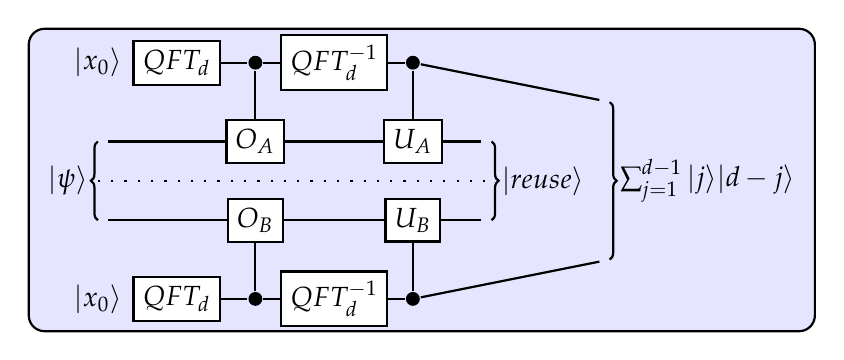
\begin{tikzpicture}[thick]
        %
        % `operator' will only be used by Hadamard (H) gates here.
        % `phase' is used for controlled phase gates (dots).
        % `surround' is used for the background box.
        \tikzstyle{operator} = [draw,fill=white,minimum size=1.5em] 
        \tikzstyle{phase} = [fill,shape=circle,minimum size=5pt,inner sep=0pt]
        \tikzstyle{surround} = [fill=blue!10,thick,draw=black,rounded corners=2mm]
        %
        % Bracket
        \draw[decorate,decoration={brace,mirror},thick] (0,-1) to
    	node[midway,left] (bracket1) {$\ket{\psi}$}
    	(0,-2);
        % Qubits
        \node at (0,0) (q1) {$\ket{x_0}$};
        \node at (0,-1) (q2) {};
        \node at (0,-2) (q3) {};
        \node at (0,-3) (q4) {$\ket{x_0}$};
        %
        % Column 1
        \node[operator] (op11) at (1,0) {$QFT_d$} edge [-] (q1);
        \node[operator] (op14) at (1,-3) {$QFT_d$} edge [-] (q4);
        %
        % Column 3
        \node[phase] (phase11) at (2,0) {} edge [-] (op11);
	\node[operator] (op22) at (2,-1) {$O_A$} edge [-] (q2);
	\node[operator] (op23) at (2, -2) {$O_B$} edge[-] (q3);
        \node[phase] (phase14) at (2,-3) {} edge [-] (op14);
        \draw[-] (phase11) -- (op22);
        \draw[-] (phase14) -- (op23);
        %
        % Column 4
        \node[operator] (op31) at (3,0) {$QFT_d^{-1}$} edge [-] (phase11);
        \node[operator] (op34) at (3,-3) {$QFT_d^{-1}$} edge [-] (phase14);
        %
        % Column 5
        \node[phase] (phase21) at (4,0) {} edge [-] (op31);
	\node[operator] (op42) at (4,-1) {$U_A$} edge [-] (op22);
	\node[operator] (op43) at (4, -2) {$U_B$} edge[-] (op23);
        \node[phase] (phase24) at (4,-3) {} edge [-] (op34);
        \draw[-] (phase21) -- (op42);
        \draw[-] (phase24) -- (op43);
        %
        % Column 6
        \node (end2) at (5,-1) {} edge [-] (op42);
        \node (end3) at (5,-2) {} edge [-] (op43);
        %
        % Bracket
        \draw[decorate,decoration={brace},thick] (5,-1) to
    	node[midway,right] (bracket) {$\ket{reuse}$}
    	(5,-2);
        %
        % Column 7
        \node (end1) at (6.5,-0.5) {} edge [-] (phase21);
        \node (end4) at (6.5,-2.5) {} edge [-] (phase24);
        % Dashed line
        \draw[loosely dotted] (0,-1.5) -- (5,-1.5);
        % Bracket
        \draw[decorate,decoration={brace},thick,] (6.5,-0.5) to
    	node[midway,right] (bracket2) {$\sum_{j=1}^{d-1}\ket{j}\ket{d-j}$}
    	(6.5,-2.5);
        %
        % Background Box
        \begin{pgfonlayer}{background} 
        \node[surround] (background) [fit = (q1) (op14) (bracket1)(bracket2)] {};
        \end{pgfonlayer}
        %
        \end{tikzpicture}
	\caption{The isometries $\Phi_{A,1} \x \Phi_{B,1}$.}
\end{figure}

The first isometry has the following steps:
\begin{enumerate}
	\item Append control register $\ket{x_0}_{A'}$ on Alice's side and $\ket{x_0}_{B'}$ on Bob's side;
	\item Apply Quantum Fourier Transform ($QFT_d$) to Alice and Bob's control registers;
	\item Apply Controlled-$O_{A/B}$ operations (i.e. if the control register is in state $\ket{x_k}_{A'/ B'}$, apply
	$O_{A/B}^k$.);
	\item Apply inverse Quantum Fourier Transform ($QFT_d^{-1}$) to the control registers;
	\item Apply Controlled-$U_{A/B}$ operations (i.e. If Alice's control register is in state $\ket{x_j}$, she applies
	$U_A^{\log_r (d-j)}$. If Bob's control register is in state $\ket{x_j}$, he applies $(U_B\ct)^{\log_r j}$).
\end{enumerate}

\begin{figure}[H]
\center
        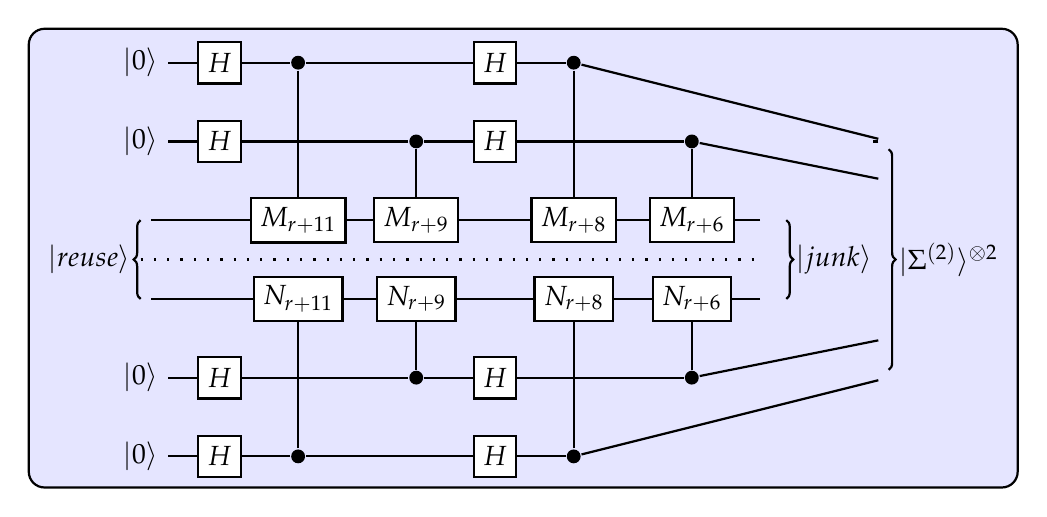
\begin{tikzpicture}[thick]
        %
        % `operator' will only be used by Hadamard (H) gates here.
        % `phase' is used for controlled phase gates (dots).
        % `surround' is used for the background box.
        \tikzstyle{operator} = [draw,fill=white,minimum size=1.5em] 
        \tikzstyle{phase} = [fill,shape=circle,minimum size=5pt,inner sep=0pt]
        \tikzstyle{surround} = [fill=blue!10,thick,draw=black,rounded corners=2mm]
        %
        % Bracket
        \draw[decorate,decoration={brace,mirror},thick] (0,-2) to
    	node[midway,left] (bracket1) {$\ket{reuse}$}
    	(0,-3);
        % Qubits
        \node at (0,0) (q1) {$\ket{0}$};
        \node at (0,-1) (q2) {$\ket{0}$};
        \node at (0,-2) (q3) {};
        \node at (0,-3) (q4) {};
        \node at (0,-4) (q5) {$\ket{0}$};
        \node at (0,-5) (q6) {$\ket{0}$};
        %
        % Column 1
        \node[operator] (op11) at (1,0) {$H$} edge [-] (q1);
        \node[operator] (op12) at (1,-1) {$H$} edge [-] (q2);
         \node[operator] (op15) at (1,-4) {$H$} edge [-] (q5);
        \node[operator] (op16) at (1,-5) {$H$} edge [-] (q6);
        %
        % Column 3
        \node[phase] (phase11) at (2,0) {} edge [-] (op11);
	\node[operator] (op23) at (2,-2) {$M_{r+11}$} edge [-] (q3);
	\node[operator] (op24) at (2, -3) {$N_{r+11}$} edge[-] (q4);
        \node[phase] (phase16) at (2,-5) {} edge [-] (op16);
        \draw[-] (phase11) -- (op23);
        \draw[-] (phase16) -- (op24);
        %
        % Column 4
        \node[phase] (phase12) at (3.5,-1) {} edge [-] (op12);
	\node[operator] (op33) at (3.5,-2) {$M_{r+9}$} edge [-] (op23);
	\node[operator] (op34) at (3.5, -3) {$N_{r+9}$} edge[-] (op24);
        \node[phase] (phase15) at (3.5,-4) {} edge [-] (op15);
        \draw[-] (phase12) -- (op33);
        \draw[-] (phase15) -- (op34);
        %
         % Column 5
        \node[operator] (op41) at (4.5,0) {$H$} edge [-] (phase11);
        \node[operator] (op42) at (4.5,-1) {$H$} edge [-] (phase12);
         \node[operator] (op45) at (4.5,-4) {$H$} edge [-] (phase15);
        \node[operator] (op46) at (4.5,-5) {$H$} edge [-] (phase16);
        %
        % Column 6
        \node[phase] (phase51) at (5.5,0) {} edge [-] (op41);
	\node[operator] (op53) at (5.5,-2) {$M_{r+8}$} edge [-] (op33);
	\node[operator] (op54) at (5.5, -3) {$N_{r+8}$} edge[-] (op34);
        \node[phase] (phase56) at (5.5,-5) {} edge [-] (op46);
        \draw[-] (phase51) -- (op53);
        \draw[-] (phase56) -- (op54);
        %
        % Column 7
        \node[phase] (phase62) at (7,-1) {} edge [-] (op42);
	\node[operator] (op63) at (7,-2) {$M_{r+6}$} edge [-] (op53);
	\node[operator] (op64) at (7, -3) {$N_{r+6}$} edge[-] (op54);
        \node[phase] (phase65) at (7,-4) {} edge [-] (op45);
        \draw[-] (phase62) -- (op63);
        \draw[-] (phase65) -- (op64);
        %
        % Bracket
        \node(end3) at (8, -2) {} edge [-] (op63);
        \node(end4) at (8, -3) {} edge [-] (op64);
        \draw[decorate,decoration={brace},thick] (8.2,-2) to
    	node[midway,right] (bracket) {$\ket{junk}$}
    	(8.2,-3);
        %
        % Column 7
        \node (end1) at (9.5,-1) {} edge [-] (phase51);
        \node(end2) at (9.5, -1.5) {} edge [-] (phase62);
       \node(end5) at (9.5, -3.5) {} edge [-] (phase65);
        \node (end6) at (9.5,-4) {} edge [-] (phase56);
        % Dashed line
        \draw[loosely dotted] (0,-2.5) -- (7.8,-2.5);
        \draw[solid] (end1) -- (9.3, -1);
        % Bracket
        \draw[decorate,decoration={brace},thick,] (9.5,-1.1) to
    	node[midway,right] (bracket2) {$\ket{\EPR{2}}^{\x 2}$}
    	(9.5,-3.9);
        %
        % Background Box
        \begin{pgfonlayer}{background} 
        \node[surround] (background) [fit = (q1) (op16) (bracket1)(bracket2)] {};
        \end{pgfonlayer}
        %
        \end{tikzpicture}
	\caption{The isometries $\Phi_{A,2} \x \Phi_{B,2}$.}
\end{figure}

The second isometry is the standard isometry used in the self-testing result of the Magic Square game \cite{wu2016}.
The only thing to note is that the state $\ket{reuse}$, which is on the same Hilbert space as $\ket{\psi}$ and produced by $\Phi_{A,1} \x \Phi_{B,1}$, is the input state to $\Phi_{A,2} \x \Phi_{B,2}$. In this sense, our isometry is a $2$-step sequential procedure.

%We first list the key relations needed for $\Phi_{A,1} \x \Phi_{B,1}$ to work.
%\begin{align}
%	&\ket{\psi} \appd{O(d^{5/4} r^{d/2} r^{1/4} \ep^{1/8})}\ket{\psi'} = \sum_{j=1}^{d-1} (U_A\ct U_B\ct)^{\log_r j} \ket{\psi_1},\\
%	&O_A(U_A\ct)^{\log_r j} \ket{\psi_1} \appd{O(\sd r^j \sr \qe)}\omega_d^{-r^j}  (U_A\ct)^j \ket{\psi_1}\\
%	&O_B(U_A\ct)^{\log_r j} \ket{\psi_1} \appd{O(\sd r^j \sr \qe)}\omega_d^{r^j}  (U_A\ct)^j \ket{\psi_1}.
%\end{align}
%The second isometry just requires properties of the Magic Square game, especially, the commutation relations in \cref{prop:lct_comm}.


\begin{proof}[Proof of \cref{thm:self-test}]
The proof takes two steps. 
We first show that 
\begin{align}
	\Phi_{A,1}\x\Phi_{B,1}(\ket{\psi}) \appd{O(d^{5/2} r^{d+1/2} \ep^{1/8})} \sqrt{d-1}\ket{\psi_1} \x \frac{1}{\sqrt{d-1}}\sum_{j=1}^{d-1} \ket{x_{d-j}}_{A'}\ket{x_j}_{B'}.
\end{align}
Then we show that there exists a state $\ket{junk}$ such that  
\begin{align}
\label{eq:phi2_result}
\Phi_{A,2} \x \Phi_{B,2} (\sqrt{d-1}\ket{\psi_1}) \appd{O(r\se)} \ket{junk} \x \ket{\EPR{2}}^{\x 2}.
\end{align}
Combining the two equations above we get that 
\begin{align*}
	&\quad\Phi_{A,2} \x \Phi_{B,2}( \Phi_{A,1} \x \Phi_{B,1} (\ket{\psi})) \\
	&\appd{O(d^{5/2} \sr \ep^{1/8})} \Phi_{A,2} \x \Phi_{B,2}(\sqrt{d-1} \ket{\psi_1}) \x\frac{1}{\sqrt{d-1}}\sum_{j=1}^{d-1} \ket{x_{d-j}}_{A'}\ket{x_j}_{B'} \\
	&\appd{O(r\se)} \ket{junk} \x \ket{\EPR{2}}^{\x 2} \x\frac{1}{\sqrt{d-1}}\sum_{j=1}^{d-1} \ket{x_{d-j}}_{A'}\ket{x_j}_{B'},
\end{align*}
where we use the fact that $\Phi_{A,2}\x \Phi_{B,2}$ only acts on the state $\ket{\psi_1}$.

\Cref{lm:decomp_psi} implies that $ \Phi_{A,1} \x \Phi_{B,1} (\ket{\psi}) \appd{O(d^{5/4} r^{d/2 +1/4} \ep^{1/8})}  \Phi_{A,1} \x \Phi_{B,1} (\ket{\psi'})$,  
so we focus on how the isometry evolves $\ket{\psi'}$.
The evolution is summarized below.
	\begin{align*}
		& \sum_{j=1}^{d-1} (U_A\ct U_B\ct)^{\log_r j} \ket{\psi_1} \ket{x_0}_{A'}\ket{x_0}_{B'}\\
		\xrightarrow[]{QFT_d}& \frac{1}{d}\sum_{k_1,k_2 = 0}^{d-1} \sum_{j=1}^{d-1} (U_A\ct U_B\ct)^{\log_r j}  \ket{\psi_1}\ket{x_{k_1}}_{A'}\ket{x_{k_2}}_{B'}\\
		\xrightarrow[]{\text{Controlled-}O_{A/B}}& \frac{1}{d}\sum_{k_1,k_2 = 0}^{d-1} \sum_{j=1}^{d-1} O_A^{k_1}(U_A\ct)^{\log_r j} O_B^{k_2}(U_B\ct)^{\log_r j}
		\ket{\psi_1} \ket{x_{k_1}}_{A'}\ket{x_{k_2}}_{B'}\\
		\appd{O(d^{5/2} r^{d} \sr \qe)}&\frac{1}{d} \sum_{k_1,k_2 = 0}^{d-1} \sum_{j=1}^{d-1} (U_A\ct U_B\ct)^{\log_r j}\omega_d^{(k_2-k_1)j}\ket{\psi_1} \ket{x_{k_1}}_{A'}\ket{x_{k_2}}_{B'}\\
		\xrightarrow[]{QFT_d^{-1}} &\frac{1}{d^2}\sum_{l_1,l_2 = 0}^{d-1}\sum_{k_1,k_2 = 0}^{d-1}\sum_{j=1}^{d-1} (U_A\ct U_B\ct)^{\log_r j} 
		\omega_d^{k_1(d-j-l_1)}\omega_d^{k_2(j-l_2)}\ket{\psi_1} \ket{x_{l_1}}_{A'}\ket{x_{l_2}}_{B'}\\
		= &\sum_{j=1}^{d-1}(U_A\ct U_B\ct)^{\log_r j} \ket{\psi_1} \ket{x_{d-j}}_{A'}\ket{x_j}_{B'} \\
		\xrightarrow[]{\text{Controlled-}U_{A/B}}& \sum_{j=1}^{d-1} U_A^{\log_r j} (U_A\ct)^{\log_r j} U_B^{\log_r j} (U_B\ct)^{\log_r j} \ket{\psi_1} \ket{x_{d-j}}_{A'}\ket{x_j}_{B'}\\
		=&\ket{\psi_1} \x \sum_{j=1}^{d-1} \ket{x_{d-j}}_{A'}\ket{x_j}_{B'}.
	\end{align*}
When we analyze the effect of the controlled-$O_{A/B}$, we applied \cref{eq:omega} repeatedly.
In summary, we have shown that
\begin{align}
	\Phi_{A,1}\x\Phi_{B,1}(\ket{\psi}) \appd{O(d^{5/2} r^{d+1/2} \ep^{1/8})} \sqrt{d-1} \ket{\psi_1} \x \frac{1}{\sqrt{d-1}}\sum_{j=1}^{d-1} \ket{x_{d-j}}_{A'}\ket{x_j}_{B'},
\end{align}
where we use the fact that $O(d^{5/2} r^{d+1/2} \ep^{1/8})$ dominates both $O(d^{5/4} r^{d/2+1/4} \ep^{1/8})$ and 
$O(d^{5/2} r^{d+1/2} \qe)$.
Since $\norm{\ket{\psi_1}}^2 \appd{O(r \se)} 1/(d-1)$, we know $ \sqrt{d-1} \norm{\ket{\psi_1}} \appd{O(\sd \sr\qe)} 1$.

To prove \cref{eq:phi2_result}, we first
recall that 
$\ket{\psi_1} 
	=\frac{1}{2} (M_{\nr+1}^0 + iM_{\nr+2}M_{\nr+1}^1 - iM_{\nr+2}M_{\nr+1}^0 + M_{\nr+1}^1) \ket{\psi}.
$
The other observation that we need is that 
\begin{align*}
	&\Phi_{A,2} \x \Phi_{B,2} (\ket{\psi_1})  \\
	= &\frac{1}{16} \sum_{\ua \ub \in\{0,1\}^4}
	M_{r+6}^{\ua(4)}N_{r+6}^{\ub(4)}M_{r+8}^{\ua(3)}N_{r+8}^{\ub(3)}M_{r+9}^{\ua(2)}N_{r+9}^{\ub(2)}M_{r+11}^{\ua(1)}N_{r+11}^{\ub(1)}
	\ket{\psi_1} \ket{\ua}_{A''} \ket{\ub}_{B''}
\end{align*}
For simplicity we define $M^{\ua} := M_{r+6}^{\ua(4)}M_{r+8}^{\ua(3)}M_{r+9}^{\ua(2)}M_{r+11}^{\ua(1)}$ and
$N^{\ub} := N_{r+6}^{\ub(4)}N_{r+8}^{\ub(3)}N_{r+9}^{\ub(2)}N_{r+11}^{\ub(1)} $.
We would like to show that 
\begin{align}
\label{eq:mua_comm}
M^{\ua} \ket{\psi_1} \appd{O(r\se)} \frac{1}{2} (M_{\nr+1}^0 + iM_{\nr+2}M_{\nr+1}^1 - iM_{\nr+2}M_{\nr+1}^0 + M_{\nr+1}^1)
M^{\ua} \ket{\psi},
\end{align}
for all $\ua \in \{0,1\}^4$,
%which implies that 
%\begin{align*}
%	\Phi_{A,2} \x &\Phi_{B,2} (\ket{\psi_1}) \appd{O(r\se)} \\
%	&\frac{1}{2} (M_{\nr+1}^0 + iM_{\nr+2}M_{\nr+1}^1 - iM_{\nr+2}M_{\nr+1}^0 + M_{\nr+1}^1)(\Phi_{A,2} \x \Phi_{B,2}(\ket{\psi}))
%\end{align*}
%because $N^{\ub}$ commutes with $\frac{1}{2} (M_{\nr+1}^0 + iM_{\nr+2}M_{\nr+1}^1 - iM_{\nr+2}M_{\nr+1}^0 + M_{\nr+1}^1)$
%for all $\ub \in \{0,1\}^4$.
which can be justified by \cref{prop:rel_comm}.
We show how to apply \cref{prop:rel_comm} to commute $M_{r+11}^{\ua(1)}$ through 
$\frac{1}{2} (M_{\nr+1}^0 + iM_{\nr+2}M_{\nr+1}^1 - iM_{\nr+2}M_{\nr+1}^0 + M_{\nr+1}^1)$ and then similar process can be repeated for $M_{r+9}, M_{r+8}$ and $M_{r+6}$,
\begin{align*}
	&\quad M_{r+11}^{\ua(1)} \frac{1}{2} (M_{\nr+1}^0 + iM_{\nr+2}M_{\nr+1}^1 - iM_{\nr+2}M_{\nr+1}^0 + M_{\nr+1}^1) \ket{\psi} \\
	&\appd{O(r\se)} \frac{1}{2}[ (M_{\nr+1}^0+M_{\nr+1}^1) M_{r+11}^{\ua(1)} -i M_{r+11}^{\ua(1)} M_{\nr+2}N_{\nr+1}] \ket{\psi} \\
	&\appd{O(r\se)} \frac{1}{2} [(M_{\nr+1}^0+M_{\nr+1}^1) M_{r+11}^{\ua(1)} - iM_{\nr+2}M_{r+11}^{\ua(1)} N_{\nr+1}] \ket{\psi} \\
	&\appd{O(r\se)}\frac{1}{2} [(M_{\nr+1}^0+M_{\nr+1}^1) M_{r+11}^{\ua(1)} - iM_{\nr+2}M_{r+11}^{\ua(1)} M_{\nr+1}] \ket{\psi} \\
	&\appd{O(r\se)}\frac{1}{2} [(M_{\nr+1}^0+M_{\nr+1}^1) M_{r+11}^{\ua(1)} - iM_{\nr+2}M_{\nr+1}M_{r+11}^{\ua(1)} ] \ket{\psi}.
\end{align*}
In summary, we have 
\begin{align}
	M^{\ua} N^{\ub} \ket{\psi_1} \appd{O(r\se)} \frac{1}{2} (M_{\nr+1}^0 + iM_{\nr+2}M_{\nr+1}^1 - iM_{\nr+2}M_{\nr+1}^0 + M_{\nr+1}^1)M^{\ua}N^{\ub} \ket{\psi}
\end{align}
for all $\ua, \ub \in \{0,1\}^4$, which implies that 
\begin{align*}
	\Phi_{A,2} \x& \Phi_{B,2}(\ket{\psi_1}) \appd{O(r\se)}\\
	 &\frac{1}{2} (M_{\nr+1}^0 + iM_{\nr+2}M_{\nr+1}^1 - iM_{\nr+2}M_{\nr+1}^0 + M_{\nr+1}^1)(\Phi_{A,2}\x\Phi_{B,2} (\ket{\psi}).
\end{align*}
At this point we can apply Lemma C.$1$ of \cite{wu2016} to $\Phi_{A,2}\x\Phi_{B,2} (\ket{\psi})$ and conclude that 
\begin{align}
	\Phi_{A,2} \x \Phi_{B,2}(\sqrt{d-1} \ket{\psi_1}) \appd{O(\sd r \se)} \ket{junk} \x \ket{\EPR{2}}^{\x 2},
\end{align} 
for some state $\ket{junk}$ whose norm can be deduced from the norm of $\ket{\psi_1}$.

In the rest of the proof, we only show how $\Phi_{A,1} \x \Phi_{B,1}$ acts on $O_A\ket{\psi}$ and $U_A\ket{\psi}$.

If the initial state is $O_A\ket{\psi}$, we first use the fact that 
$ \Phi_{A,1} \x \Phi_{B,1} (O_A\ket{\psi}) \appd{O(d^{5/4} r^{d/2+1/4} \ep^{1/8})}  \Phi_{A,1} \x \Phi_{B,1} (O_A\ket{\psi'})$, 
and then we calculate $\Phi_{A,1} \x \Phi_{B,1} (O_A\ket{\psi'})$ as
\begin{align*}
	O_A \ket{\psi'} \ket{x_0}_{A'}\ket{x_0}_{B'} =&  
		\sum_{j=1}^{d-1} O_A(U_A\ct U_B\ct)^{\log_r j}\ket{\psi_1}\ket{x_0}_{A'}\ket{x_0}_{B'}\\
		\appd{O(\sd r^{d+1/2} \ep^{1/4})}&\sum_{j=1}^{d-1}(U_A\ct U_B\ct)^{\log_r j} \omega_d^{-j} \ket{\psi_1} \ket{x_0}_{A'}\ket{x_0}_{B'}\\
		\xrightarrow[]{QFT_d} &\frac{1}{d}\sum_{j=1}^{d-1} \sum_{k_1,k_2 = 0}^{d-1}(U_A\ct U_B\ct)^{\log_r j} \omega_d^{-j} 
		\ket{\psi_1}\ket{x_{k_1}}_{A'}\ket{x_{k_2}}_{B'}\\
		\xrightarrow[]{\text{Controlled-}O_{A/B}}&\frac{1}{d}\sum_{j=1}^{d-1}\sum_{k_1,k_2 = 0}^{d-1} 
		 O_A^{k_1}(U_A\ct)^{\log_r j} O_B^{k_2}(U_B\ct)^{\log_r j} \omega_d^{-j} \ket{\psi_1} 
		 \ket{x_{k_1}}_{A'}\ket{x_{k_2}}_{B'}\\
		\appd{O(d^{5/2} r^{d+1/2}  \ep^{1/4})}& \frac{1}{d}\sum_{k_1,k_2 = 0}^{d-1} \sum_{j=1}^{d-1} (U_A\ct U_B\ct)^{\log_r j}
		\omega_d^{-j}\omega_d^{(k_2-k_1)j}\ket{\psi_1}
		 \ket{x_{k_1}}_{A'}\ket{x_{k_2}}_{B'}\\
		\xrightarrow[]{QFT_d^{-1}}& \sum_{j=1}^{d-1}  (U_A\ct U_B\ct)^{\log_r j}  
		\omega_d^{d-j}\ket{\psi_1} \ket{x_{d-j}}_{A'}\ket{x_j}_{B'}\\
		\xrightarrow[]{\text{Controlled-}U_{A/B}}&   \sqrt{d-1} \ket{\psi_1} \x  
		\frac{1}{\sqrt{d-1}}\sum_{j=1}^{d-1} \omega_d^{d-j}\ket{x_{d-j}}_{A'}\ket{x_j}_{B'}.
\end{align*}
The analysis for $\Phi_{A,1} \x\Phi_{B,1} (O_B \ket{\psi})$ is very similar.

If the initial state is $U_A\ket{\psi}$, we first use the fact that 
$ \Phi_{A,1} \x \Phi_{B,1} (U_A\ket{\psi}) \appd{O(d^{5/4}r^{d/2+1/4} \ep^{1/8})}  \Phi_{A,1} \x \Phi_{B,1} (U_A\ket{\psi'})$, 
and then we calculate $\Phi_{A,1} \x \Phi_{B,1} (U_A\ket{\psi'})$.
\begin{align*}
	U_A \ket{\psi'} \ket{x_0}_{A'}\ket{x_0}_{B'} =&  
		\sum_{j=1}^{d-1} U_A(U_A\ct U_B\ct)^{\log_r j}\ket{\psi_1} \ket{x_0}_{A'}\ket{x_0}_{B'}\\
		=&\sum_{j=1}^{d-1}(U_A\ct)^{\log_r j-1}  (U_B\ct)^{\log_r j} \ket{\psi_1} \ket{x_0}_{A'}\ket{x_0}_{B'}\\
		\xrightarrow[]{QFT_d} &\frac{1}{d}\sum_{j=1}^{d-1} \sum_{k_1,k_2 = 0}^{d-1}(U_A\ct)^{\log_r j-1} (U_B\ct)^{\log_r j} \ket{\psi_1}  \ket{x_{k_1}}_{A'}\ket{x_{k_2}}_{B'}\\
		\xrightarrow[]{\text{Controlled-}O_{A/B}}&\frac{1}{d}\sum_{j=1}^{d-1}\sum_{k_1,k_2 = 0}^{d-1} 
		 O_A^{k_1}(U_A\ct)^{\log_r j-1} O_B^{k_2}(U_B\ct)^{\log_r j} \ket{\psi_1} 
		 \ket{x_{k_1}}_{A'}\ket{x_{k_2}}_{B'}\\
		\appd{O(d^{5/2} r^{d+1/2} \qe)}& \frac{1}{d}\sum_{k_1,k_2 = 0}^{d-1} \sum_{j=1}^{d-1} (U_A\ct)^{\log_r j-1} (U_B\ct)^{\log_r j}
		\omega_d^{k_2j-k_1jr^{-1}}\ket{\psi_1}
		 \ket{x_{k_1}}_{A'}\ket{x_{k_2}}_{B'}\\
		\xrightarrow[]{QFT_d^{-1}}& \sum_{j=1}^{d-1}  (U_A\ct)^{\log_r j-1} (U_B\ct)^{\log_r j}  
		\ket{\psi_1} \ket{x_{(d-j)r^{-1}}}_{A'}\ket{x_j}_{B'}\\
		\xrightarrow[]{\text{Controlled-}U_{A/B}}& \sqrt{d-1} \ket{\psi_1} \x  
		\frac{1}{\sqrt{d-1}} \sum_{j=1}^{d-1} \ket{x_{(d-j)r^{-1}}}_{A'}\ket{x_j}_{B'},
\end{align*}
where we use the fact that $(d-j)r^{-1} \equiv d -jr^{-1} \pmod{d}$.
The analysis for $\Phi_{A,1} \x\Phi_{B,1} (U_B \ket{\psi})$ is very similar.
\end{proof}

%%-----------------------------------------------------------------
%\subsection{Self-test}
%%-----------------------------------------------------------------
%\hl{This subsection needs to be formalized.}
%We give a formal version of \cref{thm:pr_2} first and then prove it.
%\begin{theorem}
%\label{thm:selftest}
%	If a quantum strategy using the shared state $\ket{\psi}$ achieves the ideal 2-party correlation $C(\dr{r})$ where $d$ is an odd
%	prime number with primitive root $r \in \{2,3,5\}$, then there exist local isometries $\Phi_A$ and $\Phi_B$, and a state $\ket{junk}$ such 
%	that $\Phi_A\x\Phi_B \ket{\psi} = \ket{\EPR{d-1}} \x \ket{junk}$.
%\end{theorem}
%\begin{proof}
%Suppose Alice and Bob achieve the optimal correlation with the quantum strategy $(\ket{\psi}, \{A_x\}, \{B_y\})$
%for all $x,y \in \calX \times \calY$ .
%The observables $A_x$ and $B_y$ and the shared state $\ket{\psi}$ shall not be confused with the ones used in the optimal strategy.
%By Lemma~$4.3$ of Ref.~\cite{coladan2017}, we can extract an operator solution from the perfect winning strategy 
%of the linear system game $\LS_r$. 
%For each variable $\{ x_i \}_{i=1}^{n_r}$, Alice and Bob has operators $A_i$ and $B_i$ respectively.
%The condition that they agree with assignment to variables means that 
%\begin{align}
%	\bra{\psi} A_i \otimes \overline{B_i} \ket{\psi} = 1 \Rightarrow A_i \otimes \overline{B_i} \ket{\psi} = \ket{\psi}
%	\text{ for } 1 \leq i \leq n_r
%\end{align}
%and the condition that Alice's assignments satisfy the constraint means that 
%\begin{align}
%	\Tr(\rho_A \Pi_{j: H(i,j) \neq 0} A_j) = \Tr(\rho_A) \text{ for all } 1 \leq i \leq m_r
%\end{align}
%where $\rho_A =  \Tr_B(\ketbra{\psi}{\psi})$. 
%Similarly we define $\rho_B = \Tr_A(\ketbra{\psi}{\psi})$.
%For any $\ket{v} \in \supp(\rho_A)$,
%we have 
%\begin{align}
%\Pi_{j:H(i,j) \neq 0} A_j \ket{v} = \ket{v} \text{ for all } 1 \leq i \leq m_r.
%\end{align}
%Since the relation $uxu^{-1} = x^r$, where $r$ is the primitive root of $d$, is embedded in this linear system game, we know
%\begin{align}
%	A_3A_4 A_1A_2 (A_3A_4)^\dagger \ket{v}= (A_1A_2)^r \ket{v} \text{ for all } \ket{v} \in \supp(\rho_A).
%\end{align}
%For simplicity, we define $X_A = A_1A_2$ and $U_A=A_3A_4$ such that
%the condition is equivalent to
%\begin{align}
%	\label{eq:ux_relation}
%	U_AX_AU_A^\dagger \ket{v} = X_A^r \ket{v} \text{ for all } \ket{v} \in \supp(\rho_A).
%\end{align}
%We will come back to the implication of this condition later.
%
%Suppose $A_{m_r+1} = A_\ast^\diamond- A_\ast^\perp = \Pi_{V_A} - \Pi_{V_A^\perp}$m, where $V_A$ is a
%$2m$-dimensional vector space and $\Pi_{V_A}$ is the projector onto it. The reason why it has dimension $2m$
%will be clear shortly. On Bob's side, we also have $B_{n_r+1} = B_\ast^\diamond- B_\ast^\perp = \Pi_{V_B} - \Pi_{V_B^\perp}$.
%Recall that from the extended weighted CHSH test, we know
%\begin{align}
%	A_\ast^\diamond \ket{\psi} = B_\ast^\diamond \ket{\psi} = A_\ast^\diamond \x B_\ast^\diamond \ket{\psi},
%\end{align}
%which implies that with an appropriate change of basis, we can get $V_A = V_B$, so in the rest of the proof
%we drop the subscript of $V$.
%By \cref{lm:chsh_comp} and \cref{prop:2d-subspace}, we know $V$ consists of $\omega_d$-eigenvectors and $\omega_d^{-1}$ eigenvectors of 
%$X_A$, so we can write 
%\begin{align}
%	\Pi_{V} = \Pi_{V_1} + \Pi_{V_{d-1}},
%\end{align}
%where $\Pi_{V_{1}}$ is the projector onto the $\omega_d$-eigenspace of $X_A$ and $\Pi_{V_{d-1}}$ is the projector 
%onto the $\omega_d^{-1}$-eigenspace of $X_A$.
%\hl{Here what we need is that $\Pi_{V_1,A} \ket{\psi} = \Pi_{V_{d-1},B} \ket{\psi} = \Pi_{V_1,A}\Pi_{V_{d-1},B}\ket{\psi}$
%and $\Pi_{V_1,B} \ket{\psi} = \Pi_{V_{d-1},A} \ket{\psi} = \Pi_{V_1,B}\Pi_{V_{d-1},A}\ket{\psi}$.
%This is not proved because $\Pi_{V_1}$ and $\Pi_{V_{d-1}}$ are not in the strategy.}
%Suppose $\ket{x_{1}} \in V_{1}$, then $X_A \ket{x_{1}} = \omega_d \ket{x_{1}}$.
%By \cref{eq:ux_relation} we can calculate that
%\begin{align}
%\label{eq:ladder}
% X_AU_A^\dagger \ket{x_{1}} = U_A^\dagger X_A^r \ket{x_{1}} = \omega_d^r U_A^\dagger \ket{x_{1}},
%\end{align}
%so $U_A^\dagger \ket{x_{1}}$ is an eigenvector of $X_A$ with eigenvalue $\omega_d^r$.
%By induction, we know $X_A (U_A^\dagger)^i \ket{x_{1}} = \omega_d^{r^i} (U_A^\dagger)^i\ket{x_{1}}$. 
%From the set $\{(U_A^\dagger)^i \Pi_{V_1} (U_A)^i \}_{i=0}^{d-2}$, we can identify $\Pi_{V_i}$ for $i = 1 \dots  d-1$
%such that $\Pi_{V_i}$ is the projector onto the $\omega_d^i$-eigenspace of $X_A$,
%\hl{Actually, we are not sure about the containment between $\supp((U_A\ct)^{\log_r(d-1)} \Pi_{V_1} U_A^{\log_r(d-1)})$ and 
%$\supp(\Pi_{V_{d-1}})$, so we cannot say that $\Pi_{V_{d-1}} = (U_A\ct)^{\log_r(d-1)} \Pi_{V_1} U_A^{\log_r(d-1)}$.}
%and 
%\begin{align}
% \cup_{i \in [d-1]+1} V_i \subset \supp(\rho_A).
%\end{align}
%Since unitary transformation does not change the rank of a matrix, we know $\rank(\Pi_{V_1}) = \rank(\Pi_{V_{i}}) =N$
%for $ i =1 \dots d-1$.
%We pick a basis for $V_1$ such that 
%\begin{align}
%	\Pi_{V_1} =  \sum_{j=1}^m \ketbra{x_{1,j}}{x_{1,j}},
%\end{align}
%then we can construct 
%\begin{align}
% \Pi_{V_i} = \sum_{j=1}^m \ketbra{x_{i,j}}{x_{i,j}},
%\end{align}
%where $\ket{x_{i,j}} = (U\ct)^{k_i} \ket{x_{1,j}}$ for $r^{k_i} \equiv i \pmod{d}$ and $1 \leq j \leq m$.
%By \cref{eq:ux_relation} we also know that $U_A \ket{x_{i,j}} = \ket{x_{i/2,j}}$ for $i = 1,2 \dots d-1$.
%In order to apply \cref{lm:ux_independ}, we construct $m$ subspaces $\{W_j\}_{j=1}^m$ where 
%\begin{align}
%	W_j = \spn( \{ \ket{x_{i,j}} \}_{i=1}^{d-1} )
%\end{align}
%The subspace $W_j$ is orthogonal to $W_{j'}$ for $j \neq j'$, and
%$U_A$ and $X_A$ satisfy the condition of \cref{lm:ux_independ} when their actions are 
%restricted to each $W_j$.
%Similar argument also applies to operator $X_B$ and $U_B$ on Bob's side.


%With an appropriate change of basis, we 
%assume that $\ket{\psi} = \vc(\tau)$ for some $\tau \in L(\supp(\rho_A))$
%The consistency condition is equivalent to
%\begin{align}
%\label{eq:con_tau}
%	A_i \tau B_i^\dagger = \tau.
%\end{align}
%Substituting $i=1,2$ into \cref{eq:con_tau}, we get 
%\begin{align}
%	X_A \tau X_A^\dagger = A_1A_2\tau B_2^\dagger B_1^\dagger = A_1\tau B_1^\dagger = \tau.
%\end{align}
%Similar argument gives us that 
%\begin{align}
%	U_A \tau U_A^\dagger = \tau.
%\end{align}
%Then we can conclude that for any $k \in \{0,1 \dots d-2\}$ and $l \in \{1,2\dots d-1\}$
%\begin{align}
%	U_A^kX_A^l \tau (U_A^kX_A^l)^\dagger = \tau.
%\end{align}
%Let $\Pi_{W_j}$ be the projector onto $W_j$. 
%By \cref{lm:ux_independ}, $\Pi_{W_j} \tau \Pi_{W_j}$ commutes with all the $(d-1) \times (d-1)$ matrices, which means that 
%\begin{align}
%	\label{eq:d-1}
%	\Pi_{W_j} \tau \Pi_{W_j}  = c_j \1_{W_j} \text{ for } j = 1\dots m.
%\end{align}
%In the vector form, we know
%\begin{align}
%	\sum_{j =1}^N \Pi_{W_j} \ket{\psi} =\sum_{i=1}^{d-1} \sum_{j=1}^m c_j \ket{x_{i,j}}\ket{x_{i,j}}. 
%\end{align}
%Recalling the fact that 
%\begin{align}
%\norm{ \Pi_{V_1} + \Pi_{V_{d-1}} \ket{\psi}}^2 = \norm{\Pi_{V_1} \ket{\psi}}^2 + \norm{\Pi_{V_{d-1}} \ket{\psi}}^2 = \frac{2}{d-1},
% \end{align}
% it means that 
% \begin{align}
% 	2 \sum_{j=1}^m \norm{c_j}^2 = \frac{2}{d-1}.
% \end{align}
% Then we can calculate the norm of $\sum_{j =1}^m \Pi_{W_j} \ket{\psi}$, which is
% \begin{align}
% \norm{\sum_{j =1}^m \Pi_{W_j} \ket{\psi}}^2 = \sum_{i=1}^{d-1} \sum_{j=1}^m \norm{c_j}^2 = 1 = \norm{\ket{\psi}}^2.
% \end{align}
% We can conclude that $\supp{\rho_A} = \cup_{i=1}^{d-1} V_i$ and 
% \begin{align}
% 	\ket{\psi} = \sum_{i=1}^{d-1}\sum_{j=1}^m c_j \ket{x_{i,j}}\ket{x_{i,j}}.
% \end{align}
% 
%The last step is to construct the local isometries $\Phi_A$ and $\Phi_B$ that can produce $\ket{\EPR{d-1}}$ from $\ket{\psi}$.
%To help understanding, we draw a diagram to demonstrate the isometry first and then show
%how this isometry works.
%\begin{figure}[H]
%\center
%        \begin{tikzpicture}[thick]
%        %
%        % `operator' will only be used by Hadamard (H) gates here.
%        % `phase' is used for controlled phase gates (dots).
%        % `surround' is used for the background box.
%        \tikzstyle{operator} = [draw,fill=white,minimum size=1.5em] 
%        \tikzstyle{phase} = [fill,shape=circle,minimum size=5pt,inner sep=0pt]
%        \tikzstyle{surround} = [fill=blue!10,thick,draw=black,rounded corners=2mm]
%        %
%        % Bracket
%        \draw[decorate,decoration={brace,mirror},thick] (0,-1) to
%    	node[midway,left] (bracket1) {$\ket{\psi}$}
%    	(0,-2);
%        % Qubits
%        \node at (0,0) (q1) {$\ket{0}$};
%        \node at (0,-1) (q2) {};
%        \node at (0,-2) (q3) {};
%        \node at (0,-3) (q4) {$\ket{0}$};
%        %
%        % Column 1
%        \node[operator] (op11) at (1,0) {$QFT_d$} edge [-] (q1);
%        \node[operator] (op14) at (1,-3) {$QFT_d$} edge [-] (q4);
%        %
%        % Column 3
%        \node[phase] (phase11) at (2,0) {} edge [-] (op11);
%	\node[operator] (op22) at (2,-1) {$X_A$} edge [-] (q2);
%	\node[operator] (op23) at (2, -2) {$X_B$} edge[-] (q3);
%        \node[phase] (phase14) at (2,-3) {} edge [-] (op14);
%        \draw[-] (phase11) -- (op22);
%        \draw[-] (phase14) -- (op23);
%        %
%        % Column 4
%        \node[operator] (op31) at (3,0) {$QFT_d^{-1}$} edge [-] (phase11);
%        \node[operator] (op34) at (3,-3) {$QFT_d^{-1}$} edge [-] (phase14);
%        %
%        % Column 5
%        \node[phase] (phase21) at (4,0) {} edge [-] (op31);
%	\node[operator] (op42) at (4,-1) {$U_A$} edge [-] (op22);
%	\node[operator] (op43) at (4, -2) {$U_B$} edge[-] (op23);
%        \node[phase] (phase24) at (4,-3) {} edge [-] (op34);
%        \draw[-] (phase21) -- (op42);
%        \draw[-] (phase24) -- (op43);
%        %
%        % Column 6
%        \node (end2) at (5,-1) {} edge [-] (op42);
%        \node (end3) at (5,-2) {} edge [-] (op43);
%        %
%        % Bracket
%        \draw[decorate,decoration={brace},thick] (5,-1) to
%    	node[midway,right] (bracket) {$\ket{junk}$}
%    	(5,-2);
%        %
%        % Column 7
%        \node (end1) at (6.5,-0.5) {} edge [-] (phase21);
%        \node (end4) at (6.5,-2.5) {} edge [-] (phase24);
%        % Dashed line
%        \draw[loosely dotted] (0,-1.5) -- (5,-1.5);
%        % Bracket
%        \draw[decorate,decoration={brace},thick,] (6.5,-0.5) to
%    	node[midway,right] (bracket2) {$\ket{\EPR{d-1}}$}
%    	(6.5,-2.5);
%        %
%        % Background Box
%        \begin{pgfonlayer}{background} 
%        \node[surround] (background) [fit = (q1) (op14) (bracket1)(bracket2)] {};
%        \end{pgfonlayer}
%        %
%        \end{tikzpicture}
%	\caption{The isometries $\Phi_A$ and $\Phi_B$.}
%\end{figure}
%The isometry maps the state $\ket{\psi}$ in the following steps:
%\begin{enumerate}
%	\item Append $\ket{0}_A$ on Alice's side and $\ket{0}_B$ on Bob's side as control registers, and
%	the state becomes $\ket{\psi} \ket{0}_A \ket{0}_B$;
%	\item Apply $QFT_d$ to the control registers, and the state becomes
%	\begin{align}
%		\frac{1}{d} \sum_{k_1,k_2 =0}^{d-1} \ket{\psi} \ket{k_1}_A \ket{k_2}_B;
%	\end{align}
%	\item Apply $X_A^{k_1}$ to Alice's share of $\ket{\psi}$ and $X_B^{k_2}$ to Bob's share controlled
%	by the control registers, and the state becomes
%	\begin{align}
%		&\frac{1}{d} \sum_{k_1,k_2 =0}^{d-1}X_A^{k_1} X_B^{k_2}\ket{\psi} \ket{k_1}_A \ket{k_2}_B\\
%		=&\frac{1}{d} \sum_{k_1,k_2 =0}^{d-1} \sum_{i=1}^{d-1}\sum_{j=1}^m c_j X_A^{k_1}\ket{x_{i,j}}_A X_B^{k_2}\ket{x_{i,j}}_B
%		\ket{k_1}_A \ket{k_2}_B\\
%		=&\frac{1}{d} \sum_{k_1,k_2 =0}^{d-1} \sum_{i=1}^{d-1}\sum_{j=1}^m c_j \omega_d^{k_1i+k_2i} \ket{x_{i,j}}_A\ket{x_{i,j}}_B
%		\ket{k_1}_A \ket{k_2}_B;
%	\end{align}
%	\item Apply $QFT_d^{-1}$ to the control registers, and the state becomes
%	\begin{align}
%		&\frac{1}{d^2} \sum_{l_1,l_2 =0}^{d-1}\sum_{i=1}^{d-1}\sum_{j=1}^m c_j \omega_d^{k_1(i-l_1)+k_2(i-l_2)} \ket{x_{i,j}}_A\ket{x_{i,j}}_B
%		\ket{l_1}_A \ket{l_2}_B\\
%		=& \sum_{i=1}^{d-1}\sum_{j=1}^m c_j \ket{x_{i,j}}_A\ket{x_{i,j}}_B \ket{i}_A \ket{i}_B;
%	\end{align}
%	\item Let $n_i$ satisfy the condition $r^{n_i} \equiv i \pmod{d}$, apply $U_A^{(i)} = U_A^{n_i}$ to Alice's share of $\ket{\psi}$ and $U_B^{(i)} = U_B^{n_i}$ to Bob's share controlled
%	by the control registers, and the state becomes
%	\begin{align}
%		&\sum_{i=1}^{d-1}\sum_{j=1}^m c_j U_A^{(i)}\ket{x_{i,j}}_A U_B^{(i)}\ket{x_{i,j}}_B \ket{i}_A\ket{i}_B \\
%		=&\sum_{i=1}^{d-1} \sum_{j=1}^m c_j \ket{x_{i r^{-n_i} ,j}}_A \ket{x_{i r^{-n_i},j}}_B \ket{i}_A\ket{i}_B\\
%		=& \sum_{i=1}^{d-1} \sum_{j=1}^m c_j \ket{x_{i i^{-1},j}}_A \ket{x_{i i^{-1},j}}_B \ket{i}_A\ket{i}_B\\
%		= &\left(\sum_{j=1}^m c_j \ket{x_{1,j}}_A \ket{x_{1,j}}_B\right) \x \sum_{i=1}^{d-1} \ket{i}_A\ket{i}_B\\
%		=&\sqrt{d-1} \left(\sum_{j=1}^m c_j \ket{x_{1,j}}_A \ket{x_{1,j}}_B\right) \x 
%		\frac{1}{\sqrt{d-1}}\sum_{i=1}^{d-1}\ket{i}_A\ket{i}_B\\
%		=&\sqrt{d-1} \left(\sum_{j=1}^m c_j \ket{x_{1,j}}_A \ket{x_{1,j}}_B\right) \x \ket{\EPR{d-1}},
%	\end{align}
%	where in the last line we used the fact that $\norm{\sum_{j=1}^m c_j \ket{x_{1,j}}_A \ket{x_{1,j}}_B} = 1/\sqrt{d-1}$.
%\end{enumerate}
%
%If the initial state is $X_A\ket{\psi}$, the isometry maps the state as following
%\begin{align}
%	X_A\ket{\psi} \to &X_A\ket{\psi}\ket{0}_A\ket{0}_B\\
%	\to &\frac{1}{d} \sum_{k_1,k_2 =0}^{d-1} X_A\ket{\psi} \ket{k_1}_A \ket{k_2}_B \\
%	\to &\frac{1}{d} \sum_{k_1,k_2 =0}^{d-1} X_A^{k_1+1} X_B^{k_2}\ket{\psi} \ket{k_1}_A \ket{k_2}_B \\
%	=&\frac{1}{d} \sum_{k_1,k_2 =0}^{d-1} \sum_{i=1}^{d-1}\sum_{j=1}^m c_j \omega_d^i\omega_d^{(k_1+k_2)i} \ket{x_{i,j}}_A\ket{x_{i,j}}_B
%		\ket{k_1}_A \ket{k_2}_B\\
%	\to &\frac{1}{d^2}\sum_{k_1,k_2 =0}^{d-1} \sum_{i=1}^{d-1}\sum_{j=1}^m c_j \omega_d^i\omega_d^{(k_1-l_1)i+(k_2-l_2)i} \ket{x_{i,j}}_A\ket{x_{i,j}}_B
%		\ket{l_1}_A \ket{l_2}_B\\
%	=&\sum_{i=1}^{d-1}\sum_{j=1}^m c_j \omega_d^i \ket{x_{i,j}}_A\ket{x_{i,j}}_B \ket{i}_A \ket{i}_B\\
%	\to& \sum_{i=1}^{d-1}\sum_{j=1}^m c_j \omega_d^i U_A^{(i)}\ket{x_{i,j}}_A U_B^{(i)}\ket{x_{i,j}}_B \ket{i}_A\ket{i}_B\\
%	=&\sum_{i=1}^{d-1}\sum_{j=1}^m c_j \omega_d^i \ket{x_{1,j}}_A \ket{x_{1,j}}_B \ket{i}_A\ket{i}_B\\
%	=&\sqrt{d-1} \left(\sum_{j=1}^m c_j \ket{x_{1,j}}_A \ket{x_{1,j}}_B\right) \x 
%		\frac{1}{\sqrt{d-1}} \sum_{i=1}^{d-1}\omega_d^i \ket{i}_A\ket{i}_B\\
%	=& \sqrt{d-1} \left(\sum_{j=1}^m c_j \ket{x_{1,j}}_A \ket{x_{1,j}}_B\right) \x \tX_A \ket{\EPR{d-1}},
%\end{align}
%where $\tX_A$ is the ideal $X$ operator.
%The case of $X_B\ket{\psi}$ is similar, so we omit it here. 
%
%If the initial state is $U_A\ket{\psi}$, the isometry maps the state as following
%\begin{align}
%	U_A\ket{\psi} \to &U_A\ket{\psi}\ket{0}_A\ket{0}_B\\
%	\to &\frac{1}{d} \sum_{k_1,k_2 =0}^{d-1} U_A\ket{\psi} \ket{k_1}_A \ket{k_2}_B \\
%	= &\frac{1}{d} \sum_{k_1,k_2=0}^{d-1} \sum_{i=1}^{d-1}\sum_{j=1}^m c_j U_A\ket{x_{i,j}}_A\ket{x_{i,j}}_B
%		\ket{k_1}_A \ket{k_2}_B\\
%	= & \frac{1}{d} \sum_{k_1,k_2=0}^{d-1} \sum_{i=1}^{d-1}\sum_{j=1}^m c_j \ket{x_{i r^{-1} ,j}}_A\ket{x_{i,j}}_B
%		\ket{k_1}_A \ket{k_2}_B\\
%	\to &\frac{1}{d} \sum_{k_1,k_2 =0}^{d-1} \sum_{i=1}^{d-1}\sum_{j=1}^m c_j X_A^{k_1} \ket{x_{i r^{-1} ,j}}_A
%	X_B^{k_2}\ket{x_{i,j}}_B  \ket{k_1}_A \ket{k_2}_B \\
%	=&\frac{1}{d} \sum_{k_1,k_2 =0}^{d-1} \sum_{i=1}^{d-1}\sum_{j=1}^m c_j \omega_d^{k_1 i/r}\omega_d^{k_2i} \ket{x_{ir^{-1},j}}_A\ket{x_{i,j}}_B
%		\ket{k_1}_A \ket{k_2}_B\\
%	\to &\frac{1}{d^2}\sum_{k_1,k_2 =0}^{d-1} \sum_{i=1}^{d-1}\sum_{j=1}^m c_j \omega_d^{k_1(i/r-l_1)}\omega_d^{(k_2(i-l_2)} \ket{x_{ir^{-1},j}}_A\ket{x_{i,j}}_B
%		\ket{l_1}_A \ket{l_2}_B\\
%	=&\sum_{i=1}^{d-1}\sum_{j=1}^m c_j  \ket{x_{ir^{-1},j}}_A\ket{x_{i,j}}_B \ket{ir^{-1}}_A \ket{i}_B\\
%	\to& \sum_{i=1}^{d-1}\sum_{j=1}^m c_j U_A^{(ir^{-1})}\ket{x_{ir^{-1},j}}_A U_B^{(i)}\ket{x_{i,j}}_B \ket{i}_A\ket{i}_B\\
%	=&\sum_{i=1}^{d-1}\sum_{j=1}^m c_j \ket{x_{1,j}}_A \ket{x_{1,j}}_B \ket{ir^{-1}}_A\ket{i}_B\\
%	=&\sqrt{d-1} \left(\sum_{j=1}^m c_j \ket{x_{1,j}}_A \ket{x_{1,j}}_B\right) \x 
%		\frac{1}{\sqrt{d-1}} \sum_{i=1}^{d-1}\ket{ir^{-1}}_A\ket{i}_B\\
%	=& \sqrt{d-1} \left(\sum_{j=1}^m c_j \ket{x_{1,j}}_A \ket{x_{1,j}}_B\right) \x \tU_A \ket{\EPR{d-1}},
%\end{align}
%where $\tU_A$ is the ideal $U$ operator on Alice's side.
%The derivation is similar when $U_B$ is applied, so we omit it here.
%\end{proof}
%The effect of $\CHSH_X$ and $\SVT_X$ is that we have a set $\{ \ket{x_i} \}_{i \in [d]} \in \supp(\rho_A)$ such that
%\begin{align}
%	X \ket{x_i} = \omega_d^i \ket{x_i}.
%\end{align}
%The other effect of $\SVT_X$ is that we know 
%\begin{align}
%	\tA_\triangle^\diamond \rho_A \tA_\triangle^\diamond = \frac{1}{d} \ketbra{x_0}{x_0} = \frac{1}{d} \tA_\triangle^\diamond.
%\end{align}
%\hl{\textbf{Question}: Can we show $\Tr(\ketbra{x_2}{x_2} \rho_A) = 1/d$?}

%We remark that our proof works for any odd prime number with primitive root $r$.
%However, since there is no upper-bound of $r$ for a general prime number $d$, we 
%cannot claim the corresponding correlation $C(d)$ is constant-sized. On the other
%hand, since $r$ is usually much smaller than $d$, our result implies a more efficient
%way to test EPR pairs of prime local dimension than the one proposed in Ref.~\cite{cgs2017}.
%The size of our correlation grows linearly in $r$ whereas the Coladangelo \textit{et. al.}'s
%method uses correlation grows linearly in $d$.

\bibliographystyle{alphaurl}
\bibliography{quantum_correlation}
\appendix
%========================================
\section{The proof of \cref{thm:selftest} }
\label{sec:selftest}
%========================================
This proof follows the same line of argument in Appendix A of Ref.~\cite{bamps2015}.
We first find two sum-of-square decompositions of $2\sqrt{\alpha^2+1} \1 - \I_\alpha$,
where $\I_\alpha$ is expressed in terms of $\{M_x\}$ and $\{N_y\}$.
The decompositions allow us to determine some key relations between Alice and Bob's observables
and their shared state, which will be used to draw the conclusion.

\begin{proof}
The first step is to find a sum-of-square decomposition of 
the following Bell expression
\begin{align}
	\bar{\I}_\alpha = 2\sqrt{\alpha^2+1} \1 - \I_\alpha
	= \frac{2}{\sin(\mu)} \1 - \frac{\cos(\mu)}{\sin(\mu)}(M_1N_1+M_1N_2) -  M_2N_1 + M_2N_2.
\end{align} 
With the notation $c:= \cos(\mu)$, $s := \sin(\mu)$ and 
\begin{align*}
	&Z_A = M_1 && X_A = M_2\\
	&Z_B = \frac{N_1+N_2}{2c} && X_B = \frac{N_1-N_2}{2s},
\end{align*}
the two SOS decompositions that we use are
\begin{align}
	\label{eq:sos1}&\bar{\I}_\alpha = \frac{s \bar{\I}_\alpha^2 + 4sc^2(Z_AX_B+X_AZ_B)^2}{4},\\
	\label{eq:sos2}&\bar{\I}_\alpha = \frac{c^2}{s}(Z_A-Z_B)^2 + s(X_A-X_B)^2.
\end{align}
The verification is omitted here. From the SOS decomposition, we establish \cref{eq:za-zb,eq:xa-xb,eq:xazb,eq:zaxb,eq:zaxa,eq:zaxaxbzb}.
We define
\begin{align*}
	&S_1 = \frac{\sqrt{s}}{2} \bar{\I}_\alpha, &&
	S_2 = \sqrt{s}c(Z_AX_B+ X_AZ_B),\\
	&S_3 = \frac{c}{\sqrt{s}}(Z_A-Z_B), &&
	S_4 = \sqrt{s}(X_A-X_B)
\end{align*}
then 
\begin{align}
\bar{\I}_\alpha = S_1^2 + S_2^2 = S_3^2 + S_4^2
\end{align}
The fact that the quantum strategy $(\ket{\psi}, \{M_x\}_{x=1,2}, \{N_{y }\}_{y=1,2}$ achieves that 
$\ip{\bar{\I}_\alpha} \leq \epsilon$ implies that
$\bra{\psi} S_i^2 \ket{\psi} \leq \ep$, and equivalently, $\norm{S_i \ket{\psi}} \leq \se$ for $i = 1,2,3,4$.
From the definitions of $S_i$'s, we can get that 
\begin{align}
	&\norm{(X_AZ_B+X_BZ_A)\ket{\psi}} \leq \frac{1}{c\sqrt{s}} \se\\
	&\norm{(Z_A-Z_B)\ket{\psi}} \leq \frac{\sqrt{s}}{c} \se\\
	&\norm{(X_A-X_B)\ket{\psi}} \leq \frac{1}{\sqrt{s}} \se.
\end{align}
The first and the second inequality give us that 
\begin{align}
	\norm{ [Z_A(\1+X_B) - (\1-X_A)Z_B] \ket{\psi} } 
	\leq \norm{(X_AZ_B+X_BZ_A)\ket{\psi}} + \norm{(Z_A-Z_B)\ket{\psi}}
	\leq \frac{s+1}{c\sqrt{s}} \se.
\end{align}
Similarly, the first and the third inequality give us that 
\begin{align}
	\norm{[X_A(\1+Z_B) - X_B(\1-Z_A)] \ket{\psi}} \leq \frac{c+1}{c\sqrt{s}} \se.
\end{align}
Since $Z_AX_A +X_A Z_A = \frac{S_2}{c\sqrt{s}} + \frac{\sqrt{s}\tilde{X}_AS_3}{c} + \frac{\tilde{Z}_AS_4}{\sqrt{s}}$, we can deduce that
\begin{align}
	\norm{ (Z_A X_A+X_AZ_A)\ket{\psi}} \leq \frac{1+c+s}{c\sqrt{s}} \se.
\end{align}
To prove \cref{eq:zaxaxbzb}, we switch to the approximate relation form and derive that 
\begin{align}
	X_AZ_A \ket{\psi} &\appd{\frac{1+c+s}{c\sqrt{s}} \se}  -Z_AX_A \ket{\psi} \\
	&\appd{\frac{\sqrt{s}}{c} \se} -Z_AX_B \ket{\psi} \\
	&\appd{\frac{1}{s^{3/2} }\se} -X_BZ_B\ket{\psi},
\end{align}
where in the last line we use the fact $\norm{X_B} \leq 1/s$.

Now we introduce the isometries $\Phi_A$ and $\Phi_B$ mentioned in the statement of the theorem.
They are the same as the ones used in Ref.~\cite{bamps2015}.
To construct $\Phi_A$ and $\Phi_B$ we need to regularize $Z_B$ and $X_B$ to make sure the corresponding operations 
are unitary in the isometries. We define $Z_B^\ast$ to be the operator obtained from $Z_B$ by changing all the $0$-eigenvalues
to $1$ and 
\begin{align*}
Z_B' := Z_B^\ast |Z_B^\ast|^{-1},
\end{align*}
where $|Z_B^\ast|$ is obtained from $Z_B^\ast$ by replacing all negative eigenvalues by its absolute value.
In a similar way, we define $X_B^\ast$ and $X_B'$.
On Alice's side, since $Z_A$ and $X_A$ are unitaries already,
we define
$Z_A' := Z_A$ and $X_A' = X_A$.
The isometries are illustrated in the figure below.
\begin{figure}[H]
\center
        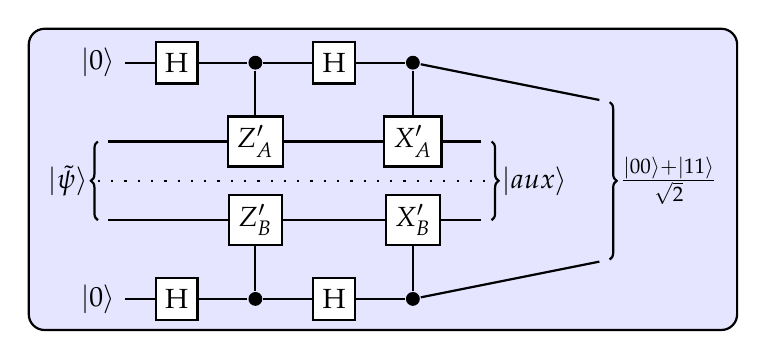
\begin{tikzpicture}[thick]
        %
        % `operator' will only be used by Hadamard (H) gates here.
        % `phase' is used for controlled phase gates (dots).
        % `surround' is used for the background box.
        \tikzstyle{operator} = [draw,fill=white,minimum size=1.5em] 
        \tikzstyle{phase} = [fill,shape=circle,minimum size=5pt,inner sep=0pt]
        \tikzstyle{surround} = [fill=blue!10,thick,draw=black,rounded corners=2mm]
        %
        % Bracket
        \draw[decorate,decoration={brace,mirror},thick] (0,-1) to
    	node[midway,left] (bracket1) {$\ket{\tpsi}$}
    	(0,-2);
        % Qubits
        \node at (0,0) (q1) {$\ket{0}$};
        \node at (0,-1) (q2) {};
        \node at (0,-2) (q3) {};
        \node at (0,-3) (q4) {$\ket{0}$};
        %
        % Column 1
        \node[operator] (op11) at (1,0) {H} edge [-] (q1);
        \node[operator] (op14) at (1,-3) {H} edge [-] (q4);
        %
        % Column 3
        \node[phase] (phase11) at (2,0) {} edge [-] (op11);
	\node[operator] (op22) at (2,-1) {$Z_A'$} edge [-] (q2);
	\node[operator] (op23) at (2, -2) {$Z_B'$} edge[-] (q3);
        \node[phase] (phase14) at (2,-3) {} edge [-] (op14);
        \draw[-] (phase11) -- (op22);
        \draw[-] (phase14) -- (op23);
        %
        % Column 4
        \node[operator] (op31) at (3,0) {H} edge [-] (phase11);
        \node[operator] (op34) at (3,-3) {H} edge [-] (phase14);
        %
        % Column 5
        \node[phase] (phase21) at (4,0) {} edge [-] (op31);
	\node[operator] (op42) at (4,-1) {$X_A'$} edge [-] (op22);
	\node[operator] (op43) at (4, -2) {$X_B'$} edge[-] (op23);
        \node[phase] (phase24) at (4,-3) {} edge [-] (op34);
        \draw[-] (phase21) -- (op42);
        \draw[-] (phase24) -- (op43);
        %
        % Column 6
        \node (end2) at (5,-1) {} edge [-] (op42);
        \node (end3) at (5,-2) {} edge [-] (op43);
        %
        % Bracket
        \draw[decorate,decoration={brace},thick] (5,-1) to
    	node[midway,right] (bracket) {$\ket{aux}$}
    	(5,-2);
        %
        % Column 7
        \node (end1) at (6.5,-0.5) {} edge [-] (phase21);
        \node (end4) at (6.5,-2.5) {} edge [-] (phase24);
        % Dashed line
        \draw[loosely dotted] (0,-1.5) -- (5,-1.5);
        % Bracket
        \draw[decorate,decoration={brace},thick,] (6.5,-0.5) to
    	node[midway,right] (bracket2) {$\frac{\ket{00}+\ket{11}}{\sqrt{2}}$}
    	(6.5,-2.5);
        %
        % Background Box
        \begin{pgfonlayer}{background} 
        \node[surround] (background) [fit = (q1) (op14) (bracket1)(bracket2)] {};
        \end{pgfonlayer}
        %
        \end{tikzpicture}
	\caption{The isometries $\Phi_A$ and $\Phi_B$.}
\end{figure}
To bound $e_{xy} := \norm{ (\Phi_A\x\Phi_B) (\tA_x \x \tB_y) \ket{\tpsi} - \ket{junk} \x (A_x\x B_y) \ket{\EPR{2}}}$,
there are some intermediate steps. Since the derivations are the same as in Ref.~\cite{bamps2015}, 
we only record the key relations here.
\begin{align*}
	&\norm{(Z_B' - Z_B) \ket{\tpsi}} \leq \frac{\sqrt{s}}{c} \sqrt{\epsilon},\\
	&\norm{(Z_B' - Z_A') \ket{\tpsi}} \leq 2 \frac{\sqrt{s}}{c}\sqrt{\epsilon}, \\
	&\norm{(X_B' - X_B) \ket{\tpsi}} \leq \frac{c+1}{s^{3/2}} \sqrt{\epsilon} := \delta_1 \sqrt{\epsilon},\\
	&\norm{(X_B'Z_B'+ Z_B'X_B')\ket{\tpsi}} \leq [\frac{2\sqrt{s}}{c} + \frac{2}{\sqrt{s}} + 2\delta_1 + 
	(\sqrt{2}+\frac{1}{c})(2\frac{\sqrt{s}}{c}+\frac{1+c+s}{c\sqrt{s}})]\sqrt{\epsilon}
	:= \delta_2 \sqrt{\epsilon}.
\end{align*}
Then we can calculate that 
\begin{align*}
	&e_{00} = e_{10} = 2\delta_2 \sqrt{\epsilon}\\
	&e_{20} = 2(\frac{1+c+s}{c\sqrt{s}} + \delta_2) \sqrt{\epsilon}\\
	&e_{01} = e_{02} = e_{11} = e_{12} = [\sqrt{s}+s(2\frac{1+c+s}{c\sqrt{s}} + \delta_1) + 2\delta_2]\sqrt{\epsilon}\\
	&e_{21} = e_{22} = [2\frac{1+c+s}{c\sqrt{s}} + \sqrt{s}+s(2\frac{1+c+s}{c\sqrt{s}} + \delta_1) + 2\delta_2]\sqrt{\epsilon},
\end{align*}
so an upper bound of the error is that
\begin{align}
	\forall x,y \in \{0,1,2\}, e_{xy} \in O((\frac{1}{c^2s^{1/2}} + \frac{1}{s^{3/2}})\sqrt{\epsilon}).
\end{align}
\end{proof}
%%=====================================
\section{The proof of \cref{lm:uo_independ}}
\label{sec:u_and_o}
%%=====================================

We are going to prove 
the set $\{U^k O^l\}$ for $k=0,1\dots d-2$ and $l = 1,2\dots d-1$ forms a basis of the ring of $(d-1)\times (d-1)$ matrices over $\C$
Note that the unitaries $U$ and $O$ defined in the lemma above satisfy the condition $UOU^\dagger = O^r$.
In this proof, we denote the set $\{0,1,2\dots d-2\}$ by $[d-1]$ and the set $\{1,2 \dots d-1\}$ by $[d-1]+1$.
\begin{proof}
We are going to show the $(d-1)^2$ matrices from the set $\{U^k O^l\}_{k \in[d-1], l \in [d-1]+1}$ are linearly independent.
Suppose there exists a set of complex numbers $\{ x_{k,l} \}_{k \in[d-1], l \in [d-1]+1}$
such that 
\begin{align}
	M = \sum_{k=0}^{d-2} \sum_{l=1}^{d-1} x_{k,l} U^k O^l = 0. 
\end{align}
We \hf{define} a set of integers $\{ k_i \}_{i=1}^{d-1}$ such that $r^{k_i} \equiv i \pmod{d}$.
\carl{We shouldn't be making extra assumptions that are not stated in the lemma.  This looks to me more like
a definition of the variables $\{ k_i \}$, rather than an assumption.}
The fact that $r$ is a primitive root of $d$ guarantees that $k_i$'s are distinct.
Then we can group $\{x_{k,l}\}$ into vectors: $\ket{x_{k_1}}, \ket{x_{k_2}} \dots \ket{x_{k_{d-1}}}$,
where $\ket{x_{k_i}}= (x_{k_i, 1}, x_{k_i, 2} \dots x_{k_i, d-1})^\intercal$.
Our goal is equivalent to proving that $\ket{x_{k_i}} = 0$ for all $i$.

We start with proving that $\ket{x_{k_1}} = 0$.
Proving $\ket{x_{k_i}} = 0$ for other $i$ follows a similar argument, so we briefly
discuss about it in the end.
The entry $\bra{1}M\ket{1}$ can be expressed as  
\begin{align}
	\bra{1}M\ket{1} = \sum_{k=0}^{d-2}\sum_{l = 1}^{d-1}\sum_{i=1}^{d-1} x_{k, l}\omega_d^{il}\braket{1}{i (r^{-1})^k}\braket{i}{1}.
\end{align}
For the term $\braket{1}{i (r^{-1})^k}\braket{i}{1} \neq 0$ we must have $i = 1$ and $r^k \equiv 1 \pmod{d}$, or equivalently,
$k = k_1$. We can conclude that 
\begin{align}
	\bra{1}M\ket{1} = \sum_{l = 1}^{d-1} x_{k_1,l}\omega_d^l = 0. 
\end{align}
Similarly we can determine that for all $j = 1,2\dots d-1$,
\begin{align}
	\bra{j}M\ket{j} 
	=  \sum_{k=0}^{d-2}\sum_{l = 1}^{d-1}\sum_{i=1}^{d-1} x_{k, l}\omega_d^{il}\braket{j}{i (r^{-1})^k}\braket{i}{j} 
	= \sum_{l = 1}^{d-1}x_{k_1,l}\omega_d^{jl} = 0.
\end{align}
Hence we get $d-1$ equations with $d-1$ variables, and the linear system is
\begin{align}
	W \ket{x_{k_1}} = 0,
\end{align}
where $W(m,n) = \omega_d^{mn}$. Then we define
\begin{align}
	\tW = 
	\begin{pmatrix}
	1 & 1 \\
	1 & W
	\end{pmatrix}.
\end{align}
First observe that $\tW$ is a Vandermonde matrix, hence it is non-singular.
Next, we define $\ket{\tx_{k_1}} = (0, x_{k_1,1}, \dots x_{k_1,d-1})^\intercal$ 
and prove that it satisfies the condition
that 
\begin{align}
	\tW \ket{\tx_{k_1}} = 0,
\end{align}
which involves $d$ equations. The last $d-1$ equations are given by the assumption and $M$.
We only need to prove that $\sum_{l=1}^d x_{k_1, l} = 0$, which is required by the first row of $\tW$.
It can be proved by summing the known $d-1$ equations as follows
\begin{align}
	0=\sum_{j = 1}^{d-1} \bra{j}M\ket{j}  
	=  \sum_{j=1}^{d-1}\sum_{l = 1}^{d-1}x_{k_1,l}\omega_d^{jl}
	=\sum_{l = 1}^{d-1}x_{k_1,l} (\sum_{j=1}^{d-1} \omega_d^{jl})
	= \sum_{l = 1}^{d-1}- x_{k_1,l}
\end{align}
where we have used the fact that $\sum_{j=1}^{d-1} \omega_d^{jl} =-1$ for all $l = 1,2\dots d-1$.
Since $\tW$ is non-singluar, we know $\ket{\tx_{k_1}} = 0$ which implies that $\ket{x_{k_1}} = 0$.

For $\ket{x_{k_a}}$, we look at entries $\{\bra{j}M\ket{aj}\}_{j=1}^{d-1}$ for $a = 2 \dots d-1$ and get equations
of the form
\begin{align}
	0 = \bra{j}M\ket{aj} = \sum_{l=1}^{d-1} x_{k_a, l} \omega_d^{ajl} 
\end{align}
The corresponding coefficient matrix has value $\omega_d^{amn}$ at coordinate $(m,n)$,
so it is also a submatrix of a Vandermonde matrix. Similar argument gives us that $\ket{x_{k_a}} = 0$.

To summarize, we have proven that $x_{k,l} = 0$ for all $k$ and $l$, which implies that the elements of the set
$\{ U^k X^l \}$ are linearly independent and forms a basis for the ring of all the $(d-1)\times(d-1)$ matrices over $\C$.
\carl{Nice proof.  I like the use of the Vandermonde matrix.  We can think a little about possible simplifications.}
\end{proof}


\end{document}
